\usepackage{ae}
\renewcommand{\ttdefault}{aett}
\usepackage[english]{babel}
\usepackage[latin1]{inputenc}
\usepackage[T1]{fontenc}
\usepackage{epsfig}
\usepackage[Lenny]{fncychap}
\usepackage{setspace}
\usepackage{multicol}
\usepackage{rotating} % Rotating tables sideways
\usepackage{paralist} % For nice Paper I, II etc.
\usepackage{bibentry, natbib}
\usepackage{pseudocode} % Used in LOPI (so far)
\usepackage{supertabular} % Used in the survey
\usepackage{placeins} % \FloatBarrier
\usepackage{url}
\usepackage{ethiop}

\makeatletter
\renewcommand\maketitle{%
  \null
  \thispagestyle{empty}%
  \newlength\tmpoddsidemargin
  \newlength\tmpevensidemargin
  \setlength\tmpoddsidemargin{\oddsidemargin}
  \setlength\tmpevensidemargin{\evensidemargin}
  \setlength\oddsidemargin{0in}
  \setlength\evensidemargin{0in}
  \begin{flushright}
    {\Large \textbf{\@title}\par}

    {\large \textbf{\@author}\par}
  \end{flushright}
  \vspace*{\stretch{1}}
  \begin{center}
%    \includegraphics[height=10cm]{figures/cow}
  \end{center}
  \newpage
  \thispagestyle{empty}%
  \vspace*{\stretch{2}}
  \begin{flushleft}
%    Jacket photo: \@illustration

    \copyright~\@date~\@author \\
    \@institution \\
    Publisher: Blekinge Institute of Technology \\
    Printed by Printfabriken, Karlskrona, Sweden \@date \\
    ISBN \@isbn
  \end{flushleft}
  \newpage
  \thispagestyle{empty}%
  \begin{center}\leavevmode
    Blekinge Institute of Technology \\
    Doctoral Dissertation Series No. {\@series} \\
    ISSN {\@issn} \\
    ISBN {\@isbn} \\

    \vspace*{\stretch{1}} % 1/3 down
    \normalfont
    {\LARGE \textbf{\@title}\par}%

    \vspace*{0.25cm}
    {\Large \@author\par}%

    \vspace*{\stretch{2}} % 2/3 down
    \includegraphics[width=3cm]{/home/ska/figures/BTH_logo_bw}

    \@institution \\
    Blekinge Institute of Technology \\
    Sweden
  \end{center}
  \newpage
  \thispagestyle{empty}%
  \vspace*{\stretch{2}}
  \begin{flushleft}
    \textbf{Contact information}:

    \@author \\
    \@institution \\
    \@location

    email: \texttt{\@email}
  \end{flushleft}
  \null
  \cleardoublepage
  \setlength\oddsidemargin{\tmpoddsidemargin}
  \setlength\evensidemargin{\tmpevensidemargin}
}
\def\series#1{\def\@series{#1}}
\def\isbn#1{\def\@isbn{#1}}
\def\issn#1{\def\@issn{#1}}
\def\institution#1{\def\@institution{#1}}
\def\location#1{\def\@location{#1}}
\def\email#1{\def\@email{#1}}
\def\illustration#1{\def\@illustration{#1}}
\makeatother


\newcommand{\papertitle}[3]{%
  \begin{hyphenrules}{nohyphenation}
    \begin{spacing}{1.0}
      \begin{Large}
        #1
      \end{Large}
      \begin{flushleft}
        \textbf{#2}

        #3
      \end{flushleft}
    \end{spacing}
  \end{hyphenrules}
}

\widowpenalty=50000
\clubpenalty=50000
\parskip 2ex
\bibliographystyle{abbrv}

\begin{document}
\selectlanguage{english}
\nobibliography*
\hyphenation{}

\title{Tools, techniques, and trade-offs when porting large software systems
  to new environments}

\author{Simon K�gstr�m}
\series{2008:07}
\issn{1653-2090}
\isbn{78-91-7295-137-2}
\institution{
  Department of Systems and Software Engineering \\
  School of Engineering}
\location{
  Blekinge Institute of Technology \\
  P.O. Box 520 \\
  372 25 Ronneby \\
  Sweden
}
\email{simon.kagstrom@bth.se}
\illustration{\copyright~2008 XXX}
\date{2008}

\pagestyle{empty} % No page numbers on the first pages
\maketitle

\pagestyle{plain}
\frontmatter
\chapter{Abstract}
% Intro

Computer hardware and software evolve very fast. With the advent of
chip-multi\-processors and symmetric multithreading, multiprocessor hardware
configurations are becoming prevalent. For software, new hardware and
requirements such as security, performance and maintainability drive the
development of new runtime environments, virtual machines and programming
methodologies. These trends present problems when porting legacy
software. Multiprocessor hardware require ports of uniprocessor operating
system kernels while new software environments might require that programs
have to be ported to different languages.

This thesis examines the tradeoff between performance and development effort
for software porting with case studies in operating system porting to
multiprocessors and tool support for porting C and C++ applications to Java
virtual machines. The thesis consists of seven papers. The first paper is a
survey of existing multiprocessor development approaches and focuses on the
tradeoff between performance and implementation effort. The second and third
papers describe the evolution a traditional lock-based multiprocessor port,
going from a serialized ``giant locked'' port and evolving into a
coarse-grained implementation. The fourth paper instead presents an
alternative porting approach which aims to minimize development effort. The
fifth paper describes a tool for efficient instrumentation of programs, which
can be used during the development of large software systems such as operating
system kernels. The sixth and seventh papers finally describe a binary
translator which translates MIPS binaries into Java bytecode to allow
low-effort porting of C and C++ applications to Java virtual machines.


% Contributions

The first main contributions of this thesis is an in-depth investigation of
the techniques used when porting operating system kernels to multiprocessors,
focusing on development effort and performance. The traditional approach used
in the second and third papers required longer development time than expected,
and the alternative approach in the fourth paper can therefore be preferable
in some cases. The second main contribution is the development of a binary
translator that targets portability of C and C++ applications to J2ME
devices. The last two papers show that the approach is functional and has good
enough performance to be feasible in real-life situations.

% Conclusions



\chapter{Acknowledgements}
I would first like to thank my supervisors, \emph{Professor Lars Lundberg} and
\emph{Professor H�kan Grahn} for their help and guidance in my PhD.  studies.
Without their help this thesis would never have got this far.

I am also indebted to the people at Ericsson in �lvsj� and Budapest, primarily
\emph{Hans Nordeb�ck}, \emph{Lars Hennert}, \emph{Stefan Wikstr�m},
\emph{Chengwei Ding} and \emph{Bal�z Tuska} for giving me the opportunity to
work in a real-world industrial project and providing help all the times I got
stuck when working in the project. All my \emph{colleagues}, especially in the
\emph{PAARTS} group and the \emph{BESQ} project have been very helpful during
my work, both as friends and discussion partners. I'd like to extend special
thanks to \emph{Dr. G�ran Fries}, from whom I learned most of what I know
about the MIPS architecture.

Finally, I would like to thank \emph{Linda Ramstedt} for being my loved one
and supporting me throughout the work on this thesis.

This work has been partially funded by Ericsson in �lvsj� together with The
Knowledge Foundation in Sweden under a research grant for the project
``Blekinge -- Engineering Software Qualities
(BESQ)''~(\url{http://www.ipd.bth.se/besq}).


\newcounter{nr:smp-survey}
\newcounter{nr:tsp-giant-lock}
\newcounter{nr:tsp-coarse}
\newcounter{nr:linux-appkern}
\newcounter{nr:lopi}
\newcounter{nr:cibyl}
\newcounter{nr:cibyl-performance}
\newcounter{nr:ska2004}
\newcounter{nr:kagstrom05experiences}

% Paper numbers
\setcounter{nr:smp-survey}{1}
\setcounter{nr:tsp-giant-lock}{2}
\setcounter{nr:tsp-coarse}{3}
\setcounter{nr:linux-appkern}{4}
\setcounter{nr:lopi}{5}
\setcounter{nr:cibyl}{6}
\setcounter{nr:cibyl-performance}{7}
\setcounter{nr:ska2004}{8}
\setcounter{nr:kagstrom05experiences}{9}

\chapter{List of Papers}
\label{sec:intro:publications}
The following papers are included in the thesis

\begin{compactenum}[{Paper} I:]
\item \bibentry{kagstrom05survey}
\item \bibentry{kagstrom05tsp}
\item \bibentry{kagstrom08dicos}
\item \bibentry{kagstrom05appkern}
\item \bibentry{ska05lopi}
\item \bibentry{kagstrom07cibyl}
\item \bibentry{kagstrom08performance}
\end{compactenum}

\begin{flushleft}
  The following papers are related but not included in the thesis.
\end{flushleft}

\begin{compactenum}[{Paper} I:]
\setcounter{enumi}{7}
\item \bibentry{ska2004}
\item \bibentry{kagstrom05experiences}
\end{compactenum}

\begin{flushleft}
  Paper~\Roman{nr:ska2004} is an earlier version of
  Paper~\Roman{nr:linux-appkern} and Paper~\Roman{nr:kagstrom05experiences} is
  an earlier version of Paper~\Roman{nr:tsp-giant-lock}.
\end{flushleft}


\tableofcontents
\listoffigures
\listoftables

\mainmatter
\pagestyle{plain}
\chapter{Introduction}
% TODO
% General introduction
% - Some more work

% MOSTLY DONE?
% Less on MIPS translation
% McCabe is not a devel. effort metric
% Conclusions

% DONE
% Figures in paper III
% Link to cibyl
% Author / Title / published at to each paper
% RQ -> Research question, PQ -> ...
% SPEC -> The standard SPEC bmark
% Moved descr before RQs
% Fixup and read the copy-stuff from lic
% RQ about LOPI
% Contributions of each paper (copy from lic, add)

\section{Background}
The evolution of computer hardware and software moves very fast. In the
hardware domain, storage capacity and processing performance increase at a
high rate. For software, both the hardware evolution and requirements such as
security, performance and maintainability drive the development of new languages,
runtime environments, virtual machines and programming methodologies.

Both hardware and software trends present problems when porting legacy
software. On the hardware side, new hardware generations often require
software porting to benefit from the improved hardware support, and this can
often lead to significant refactoring of the existing code. In the software
domain, new languages or devices locked to specific virtual machines present
difficult problems for maintaining legacy software. In the worst case,
software evolution could require porting to a different language.

This thesis is centered around issues in maintaining legacy software through
hardware changes and new software environments. Special focus has been placed
on case studies in porting of operating system kernels to multiprocessors,
where both traditional lock-based ports and alternative organizations have
been explored, and tool support for porting C and C++ software to Java virtual
machines.

%\textbf{figure placing the papers in this thesis}

%The rest of the introduction is structured as follows.
%Section~\ref{sec:intro:mp} introduces the first topic, multiprocessor
%operating system porting. Section~\ref{sec:intro:language_porting} then gives
%an introduction to the second main topic of language porting.
%Section~\ref{sec:intro:research_questions} presents the research questions in
%the thesis and Section~\ref{sec:intro:research_methodology} talks about the
%research methodology used. Section~\ref{sec:intro:contributions} then gives
%the major contributions in this thesis, and Section~\ref{sec:intro:validity}
%discusses the validity of the results. Related work is presented in
%Section~\ref{sec:intro:related_work} and conclusions can be found in
%Section~\ref{sec:intro:conclusions}.

\section{Multiprocessor porting}
\label{sec:intro:mp}
The first main topic of this thesis is porting uniprocessor operating system
kernels to multiprocessor architectures, discussed in
Paper~\Roman{nr:smp-survey}-Paper~\Roman{nr:linux-appkern}. The main
motivation for multiprocessor operating system porting is the current trend of
moving to multithreaded and multicore processors, which necessitates a
parallelized operating system to make use of the additional processing
resources. The increased use of multithreaded and multicore processors are in
turn motivated by physical constraints, mainly power usage and heat
generation, making scaling with traditional means such as increased clock
frequency difficult~\cite{mudge01power}.
% FIXME: Add asymmetric

The trend of parallelized processors has two main tracks. First, symmetric
multithreading (SMT)~\cite{eggers97simultaneous} is an approach where
processor resources are shared between two or more concurrently running
program threads to allow more efficient use of processor resources. Symmetric
multithreading has been implemented in, e.g., Intel Pentium 4 and Xeon
processors~\cite{marr02hyperthreading} (branded as HyperThreading), and the
2-way multithreaded Sony/IBM Cell processor~\cite{pham05cell}.

The second track is chip multiprocessors (CMPs)~\cite{hammond97singlechip}.
This approach partitions the chip area into two or more mostly independent
processor cores. This means that in the CMP case, the processor resources are
statically allocated to a core whereas the resources in an SMT are dynamically
allocated to a processor thread. The argument for chip multiprocessors is
similar to that for simultaneous multithreading: using many simple cores
provides better energy efficiency and higher operating frequency than using
one complex core.  Chip multiprocessors have been released by
Intel~\cite{intel05multicore} and AMD~\cite{amd05multicore}, and the IBM
POWER4 architecture was released as a dual-core chip in
2001~\cite{kahle99power4}.

Future microprocessors will in many cases contain elements of both the SMT and
CMP approaches. For example, the IBM POWER5~\cite{kalla04power5} and the Sun
Niagara and Niagara 2~\cite{kongetira05niagara, johnson07niagara2}
architectures employ a combination of CMP and SMT technologies. Further, Intel
chip multiprocessors (e.g., Intel Pentium processor Extreme Edition) also
supports HyperThreading. As a result of these trends, a lot of future
microprocessors will be small multiprocessors, and multiprocessors will thus
be used in a large number of systems (also embedded) where uniprocessors were
earlier prevalent.


% Types of oses (more in papir 1): kernel seraialized, parallelized,
% assymetric

Developing programs for multiprocessors presents special problems. While
program threading is possible on uniprocessor computers, truly concurrent
program threads are only available on a multiprocessor. True concurrency can
expose problems which never occurs on a uniprocessor, e.g., concurrent update
of a shared variable. It also makes debugging more difficult since controlling
other threads of execution is harder than on a uniprocessor and presents
timing issues. Simulation can help alleviate some of these problems, but gives
a slow-down and can also be difficult to use if there is specialized hardware
present.

Operating systems need to be adapted to work with the new multiprocessors. It
is not possible to simply allow several processors to start executing in a
uniprocessor operating system, since this would cause unpredictable behavior
when processors concurrently modifies a data structure. Instead, mutual
exclusion is needed in multiprocessor operating systems, e.g., through locking,
so that a processor is stalled or redirected when trying to access a resource
held by another processor.  For good performance, it is important that the
mutual exclusion is fine-grained enough to avoid spending time waiting for
other processors.

However, making modifications to large software bodies such as operating
system kernels is generally very hard.  For instance, Freeman L. Rawson III
writes about this problem when developing the IBM Workplace
OS~\cite{rawson97experience}, which was canceled after six years of
development by a large team of engineers because of engineering problems and
performance issues. In addition, operating system kernels are in many cases
harder to develop and debug than other software systems because of
non-predictability, limited library support, real-time issues, and hardware
effects.

There are performance issues associated with applications running in
multiprocessor operating systems. First, a non-threaded application will not
benefit from a multiprocessor. Second, applications can be categorized into
two broad classes, \emph{compute bound} and \emph{system bound}, where compute
bound applications spend most of their time executing application code and
system bound applications spend a large proportion of their time in-kernel.
Compute-bound applications are not dependent on the parallelization of the
operating system kernel (since these spend little time in-kernel) and can
therefore easier benefit from multiprocessors even on modestly parallelized
operating systems. Third, there are theoretical limits to the performance
obtainable from a multiprocessor. Amdahl's law~\cite{amdahl67validity} states
that since all programs need to execute parts serialized (system calls,
printouts, etc.), the highest speedup attainable with a given number of
processors is:

\begin{displaymath}
  speedup = \frac{1}{t_{serial} + \frac{t_{parallel}}{\#processors}}
\end{displaymath}

With Amdahl's law, the maximum speedup theoretically possible is given by
setting the number of processors to $\infty$. For example, with an application that
spends 10\% of the time running serialized code, the maximum speedup is
$\frac{1}{0.1 + \frac{0.9}{\infty}} = 10$, i.e., even a system with
thousands of processors could never achieve more than a speedup of 10 compared
to a uniprocessor. Amdahl's law also places constraints on processor design as
even with a large number of cores, the performance of serialized execution is
important for the overall speedup~\cite{emer07single}.


Porting an operating system to a multiprocessor computer with good performance
characteristics can therefore demand a tremendous effort, which can pose
problems even to large organizations and experienced software developers. In
this thesis, the tradeoff between performance and implementation effort for
operating system kernels is therefore explored, focusing on techniques for
reducing the development effort.

\FloatBarrier

\section{Language Porting}
\label{sec:intro:language_porting}
The second main topic of this thesis is porting between languages, discussed
in Paper~\Roman{nr:cibyl} and \Roman{nr:cibyl-performance}. There are several
reasons for porting programs to a different language. In some cases,
language-level security can be the main motivation, in other, the platform
might only support a specific language. This type of porting can be very
difficult and time consuming depending on the languages involved, and because
of this, it is an area where tool support can reduce development effort.

% Goal: To maintain in new language, or to just run

Of particular interest is porting of C and C++ programs to Java virtual
machines. This category is important because of the very large body of
programs and libraries written in C and C++, and the prevalence of Java
virtual machines on platforms such as mobile phones. It can also be used to
export C libraries to Java on host machines, which enables distribution of
pure Java archives without the need to resort to calling native code. While
the languages share much of the syntax, there are major differences between
C/C++ and Java:

\begin{itemize}
\item Java enforces type-safety strictly, while it is easy to circumvent in
  C/C++. Many C and C++ programs are also written with implicit dependencies
  on allowing exceptions to type-safety.
\item C/C++ allows pointers to arbitrary memory (even invalid), whereas Java
  uses type-safe references
\item Standard library support is also quite different, for example in how
  file handling is implemented
% More: (Memory image)
\end{itemize}

These things contribute to making this porting difficult and adds to the
advantage of using tool support.

\subsection{Comparison of porting tools}
There are a number of different categories of tools that can be used when
porting between languages:

\begin{itemize}
\item Source-to-source translators, which translate the source code of the
  source language to source code of the destination
  language~\cite{martin02ephedra, jazillan}.
\item Machine emulation that provides an isolated runtime environment for an
  unchanged program.
\item A compiler backend to generate binaries for the target
  language~\cite{axiomsol, cifuentes00UAB}.
\item Binary translation that translates the source binary to binary code for
  the target language (runtime), either online during runtime or offline
  beforehand~\cite{hookway97fx32, bellard05qemu, alliet04nestedvm}.
\end{itemize}

Source-to-source translation can be beneficial when the goal is to switch
language and maintain the code in the new language afterwards. However, in the
case of C/C++, certain parts are inherently difficult to translate. For
example, since pointers in C/C++ can point to any part of memory, it's
difficult to translate these into Java bytecode in a meaningful way.
Source-to-source translation is therefore less useful when the goal is to run
the current software or to keep maintenance of the original source code.
% Examples

Emulation provides a way of keeping the original binary unchanged, but can
require a large runtime environment and also limited performance. For
resource-constrained embedded systems, the size of the runtime environment can
be a major problem. Also, emulating every single instruction can in many
cases make the program too slow for practical use.

Writing a custom compiler backend for the target language / machine has the
best performance potential, but can also be quite complex to implement. The
target machine might also not always be a good match for the compiler. For
example, since Java bytecode is typesafe, it is not possible to access memory
through arbitrary types, which the compiler intermediate format might assume.

Binary translation allows a binary for one architecture to be executed on
another architecture, but without emulating every single instruction such as
in the emulator case. Depending on how it's implemented and the architectures
affected, binary translation can also be fairly efficient.
Paper~\Roman{nr:cibyl} and Paper~\Roman{nr:cibyl-performance} describes
Cibyl, which is a binary translator used for porting C/C++ programs to J2ME
devices, and the rest of this section will focus on binary translation.

\subsection{Binary translation}
Binary translators can be further split in two main types: \emph{dynamic}
binary translators, which perform the translation during runtime, and
\emph{static} binary translators, which perform the translation beforehand. It
is not possible to translate all binaries with static translation because of
e.g., self-modifying code and unclear separation between code and data, but
dynamic translation overcomes these problems. With binaries specifically
targeted for translation, the limitation of static translation can be
overcome.

For the rest of the section, the focus will be on translating 32-bit MIPS
binaries into Java bytecode. MIPS has been selected since it provides a set of
advantages when translating to Java bytecode, which is further described below
and in Paper~\Roman{nr:cibyl}. At first it might seem that the MIPS and Java
bytecode architectures would be very different. MIPS is a traditional
load/store register-based RISC architecture where arithmetic instructions
always operate on 32-bit registers (two sources and one destination) and where
only special load and store instructions can read and write to memory.
Figure~\ref{fig:intro:mips} shows a section of annotated MIPS assembly.

\begin{figure}[htb]
  \centering
  \footnotesize
\begin{verbatim}
1:    lw      v0,16(a0)   # Load 32-bits from mem[a0 + 16] into register v0
      ...
      slt     v0,a1,t1    # v0 = a1 < t1
      bnez    v0, 1b      # if v0 != 0 then goto 1
      sll     v1,a1,0x2   # v1 = a1 << 2
      li      a1,-1       # a1 = -1
      jr      ra          # Jump to address in ra
      move    v0,a1       # v0 = a1, delayed instruction, executed
                          # in pair with the last instruction
\end{verbatim}
  \caption[Sequence of MIPS instructions]{A sequence of MIPS instructions.
    Text after the '\#' sign denotes comments.}
  \label{fig:intro:mips}
\end{figure}

Java bytecode~\cite{lindholm99jvm} is on the other hand based on a stack
machine where arithmetic operations are performed on elements on an operand
stack and pushed back as results. Apart from the operand stack, Java bytecode
also has local variables, which provides register-like storage for temporary
values (and automatic variables for high-level Java code), and class member
variables and static class variables. Local variables are further used to pass
arguments to functions, and the first local variables - corresponding to the
number of arguments passed - are used as function arguments.
Figure~\ref{fig:intro:jbc} illustrates an annotated sequence of Java bytecode
instructions.

\begin{figure}[htb]
  \centering
  \footnotesize
\begin{verbatim}
      iload 5                       ; push local variable 5 on the stack
      iconst_0                      ; push constant 0 on the operand stack
      getstatic CRunTime/memory [I  ; push reference to the CRunTime.memory
                                    ; int vector on the operand stack
      iload 18                      ; push local variable 18 on the operand stack
      iconst_2                      ; push constant 2 on the operand stack
      iushr                         ; push var 18 >> 2 on the stack (popping
                                    ; two items and pushing the result)
      iload 5                       ; push local variable 5 on the stack
      iastore                       ; CRunTime.memory[var 18 >> 2] = var 5
      if_icmpne L_fwd               ; if var 5 != 0 then goto L_fwd
      ...
L_fwd:
\end{verbatim}
  \caption[Sequence of Java bytecode instructions]{A sequence of Java bytecode
    instructions in Jasmin~\cite{jasmin} syntax. Text after the ';' sign
    denotes comments.}
  \label{fig:intro:jbc}
\end{figure}

Java bytecode is designed with security in mind. The bytecode is strictly
typesafe and there are 8-bit \emph{bytes}, 16-bit \emph{shorts}, 32-bit
\emph{integers}, 64-bit \emph{longs}, 32-bit \emph{floats} and 64-bit
\emph{doubles}, all of which are signed. Arithmetic operations on elements on
the operand stack must be performed on two elements of the same type, and the
operand must otherwise be converted manually with a special instruction (for
example \texttt{i2l} which sign-extends an integer to a long. The type must
always be known, which is also the case for local variables and it is
therefore not allowed to read a local variable before it has been assigned.
For each location in the program, these rules must hold for every possible
path to the location.

The bytecode is itself not trusted and the Java virtual machine will verify it
at startup to see that none of the rules are breached. For the more
constrained J2ME JVMs, the verification is instead done in a
\emph{preverifier} beforehand. The virtual machine will throw an exception if
incorrect bytecode is loaded.

Because of the security features and the stack-oriented operation, Java
bytecode is clearly different from MIPS assembly. Even so, the 32-bit MIPS
architecture provide certain benefits as a base for translating in general and
to Java bytecode in particular:

\begin{itemize}
\item Both architectures are big-endian, which simplifies in-memory data
  layout
\item MIPS instructions generally have no side-effects, i.e., do not affect
  flags registers etc. This simplifies each instruction translation since only
  one register need to be updated with a simple write.
\item There is no use of partial registers (e.g., updating a single byte of a
  four byte register)
\item Unaligned memory access can only be done through special instructions
\end{itemize}

There are also some problems with translation to Java bytecode from MIPS
binaries. The first problem is general when performing static translation to
Java bytecode, code is generated beforehand and self-modifying code or
execution of data as code can therefore not be supported. This is only used in
a very limited set of programs, and typically not a problem for programs
written in high-level languages.

The second and most difficult problem is memory access. Because the binary
translator has no control over pointers, translation effectively mandates that
memory is represented by a vector in Java, either in a two-level scheme as in
NestedVM~\cite{alliet04nestedvm} or through a flat scheme as in Cibyl. Memory
is opaque in MIPS assembly, i.e., any address can be accessed at any size
(byte, short, integer) providing the address is aligned on a natural boundary,
whereas Java bytecode does not allow this because of the type safety. This
problem can be solved in different ways: either memory accesses can always be
done at byte-level, reading multiple bytes and combining them to form the
result, or it can be done at a larger size (e.g., 32-bit words), masking out
parts of the word for byte and short access. Chapter~\ref{cha:cibyl} describes
solutions to these translation problems, while
Chapter~\ref{cha:cibyl-performance} outlines optimizations to improve the
performance of the translated code.

\section{Research Questions}
\label{sec:intro:research_questions}

\begin{itemize}
\item \textbf{Primary research question}: How can a good tradeoff between
  performance and development effort be found when moving software across
  hardware or language boundaries?
\end{itemize}

All papers in the thesis deal with different aspects of this question.
Papers~\Roman{nr:smp-survey}-\Roman{nr:linux-appkern} are all related to
operating system porting from uniprocessor to multiprocessor architectures.
Papers~\Roman{nr:cibyl} and \Roman{nr:cibyl-performance} directly address the
problem of porting to new language environments, specifically migration of
legacy C/C++ code to Java virtual machines. Paper~\Roman{nr:lopi} investigates
efficient binary instrumentation, a similar technique to the binary
translation in papers~\Roman{nr:cibyl} and \Roman{nr:cibyl-performance}, and
can be used as a debugging tool for development.

\begin{itemize}
\item \textbf{Research question 1, traditional}: What is the cost and
  performance benefit of performing a traditional symmetric lock-based
  multiprocessor port of an operating system kernel?
\end{itemize}
This question is discussed in Paper~\Roman{nr:smp-survey},
Paper~\Roman{nr:tsp-giant-lock} and Paper~\Roman{nr:tsp-coarse}.
Paper~\Roman{nr:smp-survey} contains an overview of different multiprocessor
porting approaches, and Paper~\Roman{nr:tsp-giant-lock} describes the
implementation of a giant locking scheme in an operating system kernel. This
implementation is then further improved in Paper~\Roman{nr:tsp-coarse}. Having
discussed the traditional approaches, the next goal was to explore the
development effort needed to port an operating system. The next question
relates to these alternative organizations:

\begin{itemize}
\item \textbf{Research question 2, alternative multiprocessor organizations}:
  What are the lower limits of development effort when performing a
  multiprocessor port of an operating system kernel?  Can multiprocessor
  support be added to the operating system without modifying the original
  kernel?
\end{itemize}

The second research question is investigated in Paper~\Roman{nr:smp-survey}
and Paper~\Roman{nr:linux-appkern}. Paper~\Roman{nr:smp-survey} discuss
different approaches to multiprocessor operating systems, while
paper~\Roman{nr:linux-appkern} describe the asymmetric application kernel
approach.

\begin{itemize}
\item \textbf{Research question 3, application instrumentation}: How can
  perturbation and runtime overhead caused by binary instrumentation be
  reduced?
\end{itemize}

Paper~\Roman{nr:lopi} focuses on this question. This technique can be used to
support software porting and debugging, and is also technically closely
related to binary translation.

\begin{itemize}
\item \textbf{Research question 4, binary translation}: How can binary
  translation be employed to facilitate porting of C/C++ applications to a
  Java runtime environment?
\end{itemize}

Paper~\Roman{nr:cibyl} and Paper~\Roman{nr:cibyl-performance} discuss
different aspects of this question, focusing on techniques and performance.

\section{Research Methodology}
\label{sec:intro:research_methodology}
In this thesis, there are two basic issues: performance and development
effort.  To address the first issue, a quantitative benchmark-based approach
has been used. In our studies, a combination of application benchmarks and
synthetic benchmarks has been used for the performance evaluations.
Theoretical analysis, which serves to establish performance limits, has also
been employed in some cases.  The benchmarks have been run either in the
Simics full system simulator~\cite{simics} or on real hardware.  When
evaluating development effort, time has been used as the premier attribute,
but there are also measurements of code properties e.g., number of code
lines and McCabe cyclomatic complexity~\cite{fenton98swmetrics}.

\subsection{Performance Evaluation}
Generally, scripted application benchmarks are used to measure the performance
of a real application with specified input and output~\cite[page
27]{hennessy03computer}. Synthetic benchmarks (or micro benchmarks), on the
other hand, measure specific parts of an execution such as the time required
for a system call.

For the evaluations, a combination of the standard benchmarks SPEC
CPU~2000~\cite{spec2000}, SPLASH~2~\cite{cameron95splash}, more specialized
benchmarks such as Postmark~\cite{katcherpostmark}, and custom synthetic
benchmarks has been used. SPEC CPU~2000 contains a set of mainly compute-bound
single-threaded benchmarks which is often used in computer architecture
research, compiler research, and computer systems performance evaluation.
SPLASH~2 is a benchmark suite with parallel scientific applications commonly
used when evaluating multiprocessor performance. As the SPEC applications are
single-threaded, they will generally not benefit from running on a
multiprocessor machine unless run in a multiprogramming setting. Most of the
SPLASH benchmarks, on the other hand, scale well on multiprocessor machines.

The MinneSPEC reduced workloads~\cite{minnespec} has been used to decrease the
simulation time of SPEC CPU 2000. The MinneSPEC workloads are constructed to
have similar characteristics as the full workloads, although recent work have
shown that periodic sampling gives a closer correspondence to the full
workloads~\cite{yi05techniques}.

Since both SPEC and SPLASH are compute-bound, the operating system will have
only minor influence on the performance. In contrast, the
Postmark~\cite{katcherpostmark} benchmark is a mainly system bound benchmark.
Postmark models the behavior of a mail server, focusing on the performance of
many small files.  Since file system operations to a large extent are handled
in-kernel, Postmark will spend a significant time executing kernel code. The
parallelization of the operating system kernel is therefore very important
when running the Postmark benchmark, and only highly parallel operating system
kernels will scale well with this benchmark.

In some cases it has not been possible to use standard benchmarks. For example
we measure the latency of a~``null''~system call in
Chapter~\ref{cha:linux-appkern}, and for this we use a custom synthetic
benchmark measuring that particular operation. Further, in
Chapter~\ref{cha:tsp-giant-lock}, it was not possible to use standard
benchmarks because of the specialized platform, and configuration problems
also prohibited the use of normal applications on the operating system.
Instead, we constructed a custom application with one thread per processor
that makes it possible to measure performance during varying system call load,
showing how the parallelization of the kernel affects performance.

In Chapter~\ref{cha:lopi}, we use application benchmarks to compare different
instrumentation techniques. The application benchmarks measure the aggregate
behavior of the SPEC applications during the entire run. We measure the number
of instructions executed, cache accesses and misses as well as branches and
branch prediction misses. The measurements were performed on real hardware.

Chapter~\ref{cha:cibyl} and Chapter~\ref{cha:cibyl-performance} use multiple
different benchmarks to show different characteristics. The Mediabench
benchmark suite~\cite{lee97mediabench} is used to compare the performance of
Cibyl to execution on the native host machine (i.e., the overhead of
translated C code compared to native C). We also evaluate two custom written
benchmarks, an A* implementation and Game of life, with which we compare
native Java to the Cibyl-translated binary. Finally, a real-world benchmark, a
GPS navigation application, is used to examine the impact of Cibyl
optimizations.

\subsection{Development Effort Measurement}
Development effort has primarily been evaluated through working hours and lead
time. Chapters~\ref{cha:tsp-giant-lock}, \ref{cha:tsp-coarse} and
\ref{cha:linux-appkern} contain this kind of evaluations. The evaluation
reports the number of developers involved, and the time it took to perform the
design and implementation.

To give further indications of development effort and code complexity, McCabe
cyclomatic complexity has been used.  McCabe cyclomatic complexity measures
the possible number of paths through a function, which is a measure of how
complex the function is to understand and analyze. Generally, the fewer paths
through a function, the fewer test cases are needed to test the
function~\cite{fenton98swmetrics}. The McCabe cyclomatic complexity has been
measured with the \texttt{Pmccabe} tool~\cite{pmccabe}.

The number of source code lines can also give an indication of the development
effort. Except where otherwise stated, the \texttt{sloccount}~\cite{sloccount}
tool by David A. Wheeler, which counts comment-free lines of source code in
many languages, has been used.


\section{Contributions of this thesis}
\label{sec:intro:contributions}
In this section, the papers in the thesis are discussed together with the
contributions made in each paper.

\subsection{Chapter~\ref{cha:paper1} (Paper~I)}
% Purpose/description
Chapter~\ref{cha:smp-survey} presents an investigation of scalability and
development effort for operating system kernels. The purpose of this paper is
to explore the tradeoff between these two quality attributes in the context of
operating system kernels, specifically when porting a uniprocessor kernel to
multiprocessor hardware. In this paper, we identify seven technical approaches
for performing a multiprocessor port and discuss these in the context of
performance and development effort. Further, we perform a case study of how
Linux multiprocessor support has evolved in terms of performance and
development effort for four different versions of the Linux kernel.

% Contributions
The main contribution of this paper is the categorization of technical
approaches for operating system kernels and also a discussion of the
scalability and development effort for these. In the paper, we argue that the
technical approach has a significant effect on the development effort, ranging
from approaches with very low effort such as the approach we present in
Paper~\Roman{nr:linux-appkern} to complete reimplementations with very high
implementation complexity. In the same way, the achieved performance will vary
according to the chosen approach, and generally the expected pattern of higher
development effort correlating with higher scalability holds. We base the
results on a substantial literature study and a case study of the Linux
operating system.

% Research question
This paper connects directly to the main research question, regarding the
performance and development effort tradeoff in multiprocessor operating system
ports, with the paper discussing different technical approaches to operating
system porting.  Further, it also relates to research questions 1 and 2,
\emph{traditional} and \emph{alternative multiprocessor organizations}, on a
higher level, since it gives an overview of both traditional and alternative
systems. The paper is also a foundation for papers~II-IV, which discuss these
two more specific research questions.

\subsection{Chapter~\ref{cha:paper2} (Paper~II)}
% Purpose/description
In Chapter~\ref{cha:tsp-giant-lock}, the design and implementation of
multiprocessor support for a large industrial operating system kernel using a
traditional porting approach is presented. The main purpose of this paper is
to discuss the design options and issues faced when doing the initial port of
a full-scale operating system kernel to multiprocessor hardware. The port is
implemented using a ``giant'' lock which serializes kernel execution. In the
paper, we present implementation details, an initial evaluation of the
implementation, and experiences we gained from the implementation.

% Contributions
There are two main contributions in this paper.  First, we illustrate
technical solutions to common problems found in multiprocessor ports.
For example, we use an approach for processor-local data based on virtual
memory mapping which makes it possible to keep most of the uniprocessor code
unchanged. This approach has a few problems related to multithreaded
processes, and the paper presents a solution to these problems with minimal
changes to the original kernel. The second contribution is a discussion of the
experiences we gained from the implementation. Although we chose a simple
approach, the implementation still required around two years, which was more
time than we had expected.  The main reason for this is the large code-base,
which meant that we had to spend a lot of time understanding the structure
and implementation of the system. Further, the system is highly specialized
and employs a complex configuration process which required us to spend time on
getting the environment to work.

% Research question
With this paper, we discuss the \emph{traditional} research question (research
question 1).  The paper provides implementation experiences from a traditional
port, which was harder to implement than we had expected. The paper also
connects to the main research question.

\subsection{Chapter~\ref{cha:paper3} (Paper~III)}
% Purpose/description
The next paper presents an incremental improvement to the results presented in
Paper~\Roman{nr:tsp-giant-lock}. This paper describes further work on the
multiprocessor port where the locking scheme is relaxed to use coarse-grained
subsystem locks together with fine-grained locks for core data structures.
While the work builds on Paper~\Roman{nr:tsp-giant-lock}, it was implemented
with a larger development team.

% Contributions
The main contribution of this paper is a description of the problems faced
when moving from a multiprocessor port with serialized kernel execution to one
where the kernel is parallelized. The paper also details solutions to the
design challenges and illustrates difficulties in porting operating system
kernels to multiprocessor architectures. This implementation required less
time than the giant-locked prototype, which can be attributed to the larger
development team and reuse of the work done on the previous prototype.

% Research question
In this paper, the \emph{traditional} research question (research question 1)
is again illustrated. The main research question also connects to this work.

\subsection{Chapter~\ref{cha:paper4} (Paper~IV)}
% Purpose/description
The traditional approaches we used in Paper~\Roman{nr:tsp-giant-lock} and
Paper~\Roman{nr:tsp-coarse} allowed us to successfully port a large industrial
operating system kernel, but at the cost of long implementation time.
Chapter~\ref{cha:linux-appkern} presents an alternative approach, the
\emph{application kernel approach}. The application kernel approach provides a
way of adding multiprocessor support without changing the original
uniprocessor kernel. The approach achieves this by running two kernels in
parallel, the original uniprocessor kernel on one processor and a custom
kernel on all other processors. The paper describes an implementation of the
application kernel for Linux, which shows that the approach is feasible in a
real-world setting. We need no changes to neither the Linux kernel nor the
applications.

% Contributions (results)
The main contribution from Paper~\Roman{nr:linux-appkern} is that we show that
it is possible and feasible to add multiprocessor support to an operating
system with minimal changes to the original operating system. We also evaluate
the application kernel approach in terms of performance and implementation
complexity, where we show that the application kernel is comparable in
performance to Linux for compute-bound applications. We therefore conclude
that the application kernel approach would be a viable alternative for
multiprocessor ports of complex operating systems focusing on computationally
intensive applications.

% Connect to research question
Paper~\Roman{nr:linux-appkern} discusses the research question about
\emph{alternative organizations}, showing that alternative organizations can
provide significant advantages in terms of implementation effort. It also
connects directly to the main research question, focusing on an approach with
low development effort.

\subsection{Chapter~\ref{cha:paper5} (Paper~V)}
% Purpose/description
Chapter~\ref{cha:paper5} describes the LOPI framework for program
instrumentation. LOPI is a generic framework for low overhead instrumentation
of program binaries.  LOPI allows arbitrary instrumentation to be added to the
program binary, e.g., performance measurements or path profiling. In LOPI, we
provide a number of low-level optimizations to reduce the perturbation caused
by the instrumentation framework. For example, LOPI tries to improve cache
locality by reusing instrumentation code whenever possible. With these
optimizations, LOPI is able to perform significantly better than the
Dyninst~\cite{buck00dyninst} instrumentation package.

% Contributions (results)
The main contribution of Paper~\Roman{nr:lopi} is that we show how a number
of low-level optimizations can be used to improve program instrumentation
perturbation. LOPI also provides the possibility of automatically adding tests
or performance measurements to large software packages without changing the
source code, or even having access to the source code. We believe that
optimizations such as these can improve the accuracy of measurements and
experiments performed using instrumentation.

% Connect to research question
In this paper, we discuss the research question about \emph{application
  instrumentation}, research question 3. This also connects to the main
research question in that support tools are vital components when working on
large software packages such as operating systems.

\subsection{Chapter~\ref{cha:paper6} (Paper~VI)}
% Purpose/description
In Chapter~\ref{cha:cibyl}, the design and implementation of Cibyl, a binary
translator targeting J2ME devices is presented. Cibyl targets the problem of
porting C and C++ applications to J2ME devices, which only support a Java
runtime environment and therefore makes it difficult to port code written in
other languages. Cibyl overcomes this problem by using the standard GCC
compiler to produce MIPS binaries and thereafter translating these into Java
bytecode.

% Contributions
There are two main contributions of Paper~\Roman{nr:cibyl}. First, the paper
shows how binary translation can be used to target the problem of program
portability successfully. Cibyl has been used to port fairly large
applications to J2ME devices with modest performance overhead in a mostly
automated way. Apart from the binary translation, a generated interface to
Java bytecode is used to provide platform support. Second, the paper
illustrates how the MIPS ABI and extensions to the MIPS ISA can be used to
provide more efficient translation.

% Connect to research question
This paper discusses the \emph{binary translation} research question (research
question 4), focusing on the technology and design choices made. The primary
research question also relates to this paper from side of language boundaries.

\subsection{Chapter~\ref{cha:paper7} (Paper~VII)}
% Purpose/description
Chapter~\ref{cha:cibyl-performance} is an extension of the work performed in
Paper~\Roman{nr:cibyl}. This paper discusses optimizations performed in the
Cibyl binary translator and provides a more extensive performance study than
in Paper~\Roman{nr:cibyl}. It also presents a set of new optimizations not
present in Paper~\Roman{nr:cibyl}.

% Contributions
The main contribution of this paper is to illustrate how optimizations can
improve the performance of translated code. Since the high-level code is
already optimized, the focus of Cibyl optimizations is to reduce the overhead
of translation. Constant propagation of register values, function co-location
and a peephole optimizer are used to this effect. The second contribution of
this paper is a performance study where Cibyl is compared to
NestedVM~\cite{alliet04nestedvm} and native Java. Cibyl performance is found
to be close to native Java for the cases we target, and optimizations improve
performance significantly.

% Connect to research question
As Paper~\Roman{nr:cibyl}, this paper discusses the \emph{binary translation}
research question (research question 4) but focusing on the performance side
of it. It also connects to the main research question from the side of
language porting.

\section{Validity of the Results}
\label{sec:intro:validity}
This section presents a number of threats to the validity of the studies. The
discussion is centered around threats to the generalizability (or external
validity) and the internal validity.

\subsection{Generalizability, External Validity}
External validity refers to the possibility of generalizing the study results
in a setting outside of the actual study~\cite[page 106]{robson02realworld}.
There are two threats to the generalizability of the work which are
applicable to all papers in this thesis. One dimension is hardware, i.e., if
the results are generalizable to larger hardware configurations or portable to
entirely different platforms. The other dimension is software, i.e., if the
results are generalizable to other software platforms.

The hardware generalizability is addressed in several ways. First,
Paper~\Roman{nr:lopi} describes low-level optimizations which are closely tied
to the target hardware and therefore hard to port and generalize. In this
case, this is inherent in the approach since the optimizations are
intentionally system dependent. Paper~\Roman{nr:linux-appkern},
Paper~\Roman{nr:tsp-giant-lock}, and Paper~\Roman{nr:tsp-coarse}, describe
multiprocessor ports of two operating system kernels, both targeting Intel
IA-32.  While many low-level aspects of these ports are architecture-specific,
e.g., startup of secondary processors, most of the code (locking, etc.) is
common between architectures which makes most of the results valid for other
architectures as well. The application kernel approach presented in
Paper~\Roman{nr:linux-appkern} poses a set of requirements on the
architecture, e.g., processor-local interrupt handlers. These requirements are
discussed for different architectures, and in most cases these are trivially
fulfilled. It is therefore likely that the application kernel can be easily
ported to a large set of hardware platforms.

Hardware scalability threats has been further addressed by using the Simics
full-system simulator~\cite{simics} to simulate hardware configurations with
between one and eight processors. Simics gives the possibility to test larger
configurations than the available hardware, and is used to examine the
scalability in Paper~\Roman{nr:smp-survey} and Paper~\Roman{nr:linux-appkern}.
Further, Simics has been used in Paper~\Roman{nr:lopi} to study detailed
application behavior, which is hard or impossible using traditional hardware
measurements.

To improve the software generalizability, standard benchmarks such as SPEC CPU
2000, SPLASH 2, and Postmark have been employed in
Paper~\Roman{nr:smp-survey}, Paper~\Roman{nr:linux-appkern} and
Paper~\Roman{nr:lopi}. Using standard benchmarks allow the studies to be
replicated and also to be compared with other similar studies.  It is also
shown that the application kernel approach is fairly independent of the
original uniprocessor kernel, since most of the code from an in-house kernel
implementation could be reused for the Linux port of the application kernel.
This suggests that the application kernel approach should be possible to reuse
mostly unmodified for ports to other operating systems.

The specialized benchmarks used in Paper~\Roman{nr:tsp-giant-lock},
Paper~\Roman{nr:cibyl} and Paper~\Roman{nr:cibyl-performance} are harder to
generalize. Still, since the benchmark in Paper~\Roman{nr:tsp-giant-lock} is
very basic, measuring the parallelization of the operating system kernel, it
is still possible to compare to similar benchmarks on other operating systems.
However, since it was not possible to run full-scale applications, it is
difficult to generalize the performance results to a production environment.

In Paper~\Roman{nr:cibyl-performance}, two specialized benchmarks are used,
one being an implementation of the A* algorithm and the other
FreeMap~\cite{shabtai07roadmap}, a GPS navigation software. The A* algorithm
implementation is used to be able to compare the same software across
different languages (C and Java) since it is implemented in the same way on
both places. The A* implementation also allows comparison between different
data structure layouts. FreeMap is used to provide performance characteristics
of a real-world benchmark. The A* benchmark provides an indication of
performance limits of the Cibyl implementation while the FreeMap benchmark
should be generalizable to the same class of graphical applications.

\subsection{Internal Validity}
Internal validity refers to how well a study can establish the relationship
between cause and effect~\cite[page 103]{robson02realworld}. For example, in a
performance comparison between two versions of a multiprocessor operating
system kernel (which was done for the Linux kernel in
Paper~\Roman{nr:smp-survey}), a finding might be that the later version of the
kernel has better performance.  However, it is not possible to draw the
conclusion that this is because of improved multiprocessor support in the
newer version since other factors such as a better file system implementation,
optimized virtual memory handling, etc., also affects performance. In
Paper~\Roman{nr:smp-survey}, the Linux kernel performance results is therefore
normalized against a baseline of uniprocessor performance in the 2.0 kernel.
The benchmark also shows that the performance, even on the uniprocessor, is
around three times higher on 2.6 than on 2.0 for the same benchmark.

One validity concern for the work is the use of a full-system simulator
compared to real hardware. If the simulator is not accurate enough, the
results will diverge from real hardware. There are two aspects of this. First,
the Intel IA-32 instruction set is very complex to simulate accurately,
compared to many RISC architectures. On current processors, IA-32 instructions
are split up in RISC-like micro instructions~\cite{intel02sdm1} before they
are executed, and the actual microcode implementation can vary greatly between
different implementations of the architecture. Although Simics simulates
microcode for the Pentium 4, the available hardware at the time of the
experiments (Pentium~Pro, Pentium~II, and Pentium~III) is quite different from
Pentium 4 and microcode simulation was therefore not employed.

The second aspect is cache simulation. Since main memory is several magnitudes
slower than the processor, caches that store frequently used data are needed
to hide memory latency~\cite{hennessy03computer}. A miss in the cache can
stall the processor for significant durations. For multiprocessors, another
source of latency is traffic to keep the cache contents on different
processors coherent. Simics can simulate the complete memory hierarchy
including caches and coherence traffic. In Paper~\Roman{nr:lopi}, memory hierarchy
simulation has been used to show detailed behavior of the instrumentation of
SPEC applications (Section~\ref{sec:lopi:measurements} in
Paper~\Roman{nr:lopi}), whereas measurements on real hardware were used to
get aggregate values.

In Paper~\Roman{nr:linux-appkern}, the memory hierarchy was not simulated
since the purpose of the simulations have been to show scalability limits.
There are known performance issues with the application kernel prototype
related, e.g., to memory layout, which are not implemented and would give a
disproportionally large disadvantage in the cache simulation.

The benchmarks in Paper~\Roman{nr:cibyl} and \Roman{nr:cibyl-performance}
targeting J2ME devices are performed in an emulated environment, the Sun J2ME
emulator which builds on the Sun K virtual machine~\cite{sun00kvm}. Since the
target domain is mobile phones, there can be some differences compared to
running on actual hardware which may run other JVMs and have different
implementations of support libraries. Where possible, the benchmarks have
therefore been run on a set of different JVMs, which have different
performance characteristics. The general tendency is possible to discern from
these tests, although actual numbers will vary between devices.

Reproducibility, the ability of other researchers to reproduce the results, is
another important aspect. For the papers in this thesis, this has been
adressed in two ways. First, there are detailed descriptions in each paper of
how the experiments have been performed. Second, the source code for the work
in Papers \Roman{nr:linux-appkern}, \Roman{nr:lopi}, \Roman{nr:cibyl} and
\Roman{nr:cibyl-performance} is freely available for download and inspection.

\section{Related work}
\label{sec:intro:related_work}
The related work has been divided after the subsidiary research questions.
Since Paper~\Roman{nr:smp-survey} contains both traditional multiprocessor
ports and alternative organizations, this paper is discussed in the context of
the corresponding subsidiary questions.

% FIXME: Try to find something common for all

\subsection{Traditional Multiprocessor Ports}
The traditional giant locking organization used in
Paper~\Roman{nr:tsp-giant-lock} has been used in a number of other systems.
For example, early versions of Linux and FreeBSD both used a giant locking
approach~\cite{beck98linux, lehey03freebsd}. Similarly, many operating systems
have gone through phases with subsystem locks like in
Paper~\Roman{nr:tsp-coarse}, including Linux. As discussed in
Paper~\Roman{nr:smp-survey}, the giant locking approach is a feasible approach
for initial multiprocessor ports since it is relatively straightforward to
implement and also possible to incrementally enhance by making the locks more
fine-grained.

The system used in Paper~\Roman{nr:tsp-giant-lock} and
Paper~\Roman{nr:tsp-coarse} is a cluster operating system kernel running on
IA-32 hardware, and there exists other similar systems. While generic
operating system kernels such as Linux~\cite{beowulf},
Windows~NT~\cite{microsoft05cluster} and Sun Solaris~\cite{sun99cluster} have
been used to build cluster systems, there are fewer dedicated operating system
kernels for clusters. One example of such a system is
Plurix~\cite{goeckelmann03plurix}. Plurix is a kernel which, like the system
presented in Papers \Roman{nr:tsp-giant-lock} and \Roman{nr:tsp-coarse},
employs distributed objects which are kept coherent through a
transaction-based scheme. However, Plurix only runs on uniprocessor nodes and
is also based on Java, whereas the multiprocessor port in Papers
\Roman{nr:tsp-giant-lock} and \Roman{nr:tsp-coarse} supports both Java and C++
development.

\subsection[Alternative Operating System organizations]{Alternative Multiprocessor Operating System Organizations}
The work in Paper~\Roman{nr:linux-appkern} has several connections to other
work. First, there is other work done related to employing restricted
knowledge in systems. For example, Arpaci-Dusseau et
al.~\cite{arpacidusseau01information} propose a method where
``gray-box''~knowledge about algorithms and the behavior of an operating
system is used to acquire control and information about the system without
explicit interfaces or operating system modification. This idea is similar to
Paper~\Roman{nr:linux-appkern} in that it restricts the information needed
about the kernel to knowledge about the algorithms, but it differs in the
intended purpose: controlling operating system behavior compared to adding
multiprocessor support. Zhang et al.~\cite{zhang03qos}, have done work where
the operating system kernel is modified to provide quality of service
guarantees to large unmodified applications. This work takes the opposite
approach to Paper~\Roman{nr:linux-appkern}: the kernel is explicitly modified
to suit applications while the approach in Paper~\Roman{nr:linux-appkern}
avoids modifying the kernel and actually needs no modifications to the
applications either.

Second, the technical approach described in Paper~\Roman{nr:linux-appkern} is
related to older operating system kernels organized as master-slave systems
and to certain distributed systems. For example, Goble and
Marsh~\cite{goble82dualvax} describe the hardware and software implementation
of a master-slave VAX multiprocessor. Because of the emergence of
heterogeneous multiprocessors, there has been renewed interest in master-slave
systems recently~\cite{seo07masterslave}. Paper~\Roman{nr:linux-appkern} uses
the same structure as master-slave systems in that it restricts kernel
operations to one processor.  However, master-slave systems modify the
original kernel to add the multiprocessor support whereas the application
kernel approach adds the support outside of the original kernel.

The MOSIX distributed system~\cite{mosix}, which provides support for
distributing standard applications transparently on a cluster, also uses an
approach similar to the application kernel. MOSIX redirects kernel operations
to the ``unique home node''~of an application to provide a single-system image
cluster.  The approach in Paper~\Roman{nr:linux-appkern} works the same way,
but on a multiprocessor computer instead of a cluster.

%Cell processor: similar idea to appkernel
%\url{http://www.research.scea.com/research/html/CellGDC05/26.html}

\subsection{Program Instrumentation}
There are several instrumentation tools which share properties with LOPI.
First, there are a number of tools which directly employ binary rewriting
similar to LOPI. For example, Etch~\cite{etch} is a tool for rewriting Windows
binaries on the IA-32 architecture, which like LOPI has to deal with the
complexities of an instruction set with variable-sized instructions.
EEL~\cite{eel} and ATOM~\cite{atom} also rewrite binaries, but have been
constructed for the SPARC and Alpha architectures, respectively, which use
fixed-sized instructions and are therefore better adapted to instrumentation.
Both EEL and ATOM provide frameworks to build tools to instrument programs,
unlike LOPI which only provides basic instrumentation since the purpose of
LOPI is to provide low-level support for building instrumentation tools.

Dyninst~\cite{buck00dyninst}, Valgrind~\cite{valgrind} and Pin~\cite{luk05pin}
use a different approach than LOPI for the instrumentation. These tools allow
programs to be dynamically instrumented, i.e., adding instrumentation to the
program in-memory after the program has been started. Valgrind works by
dynamically translating all instructions of the program, inducing a high
overhead but being general and allowing many program transformation. Although
LOPI only instruments binaries, the optimizations performed by LOPI is
applicable to dynamic instrumentation as well.

% Add simics...

\subsection{Binary translation}
Binary translation, as used in Cibyl, is also closely related to the binary
instrumentation in LOPI. Of other related work,
NestedVM~\cite{alliet04nestedvm} (which has been discussed earlier) is clearly
the most similar to Cibyl, also being a static off-line binary translator
targeting Java bytecode. Valgrind~\cite{valgrind} is a dynamic binary
translator which targets debugging and inspection support, e.g., through a
heap management checker, and uses similar techniques as Cibyl.

A traditional problem in static binary translators is separating code from
data~\cite{altman00welcome}, i.e., detecting if a part of the binary executes
as code or is data. Cibyl does not have this problem by virtue of being a
development environment: Cibyl requires the source code and compiles binaries
with symbol and relocation data retained.

Dynamic binary translators~\cite{hookway97fx32, bala00dynamo, buck00dyninst}
get around the code vs data problem by performing the translation at runtime
and therefore only translates code as it executes. However, since Cibyl is
targeting an embedded system, runtime memory and code size overhead which can
result from doing runtime translation is a problem. Java virtual machines also
do not allow loading dynamically generated code with a smaller than class
granularity~\cite{lindholm99jvmspec}, which would mean a large overhead when
calling generated code.

Another approach to the problem of executing C or C++ applications on a Java
virtual machine is to provide a compiler backend generating Java bytecode.
This has been done in the Axiomatic solutions~\cite{axiomsol} multi-platform C
compiler and as a part of the University of Queensland Binary Translator
project~\cite{cifuentes00UAB}. Both these are based on an old version of GCC,
and both face the problem of keeping the port updated with GCC releases, which
is done automatically with the Cibyl approach (being independent of GCC
version). Cibyl also automatically benefits from GCC optimization improvements
with new versions. The benchmarks also show that the translation of MIPS
binaries can be done with relatively low overhead, reducing the potential
performance advantage of writing a targeted compiler backend.


\section{Conclusions}
\label{sec:intro:conclusions}
The primary goal of this thesis has been to look into the tradeoff between
performance and development effort for porting of software systems to new
environments. I have investigated this tradeoff both for operating system
porting from uniprocessors to multiprocessors and porting of C/C++
applications to Java environments. Operating system porting was studied in
Paper~I-IV and C/C++ porting to JVMs was studied in
Paper~\Roman{nr:cibyl}-\Roman{nr:cibyl-performance}. Paper~\Roman{nr:lopi}
presents a tool for program instrumentation which can be used during the
development of large software systems in general, covering both major topics.

% Answer questions
The primary research question has been discussed in all papers in the thesis.
For multiprocessor operating systems, Paper~\Roman{nr:tsp-giant-lock} and
Paper~\Roman{nr:linux-appkern} present two radically different approaches to
an initial port to a multiprocessor. In Paper~\Roman{nr:tsp-giant-lock}, a
traditional kernel parallelization effort is described, which was found to be
time consuming and difficult to scale. The application kernel approach in
Paper~\Roman{nr:linux-appkern} implements multiprocessor support for Linux
with minimal changes to the uniprocessor kernel. The application kernel
approach also has limited scalability, but requires less knowledge and
modifications of the original kernel. The approach in
Paper~\Roman{nr:tsp-giant-lock} still has advantages, however. First, it
balances processing among all CPUs, which the asymmetric application kernel
approach does not do. Second, it provides a base for further incremental
improvements, which was done in Paper~\Roman{nr:tsp-coarse}. These three
papers illustrate the different tradeoffs between performance and development
effort, ranging from the application kernel approach which focuses on
development effort to the coarse-grained implementation in
Paper~\Roman{nr:tsp-coarse} where a large effort was spent to achieve
scalability.

Papers~\Roman{nr:cibyl} and \Roman{nr:cibyl-performance} focuses on the
language boundary part of the primary research question. The Cibyl approach is
placed between the three extremes of re-implementing the source code in Java,
implementing a full compiler backend to produce Java bytecode (both of which
should give better performance) or providing pure emulation, which requires
less implementation at the cost of lower performance. With the optimizations
made, Cibyl is a viable alternative to the full compiler backend at lower
maintenance cost (automatically benefiting from new GCC releases). Between the
two other main topics, Paper~\Roman{nr:lopi} about the LOPI binary
instrumentation framework deals with tool support to facilitate development,
and also uses similar techniques as Cibyl.

Papers~\Roman{nr:tsp-giant-lock} and \Roman{nr:tsp-coarse} also discuss
research question 1 about the cost of a traditional symmetric lock-based
multiprocessor port. The findings indicate that there is a significant cost
associated with the traditional porting methods. For the first giant-locked
port, a large proportion of the time was spent to grasp the functionality of
the uniprocessor code, which was required to parallelize execution. For the
coarse-grained port, the largest obstacles has instead been the move from
completely serialized kernel execution (as in both the uniprocessor and the
giant locked kernel) to a parallelized kernel. This brings along many ordering
and timing issues which are not otherwise present. The larger team and
experience gained from the prototype in Paper~\Roman{nr:tsp-giant-lock} meant
that this work still required less time than the prototype.

As a contrast to the first research question, research question 2 about
alternative multiprocessor organizations is investigated in
Paper~\Roman{nr:linux-appkern}. In this paper, we show that alternative
asymmetric organizations such as the application kernel approach can provide
shorter porting time at a cost of some overhead for kernel-bound tasks. The
paper also shows that it is feasible to add multiprocessor support to an
operating system kernel without modifications of the uniprocessor kernel.

Research questions 3 and 4 are answered in Papers~\Roman{nr:lopi},
\Roman{nr:cibyl} and \Roman{nr:cibyl-performance}. The LOPI paper shows
techniques which can be employed to reduce perturbations of instrumented
programs and illustrates the importance of architecture-dependent techniques
to reduce perturbation. The two Cibyl papers in turn show that static binary
translation is a feasible approach to provide portability of C and C++
programs to Java virtual machines with adequate performance in real-life
settings and low maintenance cost.

% The minor questions

%%% Local Variables: 
%%% mode: latex
%%% TeX-master: t
%%% End: 



\chapter{Paper~I}
\papertitle{Scalability vs. Development Effort for Multiprocessor Operating System Kernels}
  {Simon K�gstr�m, H�kan Grahn, Lars Lundberg}
  {Submitted for journal publication, March 2008}
\label{cha:paper1}
\label{cha:smp-survey}
% L�gg till: An Effective Design of Master-Slave Operating System Architecture for Multiprocessor Embedded Systems
\section{Introduction}

With the advent of multicore and simultaneous multithreaded processors, shared
memory multiprocessors are becoming very common. This makes operating system
support for multiprocessors increasingly important. Some operating systems
already include support for multiprocessors, but many special-purpose
operating systems still need to be ported to benefit from multiprocessor
computers. To get good multiprocessor support, a number of challenges
involving concurrency issues, have to be solved, and how these are handled
affect the engineering time needed for the multiprocessor implementation.

There are a number of possible technical approaches when porting an operating
system to a multiprocessor, e.g., introducing coarse or fine grained locking
of shared resources in the kernel, introducing a virtualization layer between
the operating system and the hardware, or using the master-slave and other
asymmetric approaches.

The development effort and lead time for porting an operating system to a
multiprocessor vary depending on the technical approach used. The technical
approach also affects multiprocessor performance.  The choice of technical
approach depends on a number of factors; two important factors are the
available resources for doing the port and the performance requirements on the
multiprocessor operating system. Consequently, understanding the performance
and development cost implications of different technical solutions is crucial
when selecting a suitable approach.

In this paper we identify seven technical approaches for doing a
multiprocessor port. We also provide an overview of the development time and
multiprocessor performance implications of each of these approaches.  We base
our results on a substantial literature survey, and also provide a case study
concerning the development effort and multiprocessor performance (in terms of
scalability) of different versions of Linux. We have limited the study to
operating systems for shared memory multiprocessors.

The rest of the paper is structured as follows.
Section~\ref{sec:survey:challenges} describes the challenges faced in a
multiprocessor port. In Section~\ref{sec:survey:categorization} we present a
categorization of porting methods, and
Section~\ref{sec:survey:implementations} then categorizes a number of existing
multiprocessor systems. In Section~\ref{sec:survey:linux}, we describe our
Linux case study, and finally discuss our findings and conclude in
Section~\ref{sec:survey:discussion}.

\section{Multiprocessor Port Challenges}
\label{sec:survey:challenges}
A uniprocessor operating system needs to be changed in a number of ways to
support multiprocessor hardware. Some data structures must be made CPU-local,
like for example the currently executing process. The way CPU-local data
structures are implemented varies. One approach is to replace the affected
variables with vectors that are indexed with the CPU number. Another is to
cluster the CPU-local data structures in a virtual memory region and map this
region to different physical memory pages for each CPU.

In a uniprocessor kernel where processes cannot be preempted in-kernel, the
only source of concurrency issues is interrupts, and disabling interrupts is
then enough for protection against concurrent access. On multiprocessors,
disabling interrupts is not enough as it only affects the local processor.
Also, multiple processors accessing shared memory at the same time can cause
conflicts even outside interrupt context. A locking scheme is therefore
needed. Locking can be implemented in different ways, e.g., through spinlocks
or semaphores. Spinlocks are implemented by letting the processor do a busy
wait for a held lock. Acquiring a semaphore usually involves a context switch
to let other processes execute, and is therefore better suited if the lock is
held for a long time. Kernels which support in-kernel process preemption
(i.e., involuntarily suspending threads within the kernel) need protection of
shared data structures even on uniprocessors.

Locking affect both performance and development time of multiprocessor
operating systems. A held spinlock means that another processor cannot enter a
section of code or access a region of data, which locks the processor out from
useful work. At the same time, race conditions can occur if data is not
properly protected by locks, and careful examination of dependencies between
locks etc. adds to the development time.

Many modern processors employ memory access reordering to improve performance.
Therefore, memory barriers are sometimes needed to prevent inconsistencies.
For example, a structure needs to be written into memory before the structure
is inserted into a list for all processors to see the updated data
structure. Further, debugging, which is hard even in uniprocessor operating
systems, become more difficult when several processors execute in the kernel
at the same time.


\begin{figure*}[t!]
  \begin{tabular}{ccc}
    \epsfig{width=0.30\linewidth, file=figures/smp-survey/giant_lock}\hspace{0.22cm} & \epsfig{width=0.30\linewidth, file=figures/smp-survey/coarse_grained}\hspace{0.22cm} & \epsfig{width=0.30\linewidth, file=figures/smp-survey/fine_grained} \\
    (a) Giant lock & (b) Coarse-grained & (c) Fine-grained \\
    \\
    \epsfig{width=0.30\linewidth, file=figures/smp-survey/master_slave}\hspace{0.22cm} & \epsfig{width=0.30\linewidth, file=figures/smp-survey/appkern}\hspace{0.22cm} & \epsfig{width=0.30\linewidth, file=figures/smp-survey/piglet} \\
    (d) Master-slave & (e) The Application kernel & (f) Piglet \\
  \end{tabular}
  \caption[Multiprocessor operating system oganizations.]{\emph{Continued on
      next page}}
  \label{fig:survey:methods}
\end{figure*}

\begin{figure*}[t]
  \begin{tabular}{ccc}
    \epsfig{width=0.30\linewidth, file=figures/smp-survey/cache_kernel}\hspace{0.22cm} & \epsfig{width=0.30\linewidth, file=figures/smp-survey/virtualization}\hspace{0.22cm} & \epsfig{width=0.30\linewidth, file=figures/smp-survey/k42} \\
    (g) Cache-kernel & (h) Virtualization & (i) K42 \\
  \end{tabular}

  \begin{flushleft}
  Figure~\ref{fig:survey:methods}: Multiprocessor operating system
  organizations. Thick lines show locks and the flash symbol denote system
  calls or device interrupts. The figure shows both categories and examples of
  systems.
  \end{flushleft}
\end{figure*}

\section{Categorization}
\label{sec:survey:categorization}
We have categorized the porting approaches into the following implementation
approaches: \emph{giant locking}, \emph{coarse-grained locking},
\emph{fine-grained locking}, \emph{lock-free}, \emph{asymmetric},
\emph{virtualization}, and \emph{reimplementation}. Other surveys and
books~\cite{mukherjee93survey, schimmel94unix} use other categorizations,
e.g., depending on the structuring approach (microkernels and monolithic
kernels). In this section we describe the properties of each of these
implementation methods.


\subsection{Locking-based schemes}

\subsubsection{Giant Locking}
With giant locking (Figure~\ref{fig:survey:methods}a), a single spin lock
protects the entire kernel from concurrent access. The giant lock serializes
all kernel accesses, so most of the uniprocessor semantics can be kept. Giant
locking requires small changes to the kernel apart from acquiring and
releasing the lock, e.g., processor-local pointers to the currently executing
process.  Performance-wise, scalability is limited by having only one
processor executing in the kernel at a time.

Giant locking presents only a minor risk for deadlocks and race conditions
since the kernel access is serialized. The number of places the giant lock
needs to be taken corresponds to the number of entry points into the kernel,
which greatly simplifies the implementation. In terms of porting, the giant
locking approach provides a straightforward way of adding multiprocessor
support since most of the uniprocessor semantics of the kernel can be kept.
However, the kernel also becomes a serialization point, which makes scaling
very difficult for kernel-bound benchmarks. As a foundation for further
improvements, giant locking still provides a viable first step because of its
relative simplicity.

\subsubsection{Coarse-grained Locking}
Coarse-grained locks protect larger collections of data or code, such as
entire kernel subsystems as shown in Figure~\ref{fig:survey:methods}b.
Compared to giant-locking, coarse-grained locks open up for some parallel work
in the kernel.  For example, a coarse-grained kernel can have separate locks
for the filesystem and network subsystems, allowing two processors to
concurrently execute in different subsystems. However, inter-dependencies
between the subsystems can force an effective serialization similar to giant
locking. If subsystems are reasonably self-contained, coarse-grained locking
is fairly straightforward, otherwise complex dependencies might cause data
races or deadlocks.

\subsubsection{Fine-grained Locking}
Fine-grained locking (Figure~\ref{fig:survey:methods}c), restricts the locking
to individual data structures or even parts of data structures.  Fine-grained
locking allows for increased parallelism at the cost of more lock invocations
and more complex engineering. Even fine-grained implementations will sometimes
use coarse-grained locks, which are more beneficial for uncontended data.

Finer granularity of the locks at makes the implementation more prone to
errors such as race conditions and deadlocks, especially compared to the giant
locking approach.

\subsection{Lock-free Approaches}
Using hardware support, it is possible to construct lock-free operating
systems. Lock-free algorithms rely on instructions for atomically checking and
updating a word in memory (compare-and-swap, CAS), found on many CPU
architectures. However, for efficient implementation of lock-free algorithms,
a CAS instruction capable of updating multiple locations is needed, e.g.,
double CAS (DCAS). Simple structures such as stacks and lists can be
implemented directly with CAS and DCAS, while more complex structures use
versioning and retries to detect and handle concurrent
access.~\cite{massalin92lockfree}

A completely lock-free operating system relies on these specialized data
structures. Lock-free data structures are sometimes hard to get correct and
can be inefficient without proper hardware support~\cite{doherty04dcas}, which
limits the scalability of completely lock-free approaches. Also, transforming
an existing kernel to lock-free operation requires a major refactoring of the
kernel internals, so the development costs of a lock-free kernel is likely to
be high.

\subsection{Asymmetric Approaches}
It is also possible to divide the work asymmetrically among the processors.
Asymmetric operating systems assign processors to special uses, e.g., compute
processors or I/O handling processors. Such a system might be beneficial for
cases where there is a high I/O load, or to simplify operating system ports
(as discussed in Section~\ref{sec:survey:asymmetric}).

Since asymmetric systems can be very diverse, both the implementation cost and
scalability of these systems will vary.

\subsection{Virtualization}
A completely different method is to partition the multiprocessor machine into
a virtual cluster, running many OS instances on shared hardware
(Figure~\ref{fig:survey:methods}h). This category can be further
subdivided into fully virtualized and paravirtualized systems, where the
latter employs operating system modifications and virtual extensions to the
architecture to lower virtualization overhead or handle hardware limitations
which makes full virtualization hard to achieve~\cite{robin00intel}.

The virtualizing layer, called a Hypervisor, runs at a higher privilege level
than the operating system kernel. The Hypervisor performs handling and
multiplexing of virtualized resources, which makes the Hypervisor less
demanding to implement than a full operating system kernel. As virtualization
also allows existing uniprocessor operating systems to run with small or no
modifications, the development costs of a port is limited.

As discussed above, not all processor architectures are well suited for full
virtualization. Recent processors therefore have hardware support for
virtualization~\cite{uhlig05virtualization, amd05pacifica}, e.g., through
providing an extra set of privilege levels and trapping on access to
privileged instructions. With this hardware extensions, unmodified operating
systems can run on top of a Hypervisor, although the performance will be
limited by emulation of hardware devices.


\subsection{Reimplementation}
A final approach is to reimplement the core of the kernel for multiprocessor
support and provide API/ABI compatibility with the original kernel.  While
drastic, this can be an alternative for moving to large-scale multiprocessors,
when legacy code might otherwise limit the scalability.

\section{Operating System Implementations}
\label{sec:survey:implementations}
In this section, we discuss different implementations of multiprocessor ports
representing the different porting approaches presented.
Table~\ref{tab:survey:categorization} provides a summary of the discussed
systems.


\subsection{Giant-locking Implementations}

Many multiprocessor ports of uniprocessor operating systems are first
implemented with a giant locking approach, e.g., Linux 2.0~\cite{beck98linux},
FreeBSD~\cite{lehey03freebsd}, and other kernels~\cite{kagstrom05experiences}.
Later releases relaxes the locking scheme with a more fine-grained approach. We discuss
the Linux giant locking more in detail in Section~\ref{sec:survey:linux}.  The
industrial kernel described in~\cite{kagstrom05experiences} uses a giant
locking approach for the first version of the port. The performance of the
port was found to be limited due to a large proportion of in-kernel time. This
port was shown to be difficult due to a large code size and a single-person
development team.

The QNX Neutrino microkernel~\cite{qnx} also protects the kernel with a giant
lock. Latency for QNX is limited by the small amount of code actually executed
within the kernel. However, as most operating system functionality are handled
by server processes, the parallelization of these are more important than the
actual kernel.


\subsection{Coarse-grained locking implementations}

A special case of coarse-grained locking is \emph{funnels} used in DEC
OSF/1~\cite{denham94osf1}, and Mac~OS~X~\cite{gerbag02advanced}. In OSF/1,
code running inside a funnel always executes serialized on a ``master''
processor, similar to master-slave systems.

Mac~OS~X started out with what was effectively a giant lock (a funnel for the
entire BSD portion of the kernel), but thereafter evolved into a more
coarse-grained implementation with separate funnels for the filesystem and
network subsystems. Mac~OS~X does not restrict the funnel to a single
processor. Instead the funnel acts as a subsystem lock, which is released on
thread rescheduling. Currently, Mac~OS~X is reworked to support locking at a
finer granularity.

\begin{table*}[t!]
  \begin{center}
    \caption[Categorized multiprocessor operating systems.]{\emph{Continued on
      next page.}}
    \label{tab:survey:categorization}
    \vspace{0.4in}
    \scriptsize
    \begin{tabular}{l|ll|}
      \cline{2-3}
      System & Method & Focus \\
      \hline
      \hline
      Linux 2.0~\cite{beck98linux}          & Giant            & General purpose      \\
      FreeBSD 4.9~\cite{lehey03freebsd}     & Giant            & General purpose      \\
      QNX~\cite{qnx}                        & Giant            & Real-time            \\
      \hline
      Linux 2.2                             & Coarse           & General purpose      \\
      Mac~OS~X~\cite{gerbag02advanced}      & Coarse           & General purpose      \\
      \hline
      OSF/1~\cite{denham94osf1}             & Fine             & General purpose      \\
      Linux 2.4                             & Fine             & General purpose      \\
      Linux 2.6~\cite{love2003linux}        & Fine             & General purpose      \\
      AIX~\cite{clark95symmetric, talbot95aix} & Fine          & General purpose      \\
      Solaris~\cite{kleinman92solaris}      & Fine             & General purpose      \\
      FreeBSD 5.4                           & Fine             & General purpose      \\
      \hline
      Synthesis~\cite{massalin92lockfree}   & Lock-free        & General purpose      \\
      Cache kernel~\cite{cheriton94caching} & Lock-free        & Application specific \\
      \hline
      Dual VAX 11/780~\cite{goble82dualvax} & Asymmetric       & General purpose      \\
      Application kernel~\cite{ska2004}     & Asymmetric       & Low effort           \\
      Piglet~\cite{muir01piglet}            & Asymmetric       & I/O intensive        \\
      \hline
      Cellular Disco~\cite{govil99cellular} & Virtualized      & Hardware sharing, fault tolerance\\
      VMWare ESX~\cite{rosenblum05virtual}  & Virtualized      & Hardware sharing  \\
      L4Linux~\cite{uhlig04scalablevms}     & Virtualized      & Hardware sharing  \\
      Adeos~\cite{yaghmour2002}             & Virtualized      & Hardware sharing  \\
      Xen~\cite{barham03xen}                & Virtualized      & Hardware sharing  \\
      \hline
      K42~\cite{appavoo03enabling}          & Reimpl.          & Scalability \\
      \hline
      \hline
    \end{tabular}
  \end{center}
\end{table*}

\begin{table*}[t!]
  \begin{center}
    \begin{flushleft}
      Table~\ref{tab:survey:categorization}: Summary of the categorized
      multiprocessor operating systems. The code lines refer to the latest
      version available and the development time is the time between the two
      last major releases.
    \end{flushleft}
    \vspace{0.2in}
    \scriptsize
    \begin{tabular}{l|rr|rl|}
      \cline{2-5}
      & \multicolumn{2}{c}{Performance}\vline & \multicolumn{2}{c}{Effort}\vline \\
      \cline{2-5}
      System & Latency & Scalability & Code lines & Devel. time \\
      \hline
      \hline
      Linux 2.0~\cite{beck98linux}          & High & Low & 955K & 12 months\\
      FreeBSD 4.9~\cite{lehey03freebsd}     & High & Low & 1.9M & ?\\
      QNX~\cite{qnx}                        & Low & ? & ? & ? \\
      \hline
      Linux 2.2                             & Medium & Low & 2.5M & 18 months \\
      Mac~OS~X~\cite{gerbag02advanced}      & High & Low & ? & ? \\
      \hline
      OSF/1~\cite{denham94osf1}             & Low & High & ? & ?\\
      Linux 2.4                             & Medium & Medium & 5.2M & 11 months \\
      Linux 2.6~\cite{love2003linux}        & Low & High & 6.1M & 11 months \\
      AIX~\cite{clark95symmetric, talbot95aix}& Low & High & ? & 18 months \\
      Solaris~\cite{kleinman92solaris}      & Low & High & ? & ? \\
      FreeBSD 5.4                           & Low & High & 2.4M & ? \\
      \hline
      Synthesis~\cite{massalin92lockfree}   & Low & ? & ? & ? \\
      Cache kernel~\cite{cheriton94caching} & Low & ? & 15k & ? \\
      \hline
      Dual VAX 11/780~\cite{goble82dualvax} & High & Low & ? & ? \\
      Application kernel~\cite{ska2004}     & High & Low & 3,600 & 5 weeks \\
      Piglet~\cite{muir01piglet}            & As UP & Dep. on UP & ? & ? \\
      \hline
      Cellular Disco~\cite{govil99cellular} & As Guest & As Guest & 50k & ?\\
      VMWare ESX~\cite{rosenblum05virtual}  & As Guest & As Guest & ? & ? \\
      L4Linux~\cite{uhlig04scalablevms}     & As Guest & As Guest & ? & ? \\
      Adeos~\cite{yaghmour2002}             & As Guest & As Guest & ? & ?\\
      Xen~\cite{barham03xen}                & As Guest & As Guest & 75k+38k & ?\\
      \hline
      K42~\cite{appavoo03enabling}          & Low & High & 50k & ? \\
      \hline
      \hline
    \end{tabular}
  \end{center}
\end{table*}

\subsection{Fine-grained locking implementations}
% FIX: (?) add info about local run queue, work stealing scheduler?
AIX~\cite{clark95symmetric} and DEC OSF/1 3.0~\cite{denham94osf1} were
released with fine-grained locking from the start. In both cases, the SMP port
was based on a preemptible uniprocessor kernel, which simplified porting since
disabling of preemption correspond to places where a lock is needed in the
multiprocessor version.

During the development of OSF/1, funneling was used to protect the different
subsystems while core parts like the scheduler and virtual memory management
were parallelized.  Solaris~\cite{kleinman92solaris} and current versions of
Linux~\cite{love2003linux} and FreeBSD also implement fine-grained locking.


\subsection{Lock-free Implementations}
To our knowledge, there exists only two operating system kernels which rely
solely on lock-free algorithms; Synthesis~\cite{massalin92lockfree} and the
Cache Kernel~\cite{cheriton94caching}. Synthesis uses a traditional monolithic
structure but restricts kernel data structures to a few simple lock-free
implementations of e.g., queues and lists.

The Cache Kernel~\cite{cheriton94caching}
(Figure~\ref{fig:survey:methods}g) provides basic kernel support for
address spaces, threads, and application kernels. Instead of providing full
implementations of these concepts, the Cache Kernel caches a set of active
objects which is installed by the application kernels. For example, the
currently running threads are present as thread objects holding the basic
register state, while an application kernel holds the complete state.  The
Cache Kernel design caters for a very small kernel which can be easily
verified and implemented in a lock-free manner. Note, however, that the
application kernels still need to be parallelized to fully benefit from
multiprocessor operation. Both Synthesis and the Cache Kernel were implemented
for the Motorola 68k CISC architecture, which has architectural support for
DCAS.  Implementations for other architectures which lack DCAS support might
be more difficult.

\subsection{Asymmetric Implementations}
\label{sec:survey:asymmetric}
The most common asymmetric systems have been master-slave
systems~\cite{goble82dualvax}, which employ one master processor to run kernel
code while the other (``slave'') processors only execute user space
applications. The changes to the original OS in a master-slave port mainly
consist of the introduction of separate queues for master and slave jobs, as
shown in Figure~\ref{fig:survey:methods}d. Like giant locks, the performance
of master-slave systems is limited by allowing only one processor in the
kernel.

The Application kernel approach~\cite{ska2004}
(Figure~\ref{fig:survey:methods}e) allows keeping the original
uniprocessor kernel as-is. The approach runs the original unmodified kernel on
one processor, while user-level applications run on a small custom kernel on
the other processors. All processes are divided in two parts, one application
thread and one bootstrap thread. The application threads run the original
application. Kernel interaction by the application threads are handled in the
application kernel, which simply sets a flag for the bootstrap thread. The
bootstrap thread then forwards system calls, page faults etc., to the
uniprocessor kernel, which handles them as before.

Since the application kernel approach requires an extra round-trip for kernel
interaction, the latency of kernel operations increases. The application
kernel approach can still provide good speedup for compute-bound applications
at a low implementation cost.

Piglet~\cite{muir01piglet} (Figure~\ref{fig:survey:methods}f) dedicates the
processors to specific operating system functionality.  Piglet allocates
processors to run a Lightweight Device Kernel (LDK), which normally handles
access to hardware devices but can perform other tasks. The LDK is not
interrupt-driven, but instead polls devices and message buffers for incoming
work. A prototype of Piglet has been implemented to run beside Linux 2.0.30,
where the network subsystem (including device handling) has been offloaded to
the LDK, and the Linux kernel and user-space processes communicate through
lock-free message buffers with the LDK.

% FIX: Add normal disco

\subsection{Virtualization}
There are a number of virtualization systems. VMWare ESX
server~\cite{rosenblum05virtual} is a fully virtualized system which uses
execution-time dynamic binary translation to handle virtualization problems of the
IA-32 platform. Cellular disco~\cite{govil99cellular} is a paravirtualized
system created to use large NUMA machines efficiently. The underlying
Hypervisor is divided into isolated cells, each handling a subset of the
hardware resources to provide fault containment.

Xen~\cite{barham03xen} uses a paravirtualized approach for the Intel IA-32
architecture currently capable of running uniprocessor Linux and NetBSD as
guest operating systems. The paravirtualized approach allows higher
performance than a fully virtualized approach on IA-32.  For example, the real
hardware MMU can be used instead of software lookup in a virtual MMU. The Xen
hypervisor implementation consists of around 75,000 lines of code while the
modifications to Linux 2.6.10, mostly being the addition of a virtual
architecture for Xen, is around 38,000 lines of code. A larger portion of this
is drivers for virtual devices. The Adeos Nanokernel~\cite{yaghmour2002} also
works similar to Xen, requiring modifications to the guest kernel's (Linux)
source code.

As an example of a reimplementation, K42~\cite{appavoo03enabling}
(Figure~\ref{fig:survey:methods}i) is ABI-compatible with Linux but
implemented from scratch.  K42 is a microkernel-based operating system with
most of the operating system functionality executing in user-mode servers or
replaceable libraries. K42 avoids global objects and instead distributes
objects among processors and directs access to the processor-local objects.
Also, K42 supports runtime replacement of object implementations to improve
performance for various workloads.

\section{Linux Case Study}
\label{sec:survey:linux}
% 1.3.28: 17/9 1995 (development)
% 2.0:     2/6 1996   0
% 2.2:    25/1 1999   2.5 years
% 2.4:     4/1 2001   2   years
% 2.6:   17/12 2003   2   years

In order to provide more insight into the trade-offs between performance and
development effort, we have conducted a case study of the evaluation of
multiprocessor support and locking in the Linux kernel.  Linux evolved from
using a giant locking approach in the 2.0 version, through a coarse-grained
approach in 2.2 to using a more fine-grained approach in 2.4 and 2.6.
Multiprocessor support in Linux was introduced in the stable 2.0.1 kernel,
released in June 1996. 18 months later, in late January 1999, 2.2.0 was
released. The 2.4.0 kernel came 11 months later, in early January 2001, while
2.6.0 was released in late December 2003, almost 12 months after the previous
release.

We have studied how three parameters have evolved from kernel versions 2.0 to
2.6. First, we examined the locking characteristics.  Second, we examined the
source code changes for multiprocessor support, and third, we measured
performance for both a kernel-bound benchmark and a compute-bound benchmark.

% Methodology
We chose to compare the latest versions at the time of writing of each of the
stable kernel series, 2.0.40, 2.2.26, 2.4.30, and 2.6.11.7.  We examined files
in \texttt{kernel/}, \texttt{mm/}, \texttt{arch/i386/},
\texttt{include/asm-i386/}, i.e., the kernel core and the IA-32-specific
parts. We also include \texttt{fs/} and \texttt{fs/ext2}. The ext2 filesystem
was chosen since it is available in all compared kernel versions. We exclude
files implementing locks, e.g, \texttt{spinlocks.c}, and generated files.

To see how SMP support changes the source code, we ran the C preprocessor on
the kernel source, with and without \texttt{\_\_SMP\_\_} and
\texttt{CONFIG\_SMP} defined. The preprocessor ran on the file only (without
include-files).  We also removed empty lines and indented the files with the
\textbf{indent} tool to avoid changes in style affecting the results.

\subsection{Evolution of Locking in Linux}
In the 2.0 versions, Linux uses a giant lock, the ``Big Kernel Lock'' (BKL).
Interrupts are also routed to a single CPU, which limits the scalability. On
the other hand, multiprocessor support in Linux 2.0 was possible to implement
without major restructuring of the uniprocessor kernel.

\begin{table}[t]
  \begin{center}
    \caption{Number of locks in the Linux kernel.}
    \label{tab:survey:linux_locks}
    \begin{tabular}{l|rrrrr|r}
      & \multicolumn{5}{c}{Number of locks} \\
      Version   & BKL & spinlock & rwlock & seqlock & rcu & sema\\
      \hline
      2.0.40    &  17 &     0 &   0 &  0 &  0 &  49 \\
      2.2.26    & 226 &   329 & 121 &  0 &  0 & 121 \\
      2.4.30    & 193 &   989 & 300 &  0 &  0 & 332 \\
      2.6.11.7  & 101 & 1,717 & 349 & 56 & 14 & 650 \\
    \end{tabular}
  \end{center}
\end{table}

Linux 2.2 relaxed the giant locking scheme to adopt a coarse-grained scheme.
2.2 also added general-purpose basic spinlocks and spinlocks for
multiple\--readers / single\--writer (rwlocks). The 2.2 kernels has subsystem
locks, e.g., for block device I/O requests, while parts of the kernel are
protected at a finer granularity, e.g., filesystem inode lists and the
runqueue.  However, the 2.2 kernel still uses the giant lock for many operations,
e.g., file read and write.

The 2.4 version of the kernel further relaxes the locking scheme. For example,
the giant lock is no longer held for virtual file system reads and writes.  Like
earlier versions, 2.4 employs a single shared runqueue from which all
processors take jobs.

Many improvements of the multiprocessor support were added in the 2.6 release.
2.6 introduced seqlocks, read-copy update mutual
exclusion~\cite{mckenney02rcu}, processor-local runqueues, and kernel
preemption. Kernel preemption allows processes to be preempted within the
kernel, which reduces latency. A seqlock is a variant of rwlocks that
prioritizes writers over readers. Read-copy update (rcu), finally, is used to
defer updates to a structure until a safe state when all active references to
that structure are removed, which allows for lock-free access. The safe state
is when the process does a voluntary context switch or when the idle loop is
run, after which the updates can proceed.

\subsection{Locking and Source Code Changes}
Table~\ref{tab:survey:linux_locks} shows the how the lock usage has evolved
throughout the Linux development. The table shows the number of places in the
kernel where locks are acquired and released. Semaphores (sema in the table)
are often used to synchronize with user-space, e.g., in the system call
handling, and thus have the same use on uniprocessors.

As the giant lock in 2.0 protects the entire kernel, there are only 17 places
with BKL operations (on system calls, interrupts, and in kernel daemons). The
coarse-grained approach in 2.2 is significantly more complex.  Although 2.2
introduced a number of separate spinlocks, around 30\% (over 250 places) of
the lock operations still handle the giant lock. The use of the giant lock has
been significantly reduced in 2.4, with around 13\% of the lock operations
handle the giant lock. This trend continues into 2.6, where less than 5\% of
the lock operations handled the giant lock. The 2.6 seqlocks and read-copy
update mutual exclusion are still only used in a few places in the kernel.

\begin{table}[t]
  \begin{center}
    \caption{Lines of code with and without SMP support in Linux.}
    \label{tab:survey:linux_smp_changes}
    \begin{tabular}{l|rr|rrr}
      & & & \multicolumn{3}{c}{Lines} \\
      Version & Files & Changed  & No SMP & SMP & Modified/ \\
      & & Files & & & new/ \\
      & & & & & removed \\
      \hline
      2.0.40   &  173 & 22 &  45,392 &  45,770 &   541 \\
      2.2.26   &  226 & 36 &  52,294 &  53,281 & 1,156 \\
      2.4.30   &  280 & 38 &  64,293 &  65,552 & 1,374 \\ %319 & 40 &  82,857 &  84,154 & 1,412
      2.6.11.7 &  548 & 49 & 104,147 & 105,846 & 1,812 \\ %601 & 51 & 132,960 & 134,662 & 1,819 \\
    \end{tabular}
  \end{center}
\end{table}

Table~\ref{tab:survey:linux_smp_changes} shows the results from the C
preprocessor study. From the table, we can see that most files have no
explicit changes for the multiprocessor support. In terms of modified, added,
or removed lines, multiprocessor support for the 2.0 kernel is significantly
less intrusive than the newer kernels, with only 541 source lines (1.19\% of
the uniprocessor source code) modified. In 2.2 and 2.4, around 2.2\% of the
lines differ between the uniprocessor and multiprocessor kernels, while the
implementation is closer again in 2.6 with 1.7\% of the lines changed.


\subsection{Performance Evaluation}
We also did a performance evaluation to compare the different Linux kernel
versions in the Postmark benchmark~\cite{katcherpostmark} and the SPLASH-2 FFT
benchmark\cite{cameron95splash}. The purpose of the performance evaluation is
to show the scalability differences between the versions with two benchmarks
with different characteristics. We use a simulated environment in order to get
access to larger configurations than the hardware we have at hand. The results
from the simulated environment shouldn't be directly compared to actual
hardware, but it should make the scalability properties of the different
kernels clear.

We compiled the 2.0 and 2.2 kernels with GCC 2.7.2 whereas 2.4 and 2.6 were
compiled with GCC 3.3.5. All kernels were compiled with SMP-support enabled,
which is a slight disadvantage on uniprocessors. The system is a minimal
Debian GNU/Linux system which uses the ext2 filesystem which is available in
all kernel versions. We ran 8 Postmark processes in parallel and measured the
time used for all of them to complete.  The benchmark was executed in the
Simics full-system simulator~\cite{simics}, which was configured to simulate
between 1 and 8 processors. Simics simulates a complete computer system
including disks, network, and CPUs including the memory hierarchy modeled
after the Pentium~4.

The Postmark
benchmark models the file system behavior of Internet servers for electronic
mail and web-based commerce, focusing on small-file performance. This
kernel-bound benchmark requires a highly parallelized kernel to exhibit
performance improvements (especially for the file and block I/O subsystems).
We ran Postmark with 10,000 transactions, 1,000 simultaneous files and a file
size of 100 bytes.

The FFT benchmark is a computationally intensive benchmark that performs
Fourier transformations. The benchmark ran with 8 parallel threads (created
with \texttt{pthreads}) for all configurations. We compare the time needed to
complete the entire benchmark.

\begin{figure}[t]
  \begin{center}
    \includegraphics[width=0.70\linewidth]{data/smp-survey/postmark}
  \end{center}
  \caption{Postmark benchmark running on different versions of Linux.}
  \label{fig:survey:postmark}
\end{figure}

\begin{figure}[t]
  \begin{center}
    \includegraphics[width=0.70\linewidth]{data/smp-survey/fft}
  \end{center}
  \caption{SPLASH FFT benchmark running on different versions of Linux.}
  \label{fig:survey:fft}
\end{figure}

Figure~\ref{fig:survey:postmark} presents the scalability results for the
Postmark benchmark while Figure~\ref{fig:survey:fft} shows the scalability of
the SPLASH FFT benchmark. Both results are normalized to uniprocessor
execution time in Linux 2.0.

In the Postmark benchmark we can see that the absolute uniprocessor
performance has increased, with 2.4 having the best performance.  Linux 2.0
and 2.2 do not scale at all with this benchmark, while 2.4 shows some
improvement over uniprocessor mode.  On the other hand, 2.6 scales well up to
8 processors. Since the 2.0 kernel uses the giant locking approach, it is not
surprising that it does not scale in this kernel-bound benchmark.  Since much
of the file subsystem in 2.2 still uses the giant lock and no scalability
improvement is shown. The file subsystem revision in 2.4 gives it a slight
scalability advantage, although it does not scale beyond 3 processors. It is
not until the 2.6 kernel that Linux manages to scale well for the Postmark
benchmark. Linux 2.6 has a very good scalability, practically linear up to 7
processors.

For the compute-bound FFT benchmark, the scalability is similar between all
versions of Linux. An interesting observation is that while the 2.6 kernel
offers better performance on the postmark benchmark, it is slightly behind the
earlier versions for the FFT benchmark. The 2.6 kernel clearly focuses more on
I/O scalability, which appears to be a slight disadvantage for compute-bound
tasks.

\section{Discussion}
\label{sec:survey:discussion}
Figure~\ref{fig:survey:design_space} shows an approximation of the trade-off
between scalability and development effort of the different approaches
presented. It should be noted that when porting a uniprocessor kernel to a
multiprocessor, it is not always possible to freely select the porting
approach. For example, employing the Xen hypervisor is only possible if the
uniprocessor kernel is written for one of the architectures which Xen
supports.

\begin{figure}[t]
  \begin{center}
    \includegraphics[width=0.70\linewidth]{figures/smp-survey/design_space}
  \end{center}
  \caption{The available design space.}
  \label{fig:survey:design_space}
\end{figure}

% Giant locking
The giant locking approach provides a straightforward way of adding
multiprocessor support since most of the uniprocessor semantics of the kernel
can be kept. However, the kernel also becomes a serialization point, which
makes scaling very difficult for kernel-bound benchmarks. As a foundation for
further improvements, giant locking still provides a viable first step because
of its relative simplicity.

% Coarse grained
% Fine-grained
Coarse-grained locking is more complex to introduce than giant locking, as
seen in the Linux case study. Fine-grained locking further adds to the
complexity, but also enables better scalability. The AIX and OSF/1 experiences
indicates that a preemptible uniprocessor kernel simplifies multiprocessor
porting with finer granularity locks.

% Assymetric
Since asymmetric systems are very diverse, both scalability and effort will
vary depending on the approach. In one extreme, the application kernel
provides a generic porting method with low effort at the cost of limited
scalability for kernel-bound applications. Master-slave systems require more
modifications to the original kernel, but have slightly better performance
than the application kernel because of the extra kernel interaction
round-trip. More complex asymmetric systems, such as Piglet, can have good
scalability on I/O-intensive workloads.

% Lock-free
Because of complex algorithms and limited hardware support, completely
lock-free operating systems require high effort to provide good scalability
for ports of existing uniprocessor systems.  Lock-free algorithms are still
used in many lock-based operating systems, e.g., the read-copy update
mechanism in Linux.

% Virtualization
For certain application domains, paravirtualized systems can provide good
scalability at relatively low engineering costs. Virtualization allows the
uniprocessor kernel to be kept unchanged for fully virtualized environments or
with small changes in paravirtualized environments. For example, the Xen
hypervisor implementation is very small compared to Linux, and the changes
needed to port an operating system is fairly limited. However, hardware
support is needed for fault tolerance, and shared-memory applications cannot
be load-balanced across virtual machines.

% Reimplementation
Reimplementation enables the highest scalability improvements but at the
highest effort. Reimplementation should mainly be considered if the original
operating system would be very hard to port with good results, or if the
target hardware is very different from the current platform.


\section{Conclusions}
We have presented a categorization of multiprocessor structuring of operating
systems. We identified seven different approaches, \emph{giant locking},
\emph{coarse-grained locking}, \emph{fine-grained locking}, \emph{lock-free},
\emph{asymmetric}, \emph{virtualization}, and \emph{reimplementation}. These
categories have different performance and implementation complexity
characteristics, with giant locking and asymmetric systems providing the
lowest effort and lowest performance, and reimplementation and fine-grained
locking providing the best performance at a high implementation cost.

The Linux case study illustrates the evolution of multiprocessor support in a
kernel. The 2.0 giant lock implementation was kept close to the uniprocessor.
The implementation then adopted a more coarse-grained locking approach, which
became significantly more complex and also diverged more from the uniprocessor
kernel. The more fine-grained approaches in 2.4 and 2.6 do not increase the
complexity as compared to 2.2, which suggests that the implementation
converges again as it matures.

\section*{Acknowledgments}
This work was partly funded by The Knowledge Foundation in Sweden under a
research grant for the project ``Blekinge - Engineering Software Qualities
(BESQ)'' (\url{http://www.bth.se/~besq}).


\chapter{Paper~II}
\papertitle{The Design and Implementation of Multiprocessor Support for an Industrial Operating System Kernel}
  {Simon K�gstr�m, H�kan Grahn, Lars Lundberg}
  {To appear in the International Journal of Computers and Their Application}
\label{cha:paper2}
\label{cha:tsp-giant-lock}
\section{Introduction}

A current trend in the computer industry is the transition from uniprocessors
to various kinds of multiprocessors, also for desktop and embedded systems.
Apart from traditional SMP (Symmetric MultiProcessor) systems, many
manufacturers are now presenting chip multiprocessors or simultaneous
multithreaded CPUs~\cite{kahle99power4,marr02hyperthreading,sun05ultra4}
which allow more efficient use of chip area. The trend towards multiprocessors
requires support from operating systems and applications to take advantage of
the hardware.

While there are many general-purpose operating systems for multiprocessor
hardware, it is not always possible to adapt special-purpose applications to
run on these operating systems, for example due to different programming
models. These applications often rely on support from customized operating
systems, which frequently run on uniprocessor hardware. There are many
important application areas where this is the case, for example in
telecommunication systems or embedded systems. To benefit from the new
hardware, these operating systems must be adapted.

We are working on a project together with a producer of large industrial
systems in providing multiprocessor support for an operating system kernel.
The operating system is a special-purpose industrial system primarily used in
telecommunication systems.  It currently runs on clusters of uniprocessor
Intel IA-32 (32-bit Intel Architecture) computers, and provides high
availability and fault tolerance as well as (soft) real-time response time and
high throughput performance. The system can run on one of two operating system
kernels, either the Linux kernel or an in-house kernel, which is an
object-oriented operating system kernel implemented in C++.

The in-house kernel offers higher performance while Linux provides
compatibility with third-party libraries and tools. As a cluster, the system
scales through adding more nodes to the cluster, whereas a traditional
multiprocessor system scales by adding more CPUs to the computer. The goal
with the addition of multiprocessor support is to allow single nodes in the
cluster to be SMPs instead of uniprocessors. With multiprocessor hardware
becoming cheaper and more cost-effective, a port to multiprocessor hardware is
becoming increasingly interesting to harvest the performance benefits of the
in-house kernel.

In this paper, we describe the design and implementation of initial
multiprocessor support for the in-house kernel. We have also conducted a set of
benchmarks to evaluate the performance, and also profiled the locking scheme
used in our implementation. Some structure names and terms have been modified
to keep the anonymity of our industrial partner.

The rest of the paper is structured as follows.  Section~\ref{sec:tsp}
describes the structure and the programming model for the operating system.
Section~\ref{sec:smp_design} thereafter describes the design decisions made
for the added multiprocessor support.  Section~\ref{sec:exp_framework}
outlines the method we used for evaluating our implementation, and
Section~\ref{sec:evaluation} describes the evaluation results. We thereafter
discuss some experiences we made during the implementation in
Section~\ref{sec:implementation_experiences}, and describe related and future
work in Section~\ref{sec:related_work}. Finally, we conclude in
Section~\ref{sec:conclusions}.

\section{The Operating System}
\label{sec:tsp}
Figure~\ref{fig:tsp_structure} shows the architecture of the operating system.
The system exports a C++ or Java application programming interface (API) to
programmers for the clusterware. The clusterware runs on top of either the
in-house kernel or Linux and provides access to a distributed RAM-resident
database, cluster management that provides fail-safe operation, and an object
broker (CORBA, Common Object Request Broker Architecture) that provides
interoperability with other systems.

%  - Cluster, database, telecom
%  - Database in-kernel
A cluster consists of processing nodes and gateway machines. The processing
nodes handle the workload and usually run the in-house kernel. Gateway
machines run Linux and act as front-ends to the cluster, forwarding traffic to
and from the cluster. The gateway machines further provide logging support for
the cluster nodes and do regular backups to hard disk of the database. The
cluster is connected by redundant Ethernet connections internally, while the
connections to the outside world can be either SS7~\cite{ituss7} (Signaling
System 7) or Ethernet.  Booting a node is performed completely over the
network by PXE~\cite{intel99pxe} (Preboot Execution Environment) and
TFTP~\cite{sollins92tftp} (Trivial File Transfer Protocol) requests handled by
the gateway machines.

\begin{figure*}[thb]
  \centering
  \includegraphics[width=0.57\linewidth]{figures/tsp-smp-giant/tsp_structure}
  \caption{The architecture of the operating system.}
  \label{fig:tsp_structure}
\end{figure*}

\subsection{The Programming Model}
The operating system employs an asynchronous programming model and allows
application development in C++ and Java. The execution is event-based and
driven by callback functions invoked on events such as inter-process
communication, process startup, termination, or software upgrades. The order
of calling the functions is not specified and the developer must adapt to
this.  However, the process will be allowed to finish execution of the
callbacks before being preempted, so two callbacks will never execute
concurrently in one process.

%- Programming model
%  - Programmed in C++ or Java
%  - Asynchronous
%- Something about IPC?

% static, dynamic and installed processes
In the operating system, two types of processes, \emph{static} and
\emph{dynamic}, are defined. Static processes are restarted on failure and can
either be unique or replicated in the system. For unique static processes,
there is only one process of that type in the whole system, whereas for
replicated processes, there is one process per node in the system.  If the
node where a unique process resides crashes, the process will be restarted on
another node in the system.  Replicated static processes allow other processes
to communicate with the static process on the local node, which saves
communication costs.

Dynamic processes are created when referenced by another process, for example
by a static process. The dynamic processes usually run short jobs, for
instance checking and updating an entry in the database. Dynamic processes are
often tied to database objects on the local node to provide fast access to
database objects. In a telecommunication billing system for example, a static
process could be used to handle new calls. For each call, the static process
creates a dynamic process, which, in turn, checks and updates the billing
information in the database.

\subsection{The Distributed Main-Memory Database}
The operating system employs an object-oriented distributed RAM-resident
database which provides high performance and fail-safe operation. The database
stores persistent objects which contain data and have methods just like other
objects. The objects can be accessed transparently across nodes, but local
objects are faster to access than remote ones (which is the reason to tie
processes to database objects).

For protection against failures, each database object is replicated on at
least two nodes. On hardware or software failure, the cluster is reconfigured
and the database objects are distributed to other nodes in the cluster.


\subsection{The Process and Memory Model}
\label{sec:tsp:processes}
%- Capsules, processes, threads
The operating system bases user programs on three basic entities:
\emph{threads}, \emph{processes}, and \emph{containers}. The in-house kernel
has kernel-level support for threading, and threads define the basic unit of
execution for the in-house kernel.  Processes act as resource holders,
containing open files, sockets, etc., as well as one or more threads.
Containers, finally, define the protection domain (an address space). Contrary
to the traditional UNIX model, the in-house kernel separates the concepts of
address space and process, and a container can contain one or more processes,
although there normally is a one-to-one correspondence between containers and
processes.

%  - Very fast processes
To allow for the asynchronous programming model and short-lived processes, the
in-house kernel supplies very fast creation and termination of processes.
There are several mechanisms behind the fast process handling. First, each
code package (object code) is located at a unique virtual address range in the
address space. All code packages also reside in memory at all times, i.e.,
similar to single-address space operating systems~\cite{chase92how,heiser98mungi}.
This allows fast setup of new containers since no new
memory mappings are needed for object code. The shared mappings for code
further means that there will never be any page faults on application code,
and also that RPC can be implemented efficiently.

The paging system uses a two-level paging structure on the IA-32.  The first
level on the IA-32 is called a \emph{page directory} and is an array of 1024
\emph{page directory entries}, each pointing to a \emph{page table} mapping
4MB of the address space. Each \emph{page table} in turn contains \emph{page
  table entries} which describe the mapping of 4KB virtual memory pages to
physical memory pages. During kernel initialization, a global page directory
containing application code and kernel code and kernel data is created, and
this page directory then serves as the basis for subsequent page directories
since most of the address space is identical between containers.  The address
space of the in-house kernel is shown in Figure~\ref{fig:adrspace}.

\begin{figure}[thb]
  \centering
  \includegraphics[width=0.56\linewidth]{figures/tsp-smp-giant/adrspace}
  \caption[Address space on IA-32]{The in-house kernel address space on Intel IA-32 (simplified).}
  \label{fig:adrspace}
\end{figure}

The in-house kernel also keeps all data in-memory at all times, so there is no
overhead for handling pageout to disk. Apart from reducing time spent in
waiting for I/O, this also reduces the complexity of page fault handling. A
page fault will never cause the faulting thread to sleep, and this simplifies
the page fault handler and improves real-time predictability of the page fault
latency.

The memory allocated to a container initially is very small. The container process
(which will be single-threaded at startup time), starts with only two memory
pages allocated, one containing the page table and the other the first 4KB of
the process stack. Because of this, the container can use the global page
directory, replacing the page directory entry for the 4MB region which
contains the entire container stack, the global variables, and part of the heap.
Any page fault occurring in this 4MB region can be handled by adding pages to
the page table. For some processes, this is enough, and they can run
completely in the global page directory.
% Small statics in the same

Figure~\ref{fig:capsule_adrspace_handling} shows the container address space
handling in the operating system. In
Figure~\ref{fig:capsule_adrspace_handling}a, the situation right after process
startup is shown. The container first uses the global page directory, with two
pages allocated: one for the stack page table and one for the process stack.
This situation gradually evolves into
Figure~\ref{fig:capsule_adrspace_handling}b, where the process has allocated
more pages for the stack, the heap or global variables, still within the 4MB
area covered by the stack page table. When the process accesses data outside
the stack page table, the global page directory can no longer be used and a
new page directory is allocated and copied from the global as shown in
Figure~\ref{fig:capsule_adrspace_handling}c.

\begin{figure*}[thb]
  \centering
  \includegraphics[width=0.9\linewidth]{figures/tsp-smp-giant/capsule_adrspace_handling}
  \caption[Container address space handling]{Handling of container address spaces in the in-house kernel}
  \label{fig:capsule_adrspace_handling}
\end{figure*}

\section{Design of the Multiprocessor Support}
\label{sec:smp_design}
In this section, we discuss the design of multiprocessor support for the
in-house kernel.  We describe the locking scheme we adopted, the
implementation of CPU-local data, and optimizations made possible by the
special properties of the in-house kernel.

\subsection{Kernel Locking and Scheduling}
%- Giant lock
For the first multiprocessor implementation, we employ a simple locking scheme
where the entire kernel is protected by a single, ``giant'' lock (see Chapter
10 in~\cite{schimmel94unix}). The giant lock is acquired when the kernel is
entered and released again on kernel exit. The advantage of the giant locking
mechanism is that the implementation is kept close to the uniprocessor
version. Using the giant lock, the uniprocessor semantics of the kernel can be
kept, since two CPUs will never execute concurrently in the kernel. For the
initial version, we deemed this important for correctness reasons and to get a
working version early. However, the giant lock has shortcomings in performance
since it locks larger areas than potentially needed. This is especially
important for kernel-bound processes and multiprocessors with many CPUs. Later
on, we will therefore relax the locking scheme to allow concurrent access to
parts of the kernel.

We also implemented CPU-affinity for threads in order to avoid cache lines
being moved between processors. Since the programming model in the operating
system is based on short-lived processes, we chose a model where a thread is
never migrated from the CPU it was started on. For short-lived processes, the
cost of migrating cache lines between processors would cause major additional
latency.  Further, load imbalance will soon even out with many short
processes. With fast process turnaround, newly created processes can be
directed to idle CPUs to quickly even out load imbalance.

\subsection{CPU-local Data}
Some structures in the kernel need to be accessed privately by each CPU. For
example, the currently running thread, the current address space, and the
kernel stack must be local to each CPU. A straightforward method of solving
this would be to convert the affected structures into vectors, and index them
with the CPU identifier. However, this would require extensive changes to the
kernel code, replacing every access to the structure with an index-lookup. It
would also require three more instructions (on IA-32) for every access, not
counting extra register spills etc.

%- CPU-local memory page with private variables
This led us to adapt another approach instead, where each CPU always runs in a
private address space. With this approach, each CPU accesses the CPU-local
data at the same virtual address without any modifications to the code, i.e.,
access of a CPU-local variable is done exactly as in the uniprocessor kernel.
To achieve this, we reserve a 4KB virtual address range for CPU-local data and
map this page to different physical pages for each CPU.  The declarations of
CPU-local variables and structures are modified to place the structure in a
special ELF-section~\cite{elf}, which is page-aligned by the boot loader.

The CPU-local page approach presents a few problems, however. First, some
CPU-local structures are too large to fit in one page of memory. Second,
handling of multithreaded processes must be modified for the CPU-local page,
which is explained in the next section. The kernel stack, which is 128KB per
CPU, is one example of a structure which is too large to store in the
CPU-local page.  The address of the kernel stack is only needed at a few
places, however, so we added a level of indirection to set the stack pointer
register through a CPU-local pointer to the kernel stack top. The global page
directory (which needs to be per-CPU since it contains the CPU-local page
mapping) is handled in the same manner.


\subsection{Multithreaded Processes}
%- Multithreading issue
The CPU-local page presents a problem for multithreaded containers (address
spaces).  Normally, these would run in the same address space, which is no
problem on a uniprocessor system. In a multiprocessor system, however, using a
single address space for all CPUs would cause the CPU-local virtual page to
map to the same physical page for all CPUs, i.e., the CPU-local variables
would be the same for all CPUs. To solve this problem, a multithreaded
container needs a separate page directory for every CPU which executes threads
in the container. However, we do not want to compromise the low memory
requirements for containers by preallocating a page for every CPU.

Since multithreaded containers are fairly rare in the operating system, we
chose a lazy method for handling the CPU-local page in multithreaded
containers. Our method allows singlethreaded containers to run with the same
memory requirements as before, while multithreaded containers require one
extra memory page per CPU which executes in the container. Further, the method
requires only small modifications to the kernel source code and allows for
processor affinity optimizations without changes.

\begin{figure*}[thb]
  \centering
  \includegraphics[width=0.95\linewidth]{figures/tsp-smp-giant/multithreaded_adrspaces}
  \caption[Multiprocessor container address space handling]{Handling of container address spaces in the in-house kernel for
    multiprocessor computers}
  \label{fig:multithreaded_adrspaces}
\end{figure*}

Figure~\ref{fig:multithreaded_adrspaces} shows the handling of multithreaded
containers on multiprocessors in the in-house kernel. The figure shows the
container memory data structure, which has a container page directory pointer
and an initial page directory entry as before (see
Figure~\ref{fig:capsule_adrspace_handling} and
Section~\ref{sec:tsp:processes}), but has also been extended with an array of
per-CPU page directory pointers.

When the process starts up it will have only one thread and the situation is
then as in Figure~\ref{fig:multithreaded_adrspaces}a. The process initially
starts without a private address space and instead uses the global address
space (which is CPU-local). The global page directory is modified with a page
table for the process stack, global variables and part of the heap. As long as
the process is singlethreaded and uses moderate amounts of heap or stack
space, this will continue to be the case.

%  - Owner
When the process becomes multithreaded the first time, as shown in
Figure~\ref{fig:multithreaded_adrspaces}b, a new \emph{container page
  directory} is allocated and copied from the global page
directory\footnote{Note that a new page directory can be allocated for
  singlethreaded processes as well, if they access memory outside the 4MB area
  of the stack page table.}.  The current CPU will then be set as the owner of
the container page directory.  The CPU-local entry of the page directory is
thereafter setup to point to the CPU-local page table of the CPU that owns the
container page directory.  Apart from setting the owner, this step works
exactly as in the uniprocessor version. Since the thread stacks reside outside
the 4MB process stack area, multithreaded processes will soon need a private
address space, so there is no additional penalty in setting up the address
space immediately when the process becomes multithreaded.

As long as only one CPU executes the threads in the process, there will be
only one page directory used. However, as soon as another CPU schedules a
thread in the process, a single page directory is no longer safe. Therefore,
the container page directory is copied to a new CPU-local page directory which
is setup to map the CPU-local page table. This is shown in
Figure~\ref{fig:multithreaded_adrspaces}c. Note that apart from the CPU-local
page table, all other page tables are identical between the CPUs. When
scheduling the thread, the CPU-local page directory will be used.

%- Update a global one
%- Lazy fixing of TLB-problems
One complication with this scheme is page fault handling. If two or more CPUs
run in a container, a page fault will be generated for the CPU-local page
directory. We therefore modified the page fault handler to always update the
container page directory beside the CPU-local page directory.  However, there
can still be inconsistencies between page directories if the owner of the
container page directory causes a page fault, which would only update the
container page directory. A later access on the same page from another CPU
will then cause a spurious page fault. We handle this situation lazily by
checking if the page was already mapped in the container page directory, in
which case we just copy the entry to the faulting page directory. Note that
this situation is fairly uncommon since it only affects faults on unmapped
page directories, i.e., 4MB areas. Faults on 4KB pages will be handled
transparently of our modifications since the page tables are shared by all
CPUs.

We also handle inconsistencies in the address translation cache (TLB) lazily.
If a page table entry in a container is updated on one CPU, the TLBs on other
CPUs executing in the container can contain stale mappings, which is another
source of spurious page faults.  Spurious page faults from a inconsistent TLB
can be safely ignored in the in-house kernel since pages are never unmapped
from a container while the process is running. This saves us from invalidating
the TLBs on other CPUs, which would otherwise require an inter-processor
interrupt.

\section{Evaluation Framework}
\label{sec:exp_framework}
We have performed an initial evaluation of our multiprocessor implementation
where we evaluate contention on our locking scheme as well as the performance
of the multiprocessor port. We ran all performance measurements on a two-way
300MHz Pentium II SMP equipped with 128MB SDRAM main memory.

For the performance evaluation, we constructed a benchmark application which
consists of two processes executing a loop in user-space which at configurable
intervals performs a system call. We then measured the time needed (in
CPU-cycles) to finish both of these processes. This allows us to vary the
proportion of user to kernel execution, which will set the scalability limit
for the giant locking approach. Unfortunately, we were not able to configure
the operating system to run the benchmark application in isolation, but had to
run a number of system processes beside the benchmark application. This is
incorporated into the build process for applications, which normally need
support for database replication, logging etc. During the execution of the
benchmark, around 100 threads were started in the system (although not all
were active).

We also benchmarked the locking scheme to see the proportion of time spent in
holding the giant lock, spinning for the lock, and executing without the lock
(i.e., executing user-level code). The locking scheme was benchmarked by
instrumenting the acquire lock and release lock procedures with a reading of
the CPU cycle counter. The lock time measurement operates for one CPU at a
time, in order to avoid inconsistent cycle counts between the CPUs and to
lessen the perturbation from the instrumentation on the benchmark. The locking
scheme is measured from the start of the benchmark application until it
finishes.


%- What areas of the kernel take up the time
%- What is the increased throughput with SMP?
%- Profiling

\section{Evaluation Results}
\label{sec:evaluation}
In this section we present the evaluation results for the locking scheme and
the application benchmark. We also evaluate our CPU-affinity optimization and
the slowdown of running the multiprocessor version of the operating system on
a uniprocessor machine.  Consistent speedups are only seen when our benchmark
application executes almost completely in user-mode, so the presented results
refer to the case when the benchmark processes run only in user-mode.

Executing the benchmark with the multiprocessor kernel on a uniprocessor gives
a modest slowdown of around 2\%, which suggests that our implementation has
comparatively low overhead and that the multiprocessor kernel can be used even
on uniprocessor hardware. Running the benchmark on the multiprocessor gives a
20\% speedup over the uniprocessor kernel, which was less than we expected.
Since the two benchmark processes run completely in user-mode and does not
interact with each other, we expected a speedup close to 2.0 (slightly less
because of interrupt handling costs etc.).

\begin{table}[htb]
  \centering
  \caption{Proportion of time spent executing user and kernel code.}
  \begin{tabular}{lrrr}
    & User-mode & Kernel & Spinning \\
    \hline
    UP & 64\% & 36\% & < 0.1\% \\
    SMP & 55\%-59\% & 20\%-22\% & 20-23\% \\
  \end{tabular}
  \label{tab:lock_benchmark}
\end{table}

Table~\ref{tab:lock_benchmark} shows the lock contention when the benchmark
application run completely in user-mode, both the uniprocessor and the
multiprocessor. For the uniprocessor, acquiring the lock always succeeds
immediately. From the table, we can see that the uniprocessor spends around
36\% of the time in the kernel. On the multiprocessor, all times are shared
between two CPUs, and we see that 20\%-23\% of the time is spent spinning for
the giant lock. Since the in-kernel time is completely serialized by the giant
lock, the theoretically maximum speedup we can achieve on a dual processor
system is $\frac{36+64}{36+\frac{64}{2}} \approx 1.47$ according to Amdahl's
law~\cite{amdahl67validity}.

There are several reasons why the speedup is only 1.2 for our benchmark.
First, the benchmark processes do not execute in isolation, which increases
the in-kernel time and consequently the time spent spinning for the lock.
Second, some heavily accessed shared data structures in the kernel, e.g., the
ready queue cause cache lines to be transferred between processors, and third,
spinning on the giant lock effectively makes the time spent in-kernel on the
multiprocessor longer than for the uniprocessor.

CPU-affinity does not exhibit clear performance benefits, with the benchmark
finishing within a few percent faster than without affinity. This is likely
caused because of the high proportion of in-kernel execution. We also tried
some other optimizations such as prioritizing the benchmark processes over
other processes and different time slice lengths, but did not get any
significant benefits over the basic case.

\section{Implementation Experiences}
\label{sec:implementation_experiences}

The implementation of multiprocessor support for the in-house kernel was more
time consuming than we first had expected. The project has been ongoing
part-time for two years, during which a single developer has performed the
multiprocessor implementation. Initially, we expected that a first version
would be finished much sooner, in approximately six months. The are several
reasons for the delay.

First, the development of a multiprocessor kernel is generally harder then a
uniprocessor kernel because of inherent mutual exclusion issues. We therefore
wanted to perform the development in the Simics full-system
simulator~\cite{simics}, and a related project investigated running the
operating system on Simics. It turned out, however, that it was not possible
at that time to boot the system on Simics because of lacking hardware support
in Simics. Second, we performed most of the implementation off-site, which
made it harder to get assistance from the core developers. Coupled to the fact
that the system is highly specialized and complex to build and setup, this led
us to spend a significant amount of time on configuration issues and build
problems.  Finally, the code base of the operating system is large and
complex. The system consists of over 2.5 million lines totally, of which
around 160,000 were relevant for our purposes. The complexity and volume of
the code meant that we had to spend a lot of time to grasp the functionality
of the code. Most of the first year was spent in analyzing the code and in
implementing functionality largely separate from the operating system kernel
(e.g., processor startup), which could be done without an in-depth knowledge
of the kernel internals.

In the end, we wrote around 2,300 lines of code in new files and modified
1,600 existing lines for the implementation. The new code implement processor
startup and support for the locking scheme whereas the modified lines
implement CPU-local data, acquiring and releasing the giant lock etc.  The
changes to the original code is limited to around 1\% of the total relevant
code base, which shows that it is possible to implement working multiprocessor
support with a relatively modest engineering effort. We chose the simple giant
lock to get a working version fast and the focus is now on continuous
improvements which we discuss in Section~\ref{sec:related_work}.

\section{Related and Future Work}
\label{sec:related_work}

The operating system studied in this paper has, as mentioned before, a number
of properties that are different from other cluster operating systems.  It
provides a general platform with high availability and high performance for
distributed applications and an event-oriented programming environment based
on fast process handling.  Most other platforms/programming environments are
mainly targeted at high performance and/or parallel and distributed
programming, e.g., MPI~\cite{mpi05standard} or
OpenMP~\cite{openmp05specification}.  These systems run on networked computer
nodes running a standard operating system, and are not considered as cluster
operating systems.

There exists some distributed operating systems running on clusters of Intel
hardware. One such example is Plurix~\cite{goeckelmann03plurix}, which has
several similarities with the operating system. Plurix provides a distributed
shared memory where communication is done through shared objects.  The
consistency model in Plurix is based on restartable transactions coupled with
an optimistic synchronization scheme. The distributed main memory database in
the operating system serves the same purpose. However, to the best of our
knowledge, Plurix only runs on uniprocessor nodes and not on multiprocessors
in a cluster.  Plurix is also Java-based whereas the operating system
presented in this paper supports both C++ and Java development.

Many traditional multiprocessor operating systems have evolved from monolithic
uniprocessor kernels, e.g., Linux and BSD. Such monolithic kernels contain
large parts of the actual operating system which make multiprocessor
adaptation a complex task. Early multiprocessor operating systems often used
coarse-grained locking, for example using a giant
lock~\cite{schimmel94unix}.  The main advantage with the coarse-grained
method is that most data structures of the kernel can remain unprotected, and
this simplifies the multiprocessor implementation. For example, Linux and
FreeBSD both initially implemented giant locks~\cite{beck98linux,lehey03freebsd}.

For systems which have much in-kernel time, the time spent waiting for the
kernel lock can be substantial, and in many cases actually unnecessary since
the processors might use different paths through the kernel. Most evolving
multiprocessor kernels therefore moves toward finer-grained locks. The FreeBSD
multiprocessor implementation has for example shifted toward a fine-grained
method~\cite{lehey03freebsd} and mature UNIX systems such as AIX and
Solaris implement multiprocessor support with fine-grained
locking~\cite{clark95symmetric,kleinman92solaris}, as do current versions of
Linux~\cite{love2003linux}.

Like systems which use coarse-grained locking, master-slave systems (refer to
Chapter 9 in ~\cite{schimmel94unix}) allow only one processor in the kernel
at a time. The difference is that in master-slave systems, one processor is
dedicated to handling kernel operations (the ``master'' processor) whereas the
other processors (``slave'' processors) run user-level applications and only
access the kernel indirectly through the master processor. Since all kernel
access is handled by one processor, this method limits throughput for
kernel-bound applications.

In~\cite{kagstrom05appkern}, an alternative porting approach focusing on implementation
complexity is presented. The authors describe the \emph{application kernel
  approach}, whereby the original uniprocessor kernel is kept as-is and the
multiprocessor support is added as a loadable module to the uniprocessor
kernel. This allows the uniprocessor kernel to remain essentially unchanged,
avoiding the complexity of in-kernel modifications. The approach is similar to
master-slave systems performance-wise since all kernel operations are
performed by one processor in the system. Neither the master-slave approach
nor the application kernel approach provide any additional performance benefit
over our giant lock, and incrementally improving the giant locking with
finer-grained strategies is easier.

The in-house kernel uses a large monolithic design. The kernel contains very
much functionality such as a distributed fault-tolerant main-memory database
and support for data replication between nodes.  Therefore, adding
multiprocessor support is a very complex and challenging task.  In the
operating system, a large portion of the execution time is spent in the
kernel, making it even more critical when porting the kernel to multiprocessor
hardware.  As described earlier in this paper we chose a giant lock solution
for our first multiprocessor version of the in-house kernel in order to get a
working version with low engineering effort. As a result of the single
kernel-lock and the large portion of kernel time, this locking strategy
resulted in rather poor multiprocessor performance.

Future work related to the multiprocessor port of the in-house kernel will be
focused around the following. The speedup is low when running on more than one
CPU because of the giant lock and kernel-bound applications. Therefore, one of
our next steps is to implement a more fine-grained locking structure. As an
example, we are planning to use a separate lock for low-level interrupt
handling to get lower interrupt latency. Further, we will also identify the
parts of the kernel where the processor spend most time, which could be good
candidates for subsystem locks.  Another area of possible improvements is the
CPU scheduler were we will investigate dividing the common ready queue into
one queue per processor, which is done in for example Linux
2.6~\cite{love2003linux}.

Finally, we would like to further explore CPU-affinity optimizations for
short-lived processes. For example, although the processes currently will not
move to another processor, it might be started on another processor the next
time it is created. Depending on the load on the instruction cache, keeping
later processes on the same processor might be beneficial by avoiding
pollution of the instruction caches.

We expect that the relaxing of the locking scheme to e.g., subsystem locks
will require less effort than the initial giant-locking implementation. This
is because the locking infrastructure is in place and CPU-local variables and
the memory management can be kept the same. We estimate the initial relaxing
of the giant lock to require development time in the order of months.

\section{Conclusions}
\label{sec:conclusions}
In this paper, we have described the design decisions behind an initial
multiprocessor port of an in-house cluster operating system kernel. The
in-house kernel is a high performance fault-tolerant operating system kernel
targeted at soft real-time telecommunication applications.

Since our focus was to get an initial version with low engineering effort, we
chose a simple ``giant'' locking scheme where a single lock protects the
entire kernel from concurrent access. The giant locking scheme allowed us to
get a working version without making major changes to the uniprocessor kernel,
but it has some limitations in terms of performance.  Our model where
CPU-local variables are placed in a virtual address range mapped to unique
physical pages on different CPUs allowed us to keep most accesses of private
variables unchanged. We also show how this method can be applied to
multithreaded processes with a very small additional memory penalty.

The evaluation we made shows that there is room for performance improvements,
mainly by relaxing the locking scheme to allow concurrent kernel execution.
The current implementation will likely not scale beyond two CPUs without
relaxed kernel locking. Our experience illustrates that refactoring of a large
and complex industrial uniprocessor kernel for multiprocessor operation is a
major undertaking, but also that it is possible to implement multiprocessor
support without intrusive changes to the original kernel (only changing around
1\% of the core parts of the kernel).

\section*{Acknowledgments}
The authors would like to thank the core developers of the in-house kernel,
especially Hans, without whom this work would have been impossible. We would
also like to thank the anonymous reviewers for valuable comments on the paper
and the PAARTS-group at BTH for ideas for the implementation. This work was
partly funded by The Knowledge Foundation in Sweden under a research grant for
the project ``Blekinge - Engineering Software Qualities (BESQ)''
(\texttt{http://www.bth.se/\-besq}).


\chapter{Paper~III}
\papertitle{Implementation issues and evolution of a multiprocessor operating system port}
  {Simon K�gstr�m, Bal�zs Tuska, H�kan Grahn, Lars Lundberg}
  {Submitted for publication}
\label{cha:paper3}
\label{cha:tsp-coarse}
\section{Introduction}
During the last couple of years, multicore and multithreaded CPUs have become
practically ubiquitous in computer systems from most major
manufacturers~\cite{amd05multicore, intel05multicore}. While many server and
desktop operating systems have had multiprocessor support for many years, this
trend makes multiprocessor ports even of special-purpose operating systems
more and more important.

We are working with a major vendor of industrial systems in Sweden in porting
a uniprocessor operating system kernel to multiprocessor hardware in a
symmetric multiprocessor (SMP) configuration. The operating system is a
cluster system for telecommunication applications offering high availability
and soft real-time characteristics and currently runs on uniprocessor 32-bit
hardware. The operating system supports two kernels, Linux and an in-house
kernel implemented in C++.  Linux provides compatibility with third-party
applications while the in-house kernel offers higher performance and better
real-time characteristics. A distributed in-RAM database is used to store
persistent data such as billing information.  Applications for the operating
system can be implemented in either C++ or Java, and the programming model
encourages fast process turnaround with many short-lived processes.

In an earlier paper~\cite{kagstrom05experiences}, we described a prototype
implementation which employed a ``giant'' lock (see Chapter 10
in~\cite{schimmel94unix}) to serialize kernel execution. In this paper, we
describe a relaxation of the giant locking scheme which is based on our
earlier prototype. The relaxation implements a coarse-grained approach with
subsystem locks and fine-grained locks in the lower-level support layers. The
main motivation for the locking relaxation is to improve performance and
reduced latency of kernel-bound tasks, which were found to be shortcomings of
the giant locking approach.

The main contributions of this paper is a description of software experiences
from the technology transition from uniprocessor to multiprocessor hardware,
problems and solutions for the uniprocessor semantics in the current kernel
and differences between the giant lock prototype and the coarse-grained
implementation. We also benchmark the coarse-grained approach against the
uniprocessor and the giant lock implementation in a kernel-bound task. We have
changed some terms and names of data structures to keep the anonymity of our
industrial partner.

%- old code assumption problems

%- build system problems (recompiling lots and lots of code)

%- Take a job and hlt in the scheduler

The rest of the paper is structured as follows.
Section~\ref{sec:dicos-cg:implementation} describes the implementation of the
uniprocessor, giant locked and coarse-grained kernels.
Section~\ref{sec:dicos-cg:uniprocessor-problems} then describes problems we
encountered in the coarse-grained implementation and
Section~\ref{sec:dicos-cg:uniprocessor-solving} outlines our solutions to
these problems. We evaluate the coarse-grained approach in
Section~\ref{sec:dicos-cg:evaluation} and describe related work in
Section~\ref{sec:dicos-cg:related} and finally concludes in
Section~\ref{sec:dicos-cg:conclusions}.

\section{Implementation}
\label{sec:dicos-cg:implementation}

\subsection{The uniprocessor kernel}
The uniprocessor implementation of the kernel mostly follows that of
mainstream monolithic kernels. The operating system is preemptively
multitasking, but threads executing in the kernel are always allowed to finish
before being interrupted by other threads. The kernel implements basic
protection through CPU protection rings, split in supervisor and user, and
separate address spaces. Apart from traditional subsystems in monolithic
kernels such as process handling, device drivers and inter-process
communication, the database also resides in the kernel.

A three-level structure is used to organize user programs: threads, processes
and \emph{containers}. Threads and processes are similar to the corresponding
UNIX concepts, and containers denote address spaces. For C++ applications,
there is a 1-1 mapping between processes. In Java applications, multiple
processes can co-exist in one since Java provides language-level protection to
enforce separation.

The system is built for IA-32 hardware~\cite{intel07sdm1} and as such uses a
two-level non-segmented virtual memory structure. The first level is called
\emph{page directory}, and splits the 4GB address space into 4MB parts. Each
part is represented by a \emph{page table}, which splits the 4MB area into
1024 4KB \emph{pages}. Address translation is performed in hardware by walking
this structure to lookup the physical page for a given virtual page.

\begin{figure}[htb]
  \begin{center}
    \includegraphics[width=0.56\linewidth]{figures/tsp-smp-coarse/adrspace}
    \caption{Address space layout for the operating system}
    \label{fig:dicos-cg:adrspace}
  \end{center}
\end{figure}

The kernel partially uses the single address space OS~\cite{chase94singleasos}
concept, with code for all applications being mapped at unique addresses and
readable for all processes. Stacks, heaps and read/write global data are
private for each container. The address space layout is shown in
Figure~\ref{fig:dicos-cg:adrspace}. The address space layout allows an
important optimization to reduce address space switching overhead. At
container startup, the global page address space is reused and only 8KB is
allocated - a page table and a stack page. The initial page table also
contains part of the heap, and only when that is filled up, a private page
directory is allocated for the process. When switching to a thread in another
address space, the kernel does not switch page directory unless needed, and
instead only updates the global page directory with the container-local page
table. This scheme makes starting new processes very cheap in terms of memory
and also allows fast switching between processes.

There are three execution contexts for the kernel: \emph{user}, \emph{kernel},
and \emph{interrupt} and the current execution context is kept track of
through a state variable. The uniprocessor kernel uses a two-level interrupt
handling scheme where the first-level handler typically just queues a job for
the second-level handler called supervisor signal which is executed in the
kernel level.  This allows the interactions between the interrupt context and
the normal kernel context to be minimal, and synchronization is handled
through interrupt disabling. The second level handlers are executed before the
kernel returns to user space or enters the idle loop, which means that a
second-level interrupt handler can never execute while executing other kernel
code and this simplifies implementation. In the same way, other work can also
be deferred to run as supervisor signals, which has been valuable in the
multiprocessor port.

\subsection{Giant lock implementation}
We base our work on a prototype multiprocessor port of the operating
system~\cite{kagstrom05experiences} which uses a giant locking approach. With
the giant locking approach, a single lock protects the entire kernel and
limits execution in the kernel to one CPU at a time. This approach simplifies
the initial porting since most of the uniprocessor semantics can be kept. The
largest changes in terms of code for the prototype port are related to CPU
startup.  Apart from that, we also changed interrupt handling, making
timer-interrupts CPU-local, while other interrupts are tied to a single CPU.
We made a set of structures CPU-local (such as the currently running thread
and current execution context), and modified the scheduler to avoid moving
threads between CPUs. We also made some changes to kernel relocation to handle
CPU-local variables.

The prototype uses a MMU-based approach for CPU-local data. A section of
virtual memory maps to different physical pages on different CPUs. This allows
fewer changes to the code since CPU-local variables only need changing at the
definition and not at each use. However, it also complicates handling of
multithreaded processes, which need separate address spaces for each CPU
executing in the container to uphold the CPU-local page.
\begin{figure*}[thb]
  \begin{center}
    \includegraphics[width=0.96\linewidth]{figures/tsp-smp-coarse/multithreaded_adrspaces}
    \caption[Multithreaded container implementation]{Handling of multithreaded containers in the multiprocessor
      implementation}
    \label{fig:dicos-cg:multithreaded}
  \end{center}
\end{figure*}


Since multithreaded processes are fairly uncommon in the system, we use a lazy
method to handle CPU-local data. Our method also avoids increasing the memory
requirements for single-threaded processes, while using one extra page per CPU
executing in the process for multithreaded processes. The basic ideas is to
extend the container with a CPU-private page directory when it first enters
the container. We use this method for the coarse-grained implementation as
well.

The implementation for multithreaded processes is illustrated in
Figure~\ref{fig:dicos-cg:multithreaded}. We handle single-threaded processes
(a) exactly as in the uniprocessor case, with an update of the global page
directory. When a process becomes multithreaded in (b), the global page
directory is copied to a CPU-local one, and the current CPU is set as the
\emph{owner} of the page directory. This step is done also in the uniprocessor
case since thread stacks are located outside the initial page directory. As
other CPUs enter the process in (c), they copy the owner page directory and
setup a private CPU-local page.

On page faults, CPUs update both their local page directory and the owner one.
This approach can lead to spurious page faults though, so CPUs always check
the owner page directory when handling page faults to copy pages faulted in by
another CPU. Since pages are never unmapped before the process terminates in
the operating system (there is no swapping to disk), this is safe to do.

\subsection{Coarse-grained approach}
The implementation of the coarse-grained approach has been based on the giant
locking prototype, which was implemented by a single developer at an external
site. The coarse-grained implementation has been implemented by an internal
team of between 6-8 developers (the number has varied over time). The project
will run during a bit more than one year and has come more than half-way. The
multiprocessor project runs in parallel with other development activity in the
operating system with regular code merges which prolongs the implementation.

The coarse-grained implementation uses subsystem locks and protect common
kernel resources with separate fine-grained locks. Our locking framework
supports three kinds of locks: normal spinlocks, recursive spinlocks (that can
be taken multiple times) and multiple reader/single writer locks, which allow
multiple concurrent readers but prioritize writers over readers. The recursive
spinlocks are only used by the giant lock and are discouraged as they can mask
deadlocks.

We have introduced separate locks for the inter-processor communication
subsystem and the in-RAM database (currently ongoing), which together were
shown to constitute a majority of the in-kernel execution time in a prestudy
before the project start.  The heap, interrupt handling, low-level memory
management, timer handling and thread blocking/unblocking uses fine-grained
locking to avoid the need of the giant lock for these resources. The giant
lock is still kept for parts of the kernel, for example a third-party
networking stack and the scheduler.

To prevent ordering problems, the general rule is that the subsystem locks
should be taken and held over an entire kernel call (or subsystem invocation).
Because of this, we protect common kernel resources such as scheduler-related
functionality, timers, the heap and low-level memory management with separate
fine-grained locks.

We also support uniprocessors with our multiprocessor kernel, and the locks
are inactivated on uniprocessor systems.  We have also made some other changes
compared to the giant lock prototype, e.g., we now have full balancing of
interrupts.

During the development, we have used the Qemu emulator~\cite{bellard05qemu} to
provide an environment where it is possible to debug with the GNU debugger
(GDB).  This setup has allowed us to debug some difficult problems in a
standard debugger, but due to timing in the Qemu SMP implementation, Qemu is
unable to reproduce many of the problems encountered on real hardware. We
therefore also implemented an event log, with which we can log different types
of events with a global time stamp and the CPU number (for example spinlock
operations).  These logs have been invaluable when debugging deadlocks and
other difficult timing-related problems.

We have also implemented a deadlock detector which is similar to the Linux
lock validator. It works by instrumenting locks and keeping track of the get
and release order between as well as a stack of currently held locks. On
taking a lock, it will check the list of currently held locks and for each
held lock assert that the current lock has not been taken before the other
lock. Similarly, the lock stack is used to checked on lock releases to assert
that the lock is on the stack top. The deadlock detector therefore allows us
to find potential deadlocks by executing code, even if it is done on a
uniprocessor.

% and a deadlock
%detector

%something about "small steps from GL"? E.g., only fine-grained for low-level
%+ interrupts

\section[Uniprocessor semantics problems]{Problems with uniprocessor semantics in the coarse-grained implementation}
\label{sec:dicos-cg:uniprocessor-problems}
During the development of the coarse-grained approach, we have encountered
various problems with the current uniprocessor semantics. Most of these are
caused by ordering issues which are not present on the uniprocessor or the
giant locking approach.

The problems presented here are the problems we spent most time to implement
solutions to, and that affected performance most. Our solutions to these
problems are presented in Section~\ref{sec:dicos-cg:uniprocessor-solving}.

\subsection{Termination of multithreaded processes}
One issue we've had is caused by true multithreading in the kernel. If a
thread in a multithreaded container executes e.g., an illegal instruction in
userspace, this will cause a trap into the kernel and result in the
termination of the entire container. This causes no ordering issues on the
uniprocessor or with the giant lock since only a single thread can execute
in-kernel at the time - there will be no half-finished system calls on other
CPUs. With the coarse-grained approach, however, it is possible that one
thread is executing a system call while another causes a container
termination. Since this is unhandled in the current kernel, it can cause the
system call thread to access freed memory as the container is removed on the
other CPU.

\begin{figure*}[thb]
  \begin{center}
    \includegraphics[width=0.96\linewidth]{figures/tsp-smp-coarse/save-context}
    \caption[Context save/restore race]{CPU 1 unblocks a thread blocked on CPU 0, and thereafter loads
      the context before CPU 0 has saved it}
    \label{fig:dicos-cg:save-context}
  \end{center}
\end{figure*}

\subsection{Thread context saving}
Threads can be suspended in system calls for various reasons, e.g., blocking
on a semaphore. The uniprocessor version implements this by setting a flag and
then blocking the thread on system call return. The thread state is then saved
on when the system call returns. This works well on a uniprocessor and on the
giant locked kernel, but presents a problem for the coarse-grained approach.
Albeit unlikely, it is possible for the thread to be unblocked and scheduled
before its state has been saved and the thread will then run with an invalid
register context.

Figure~\ref{fig:dicos-cg:save-context} shows this problem. CPU 0 does a system
call, which at kernel entry temporarily will save the register context on the
stack. During the kernel call, the thread is suspended for example because of
blocking on a semaphore. This semaphore is then immediately unblocked by
another CPU and put back into the ready queue. The context is saved to the
thread control block just before the system call returns, and the kernel has
scheduled another thread on CPU 0. If CPU 1 takes the thread from the ready
queue before CPU 0 has finished the system call, it will schedule a thread
with invalid thread context. Our experience with stress-testing the system has
shown that this problem occurs in practice.


\subsection{Timer handling}

Timer handling in the kernel has been implemented with several assumptions
which are only true on a uniprocessor. On the uniprocessor, the implementation
upholds two invariants when a timer is canceled: first, the timer handler
will \emph{not} have been executed before the cancel, and second, the timer
will not be run after being cancelled. The uniprocessor implementation also
guarantees that if a timer is added during a kernel call, it will not be
executed until the kernel call exits. These invariants also trivially holds
for the giant locking implementation since timers are called from the thread
dispatcher in the system call or interrupt return path and the giant lock
restricts the kernel to one CPU.

\begin{figure*}[t]
  \begin{center}
    \includegraphics[width=0.96\linewidth]{figures/tsp-smp-coarse/timer}
    \caption[Add timer race]{CPU 0 adds a timer, which is subsequently run and deleted on CPU
      1. CPU 0 thereafter cancels the (now non-existing) timer}
    \label{fig:dicos-cg:timers}
  \end{center}
\end{figure*}

With the coarse-grained implementation, these invariants cannot be upheld any
longer. Figure~\ref{fig:dicos-cg:timers} illustrates the situation on the
coarse-grained implementation. CPU 0 adds and cancels a timer during a kernel
call and thereafter runs expired timers before it returns to user-space. Since
the timer is canceled, we know that the timer handler will not have been
executed since it was canceled later in the system call. However, CPU 1 in the
right part of the figure might execute timers at any time during the system
call on CPU 0, and in the coarse-grained implementation the timer might be
executed between adding it and cancelling it, thus breaking the invariant.

\subsection{Heap locking}

Initial tests showed that the Java virtual machine (JVM) scaled badly on the
coarse-grained implementation. The problem at first sight seemed to be a
semaphore contention issue as there was a very high frequency of semaphore
operations. We therefore broke the semaphore implementation out of the giant
lock and protected them with private locks, but this did not improve
performance. After closer inspection we saw that the problem was actually a
heap issue: a semaphore was used to protect the user-space heap from
concurrent access from several threads, and this semaphore was heavily
contended on the multiprocessor but basically uncontended in the uniprocessor
case.

Figure~\ref{fig:dicos-cg:heap} illustrates the heap locking problem. On the
uniprocessor, each thread is allowed to consume it's time-slice without
interruption assuming no thread with higher priority becomes ready. Even if a
higher priority thread becomes available, it will still run until the next
timer interrupt before a switch occurs. Since the threads on the uniprocessor
are not truly concurrent, the only place where the heap semaphore can block is
if a thread switch occurs \emph{during} the relatively short time the heap is
accessed.

%Daniel H�ggander: Optimizing Dynamic Memory Management in a Multi-
%threaded Application Executing on a Multiprocessor


\begin{figure}[htb]
  \begin{center}
    \includegraphics[width=0.5\linewidth]{figures/tsp-smp-coarse/heap-problem}
    \caption[Heap locking performance problem]{Heap locking problem. On the uniprocessor, a thread is rarely
      interrupted while holding a semaphore which leads to few blocking
      operations. On the multiprocessor with true multithreading, blocking on
      semaphores is common which leads to deteriorated performance.}
    \label{fig:dicos-cg:heap}
  \end{center}
\end{figure}

On the multiprocessor, the situation is radically different. Because of true
thread concurrency, the probability that the multiprocessor will execute two
heap operations concurrently is much higher as shown in the right part of the
figure. We measured the proportion of semaphore claims that block, and on the
uniprocessor, the percentage is close to zero, while on a 4-core
multiprocessor, over 80\% of claims in a high-load situation blocked. Because
of the additional overhead on blocking, this meant that the multiprocessor
deteriorated to uniprocessor performance since the execution was effectively
serialized by the heap semaphore.


\subsection{Idle loop}
The idle loop in the uniprocessor system simply executes an instruction to
halt the processor and wait until the next interrupt arrives. This works well
on the uniprocessor since the idle loop would not have been entered if there
was any userspace job to execute. On the multiprocessor, however, a job can be
inserted into the ready queue from another CPU and this could then lead to
idle CPUs while there is still jobs to do if the CPUs are in the halted state.


\section{Solving the problems with uniprocessor semantics}
\label{sec:dicos-cg:uniprocessor-solving}

\subsection{Termination of multithreaded processes}
We solve the problem with multithreaded termination through delaying container
termination until all threads have exited the kernel. We implement this
through keeping track of the number of threads executing in a given container
and using a container-specific flag to signal termination. When the container
terminates, the flag will be set and the CPU switched to execute another
thread. When the last thread in the container leaves the kernel, the container
resources will be reclaimed. Threads performing a system call in a terminated
container will be halted and the CPU will select another thread.

\subsection{Thread context saving}
To solve the problem of loading an unsaved context, we have added code that
waits for the context to be produced in the (unlikely) event that a thread
with unsaved context is scheduled. Note that the, perhaps more
straightforward, method of saving the context on kernel entry (i.e., before
the thread can be inserted into the ready queue) is not possible to use since
system calls save the return value in the context just before returning.

\subsection{Timer handling}
We solve the timer problem with a set of changes. First, we relax the
requirement on timer cancelling.  By waiting on the timer handler to finish if
the timer queue is executing on another CPU, cancelling now \emph{only}
guarantees that the timer handler will not be executed after cancel has been
called. We also revoke the guarantee that the handler will not execute before
the system call has finished. Both changes has required modifications to the
usage of timers in the kernel.

One common usage of timers delete the object with the timer on execution of
the handler, and we modify these to be kept alive until it can no longer be
referenced. We do this by delaying the delete with a supervisor signal, which
is guaranteed to run after the timer handling has finished (both are protected
by the giant lock). If the object is deleted before the signal executes, e.g.,
in the system call code, we mark it as deleted and do nothing in the signal
handler. This was straightforward to implement since this particular timer use
is implemented in a base class which is inherited by users. All the changes
are therefore localized to the base class.


\subsection{Heap locking}
For the heap locking problem for multithreaded processes, we have worked
around the problem by introducing a lock-free heap allocator based on Maged M.
Michael's allocator~\cite{michael04pldi}. The programming model in the system
encourages single-threaded C++ applications, so this is mainly a problem for
the JVM. We have therefore decided to use the lock-free heap only for the JVM
to avoid changing the characteristics of the current heap for single-threaded
applications.


\subsection{Idle loop}
To solve the problem with idle CPUs in the idle loop, we use an
inter-processor interrupt (IPI) to awake CPUs when something is inserted into
the ready queue. We keep track of idle CPUs and only interrupt those that are
waiting in the idle loop.

An alternative we first explored was to avoid halting the CPUs in the idle
loop and allow the CPUs to directly enter the scheduler. However, this causes
a great contention on the giant lock, which reduces the efficiency on systems
with more than two CPUs. An optimization is to poll the ready queue and only
take the giant lock when something arrives, but both solutions increase the
power consumption and heat generation of the system by not halting idle cores.

\section{Evaluation}
\label{sec:dicos-cg:evaluation}

We use a traffic generator application to measure the performance. The traffic
generator simulates incoming phone calls, which triggers the creation of a
short-lived process and database updates. The traffic generator can be setup
to generate both C++ and Java traffic, with the Java traffic being implemented
by threads instead of processes at a lower level. The traffic generator is
setup to generate a specific number of calls per second. The traffic generator
is a difficult case for the multiprocessor port since it spends a large
proportion of the execution time in-kernel with process spawning and database
updates.

\begin{figure}[t]
  \begin{center}
    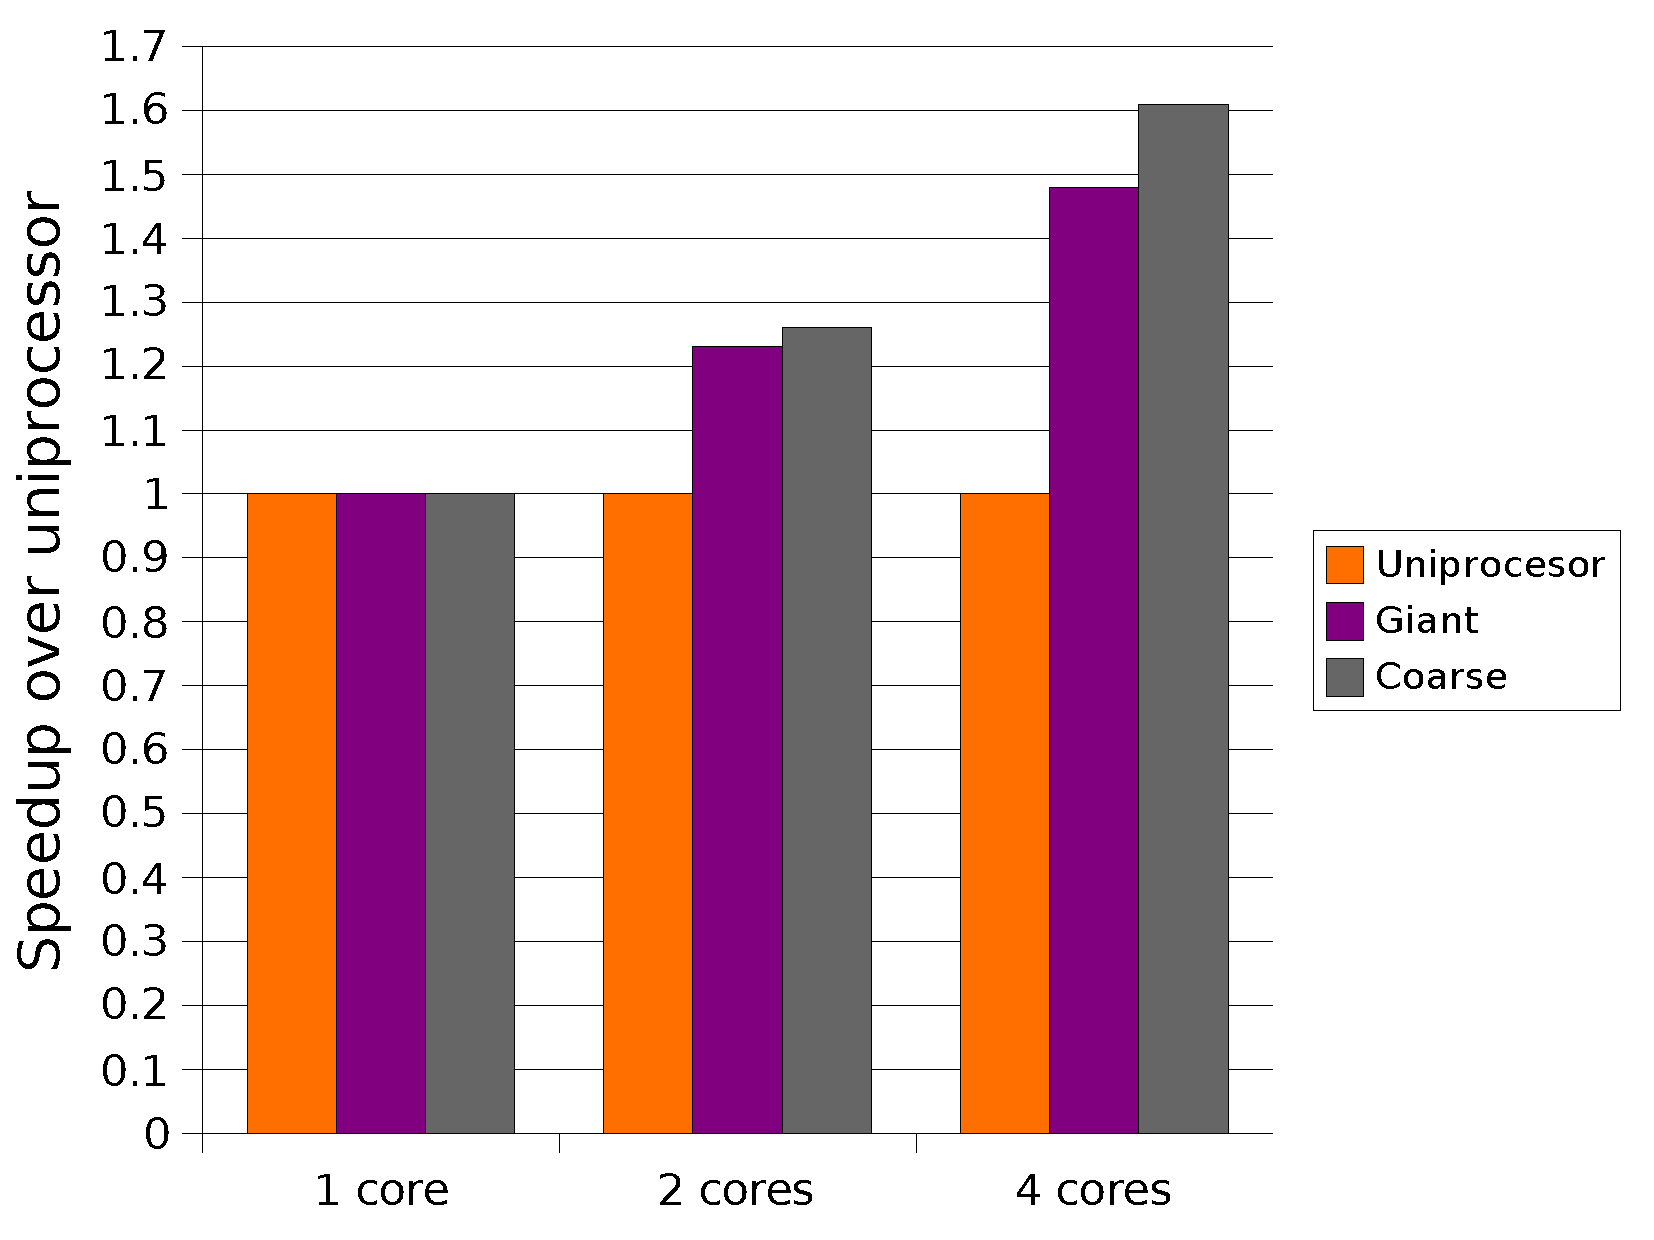
\includegraphics[width=0.8\linewidth]{figures/tsp-smp-coarse/refapp}
    \caption[C++ traffic performance results]{Performance results for the three kernel versions for C++ traffic.}
    \label{fig:dicos-cg:cpp-results}
  \end{center}
\end{figure}

\begin{figure*}[thb]
  \begin{center}
    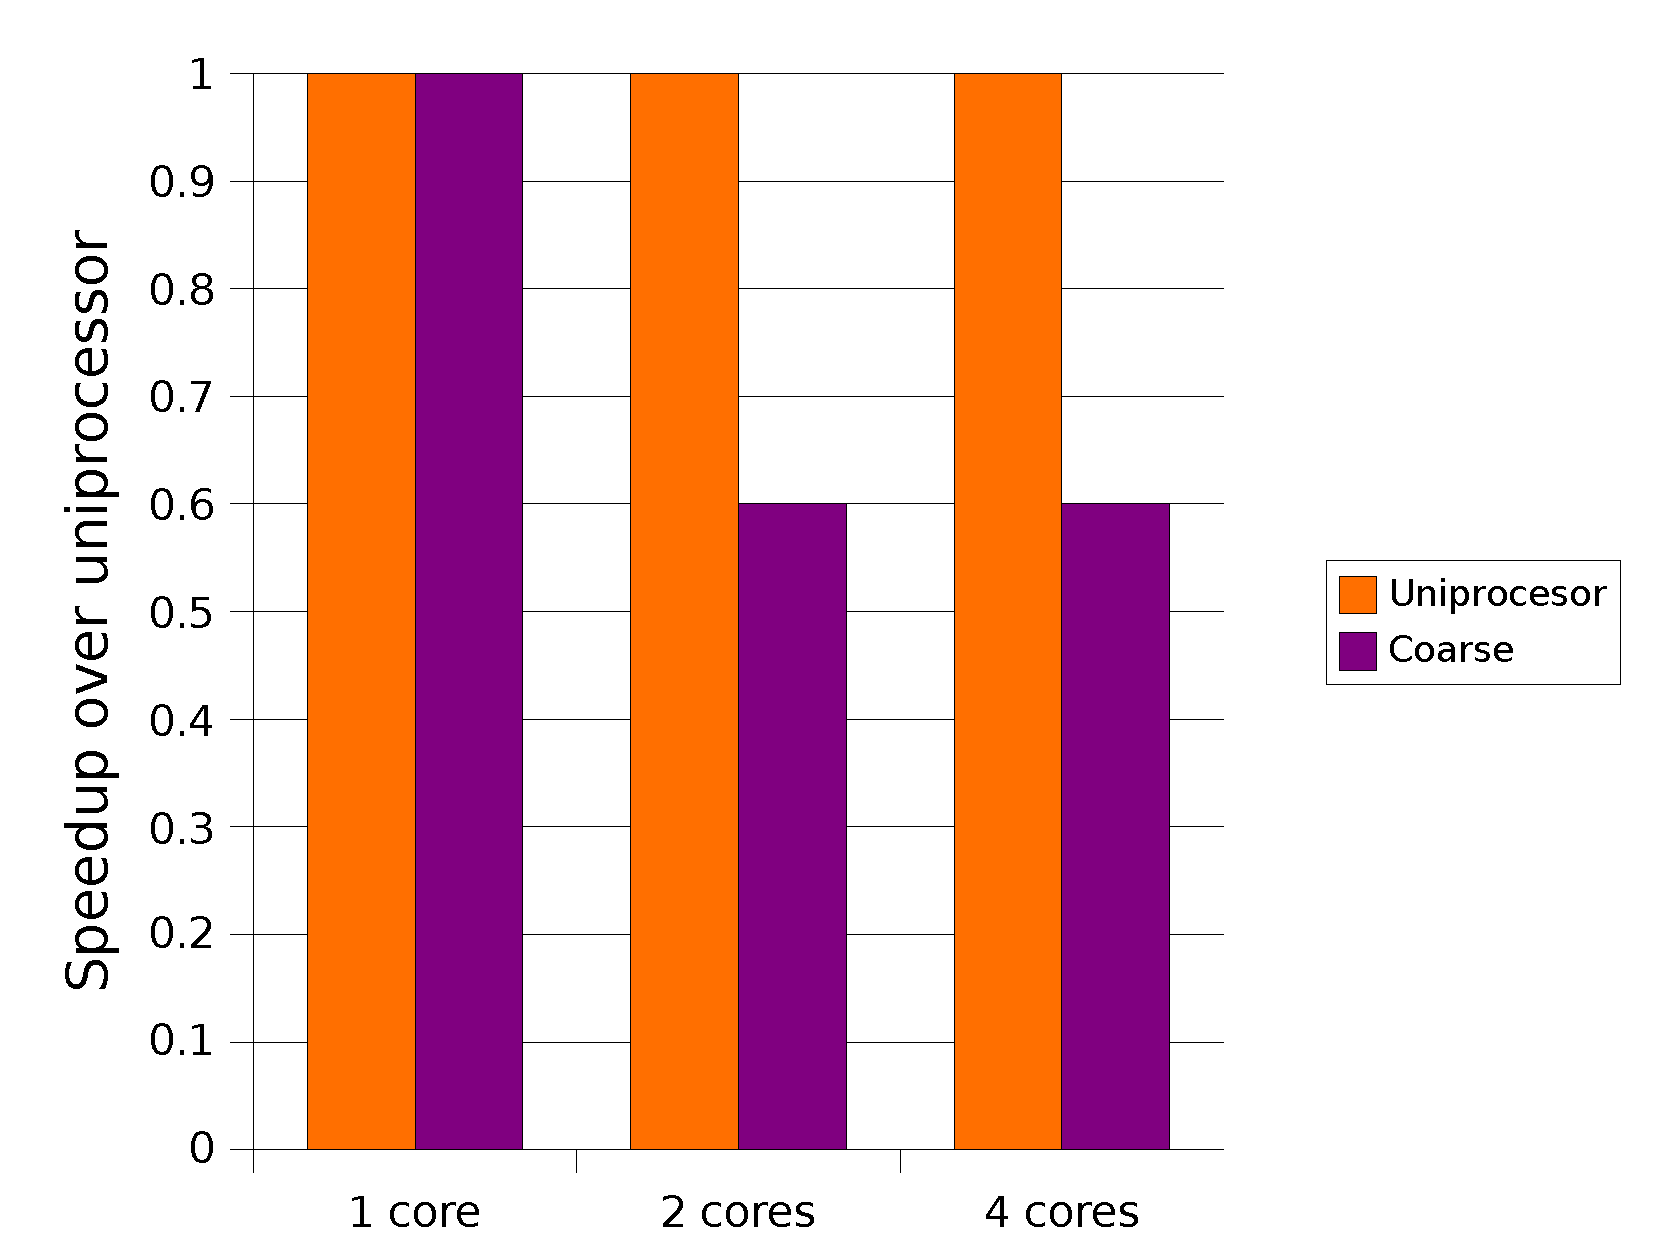
\includegraphics[width=0.6\linewidth]{figures/tsp-smp-coarse/java-no-lfh}~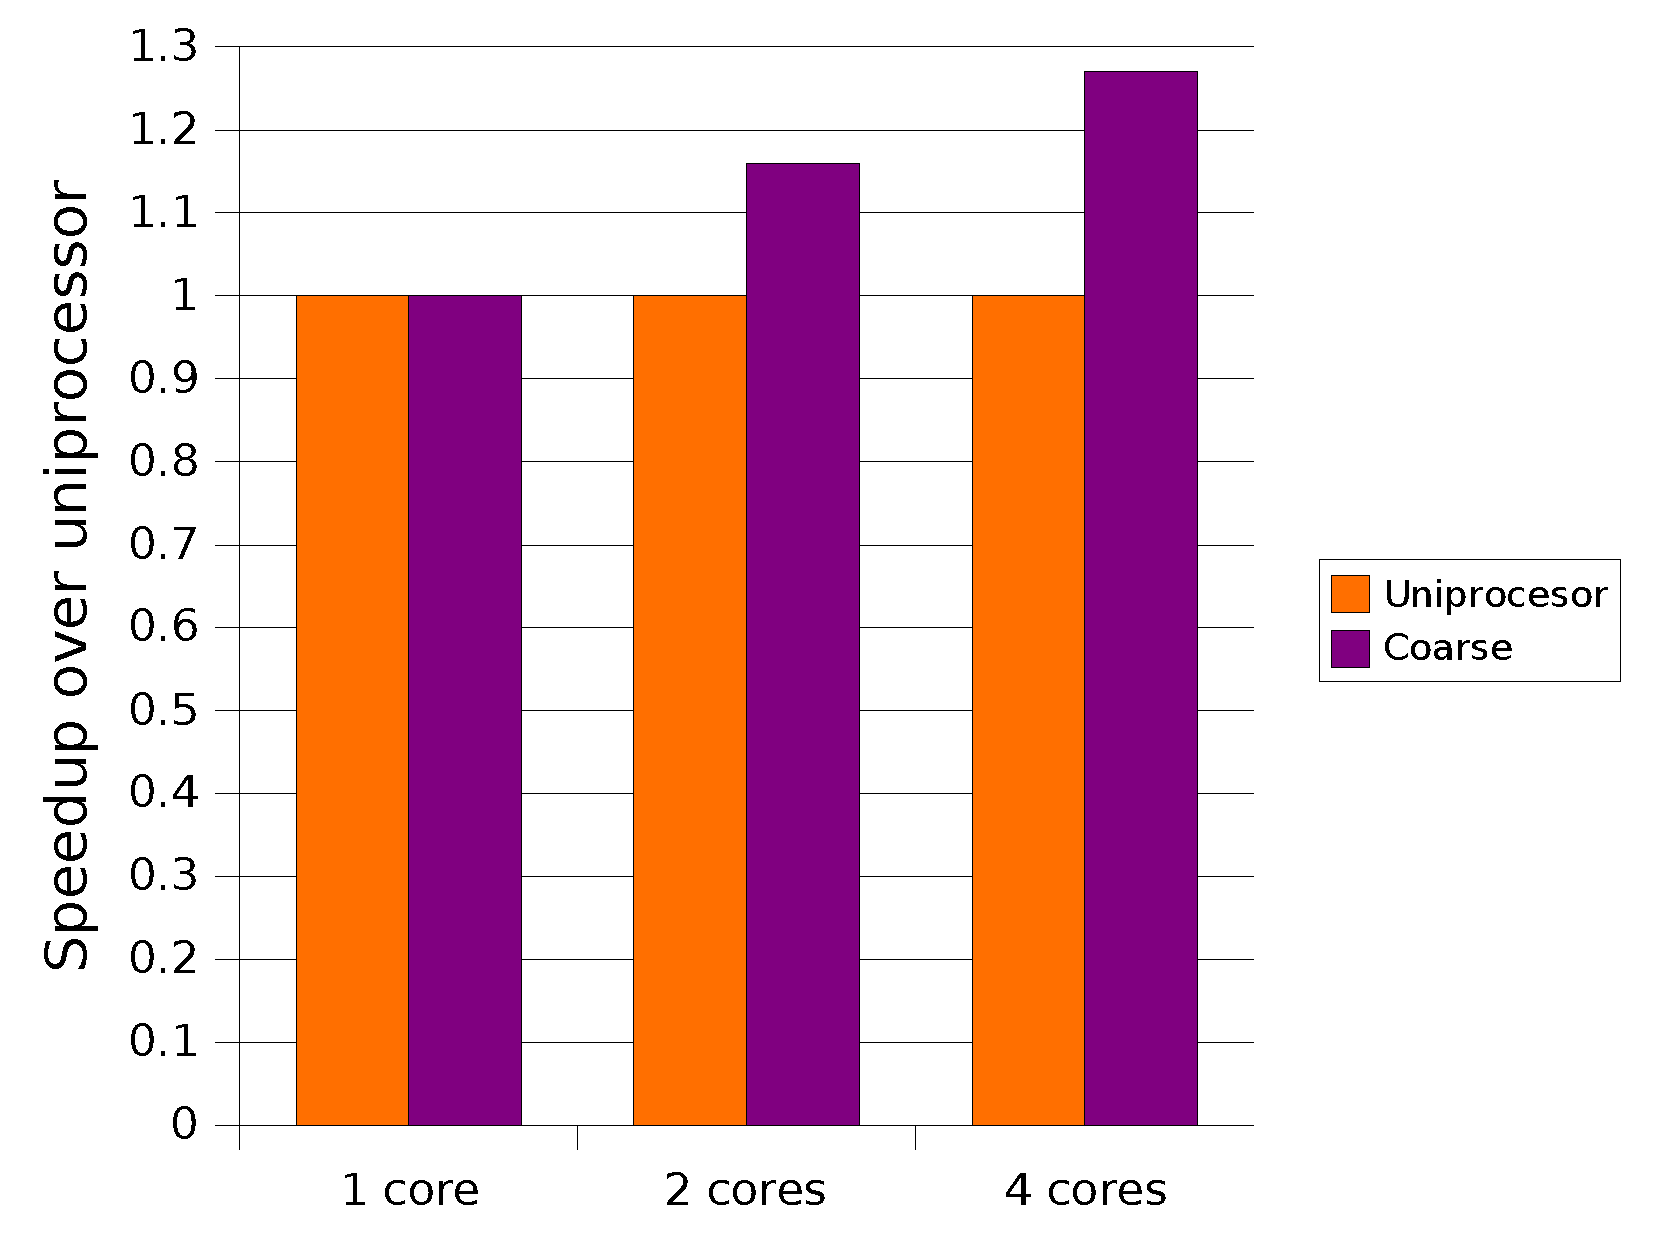
\includegraphics[width=0.6\linewidth]{figures/tsp-smp-coarse/java-lfh}
    \caption[Java traffic performance results]{Performance results for the three kernel versions for Java
      traffic. The left part of the figure shows the standard heap and the
      right shows the lock-free heap}
    \label{fig:dicos-cg:java-results}
  \end{center}
\end{figure*}

We measure at what level of calls per second the load of the system reaches
100\%, i.e., at what level the system cannot accept more work. The results are
anonymized and shows the speedup compared to uniprocessor operation. The test
runs with two kernels, one which holds the giant lock for all operations and
one which uses the coarse-grained locking implementation. The uniprocessor
version runs with all locks inactive, but contains the same memory management
implementation. The tests were performed on a 4-CPU machine with two dual-core
2.8GHz AMD Opterons.

The results for C++ traffic are shown in
Figure~\ref{fig:dicos-cg:cpp-results}. As the figure shows, the improvement
compared to the uniprocessor is around 20\% for the 2-core case with the giant
lock and 48\% for the 4-core case. For the coarse-grained locking, the
performance improvement compared to the uniprocessor is almost 23\% and 61\%
for the 2 and 4-core cases, which shows that the coarse-grained approach gives
some benefits over the pure giant lock. We expect that these numbers will
improve when the database has been separated to use it's own locks.

Figure~\ref{fig:dicos-cg:java-results} shows the results for Java traffic with
and without the lock-free heap for the uniprocessor and the coarse-grained
implementation. As the left part of the figure shows, the heap problems makes
performance deteriorate on multiprocessor configurations. Since threads are
almost always blocking on the heap semaphores, threads are effectively
serialized and multiple CPUs will only cause overhead. There is also no
scaling when going from two to four cores, which is also caused by the
serialized threads. The right part of the figure shows the results with the
lock-free heap. As can be seen in this figure, there is an improvement both in
the two- and four core cases, albeit not as much as with C++ traffic. The
results also scale between the two- and four core case. Again, we expect that
the performance will improve with the database lock.

\section{Related work}
\label{sec:dicos-cg:related}

The cluster-based operating system we are working with is perhaps most similar
to the Plurix operating system~\cite{goeckelmann03plurix}. Plurix is a
Java-based operating system which provides distributed shared memory with
communication through shared objects. The distributed in-RAM database in the
operating system serves a similar purpose, but is not implemented through
distributed shared memory. Also, the Plurix kernel only runs on uniprocessor
hardware and only supports a Java runtime environment whereas we support
multiprocessors and C++ as well and use a kernel written in C++.

There have been several ports of uniprocessor kernels targeting multiprocessor
systems. AIX~\cite{clark95symmetric, talbot95aix} was ported to multiprocessor
PowerPC hardware around 10 years ago. The port lasted around 18
months~\cite{talbot95aix} and totally involved more than 100 people, although
this includes other work for the next AIX release. Similar to our
implementation, the AIX developers used a mix between fine-grained and
coarse-grained locks, with some subsystems being locked by coarse-grained
locks and more performance critical ones using fine-grained locks. A
difference is the AIX kernel already allowed in-kernel thread preemption,
which means that the uniprocessor base already deals with some of the problems
we encountered. AIX locks can also block threads so that the CPU switches to
another thread. This is not possible in general with our kernel since it does
not allow kernel thread preemption.

Solaris~\cite{kleinman92solaris}, Linux~\cite{beck98linux},
FreeBSD~\cite{lehey03freebsd} have also been ported to multiprocessor systems.
For Linux and FreeBSD, the initial versions used a giant locking scheme
similar to our prototype. Their locking schemes have later been refined to
implement more fine-granular approaches, starting with coarse-grained locks
and gradually moving to fine-grained locking. The Solaris implementation
immediately moved to a fairly fine-grained locking approach.

The problem with heap allocators on multiprocessor platforms has been studied
in several earlier articles~\cite{haggander98icpp, haggander00pdcs,
  haggander99part, michael04pldi}. For applications which does frequent heap
allocations, introducing a multithreaded or lock-free heap can give
significant advantages. Our experience validates this observation and also
illustrates behavioral differences in multithreaded programs on uniprocessors
and multiprocessors.

There are also some alternative approaches to multiprocessor porting. For
example, the application kernel approach~\cite{kagstrom05appkern} describes a
method where a small \emph{application kernel} is installed as a loadable
module beside the regular kernel, and handles all CPUs except the boot CPU.
Applications thereafter run on the application kernel, but system calls are
forwarded to the boot CPU and handled by the original kernel. This approach
allows a multiprocessor port without changing the original kernel, but limits
scalability of kernel-bound work and is therefore unlikely to provide good
results for the operating system we are targeting. Virtualization is another
possible approach to benefit from a multiprocessor. Cellular
Disco~\cite{govil99cellular} partitions a large multiprocessor into a virtual
cluster, and runs multiple IRIX instances in parallel. However, virtualization
would require the high availability framework for the operating system to
change in order to avoid co-location of database objects on the same node. We
also investigated a port to the paravirtualized Xen system~\cite{barham03xen},
but for technical reasons it turned out to be difficult to implement.

\section{Conclusions}
\label{sec:dicos-cg:conclusions}
In this paper, we have described experiences from porting an operating system
kernel to multiprocessor hardware. We have outlined the implementation of
coarse-grained locking for the kernel, which is based on a prototype with a
giant lock that serializes kernel execution. We have also described the most
important problems which arose and our solutions to these. Our evaluation
shows that the coarse-grained approach improves on the giant locking approach
for the kernel-bound workload we target.

The prototype giant lock implementation has many similarities with the
uniprocessor implementation. Processes executing in the kernel are never
interrupted, so the original uniprocessor semantics are mostly kept
unmodified. The changes for the implementation were mostly related to CPU
startup and CPU-local data and the implementation of multithreaded address
spaces. After the initial implementation, correctness was therefore not a big
problem with the giant locking approach.

For the coarse-grained implementation, the changes to the uniprocessor base
are much larger. With multiple CPUs executing concurrently in the kernel, many
of the assumptions made in the uniprocessor implementation are no longer true.
While some of these problems were found and analyzed during the
prestudy-phase, e.g., the problems with multithreaded termination, others were
not found until we started prototyping the implementation. For example, we
first made the idle loop immediately enter the scheduler again to keep CPUs
busy, but since this was shown to cause a high contention on the giant lock we
revised the implementation. The heap locking problem, which actually occurs in
user-space, was similarly unexpected and was caused as an indirect effect of
true multithreading.

Our experiences illustrates the diversity of problems associated with
multiprocessor ports of operating system kernels. Since the changes affect
large parts of the code base, with parallelization of many parts of the
kernel, this type of port requires thorough knowledge of a large set of
modules in the kernel. In general, the difficult problems have occurred in
parts of the code that were not directly changed by the multiprocessor port.
For example, most of the timer code is not directly affected by the
multiprocessor port, yet it has caused several difficult indirect problems in
code that uses the timers.

While we've had a set of difficult problems during the implementation of the
coarse-grained locking approach, the duration of the project have still been
shorter than the giant lock prototype, which took almost two
years~\cite{kagstrom05experiences}. The primary reason is that the prototype
was implemented by a single developer without previous experience with the
operating system working part-time at a remote site, while the coarse-grained
approach was implemented by a team of experienced designers working on-site.
Another reason is simply that we could start from the already working giant
locking implementation and work incrementally from that, which has enabled the
development to continue in small steps. A third reason has been the improved
tool support, primarily the use of GDB through Qemu, which was not available
when the giant lock prototype was developed.

\section*{Acknowledgements}
This work was partly funded by The Knowledge Foundation in Sweden under a
research grant for the project ``Blekinge - Engineering Software Qualities
(BESQ)'' (\url{http://www.bth.se/~besq}).

%We would like to thank the anonymous reviewrs for their valuable input

%%% Local Variables: 
%%% mode: latex
%%% TeX-master: t
%%% End: 


\chapter{Paper~IV}
\papertitle{The Application Kernel Approach - a Novel Approach for Adding SMP Support to Uniprocessor Operating Systems}
  {Simon K�gstr�m, H�kan Grahn, Lars Lundberg}
  {Published in the Software: Practice and Experience Journal volume 36(13):1563--1583, November 2006}
\label{cha:paper4}
\label{cha:linux-appkern}
% Sw practice and experience.

\section{Introduction}
% From ipdps paper

For performance reasons, uniprocessor computers are now being replaced with
small multiprocessors. Moreover, modern processor chips from major processor
manufacturers often contain more than one CPU core, either logically through
Symmetric MultiThreading~\cite{eggers97simultaneous} or physically as a Chip
MultiProcessor~\cite{hammond97singlechip}.  For instance, current Intel
Pentium~4 and Xeon processors contain two logical
processors~\cite{marr02hyperthreading} and several other manufacturers are in
the process of introducing on-chip
multiprocessors~\cite{kahle99power4,spracklen05cmt}. With multiprocessors
becoming prevalent, good operating system support is crucial to benefit from
the increased computing capacity.

% Rewrite???
We are currently working on a project together with a major developer of
industrial systems. The company has over the last 10 years being developing an
operating system kernel for clusters of uniprocessor IA-32 computers. The
operating system has interesting properties such as fault tolerance and high
performance (mainly in terms of throughput). In order to take advantage of new
shared-memory multiprocessors, a multiprocessor version of the kernel is being
developed~\cite{kagstrom05experiences}.  However, we were faced with the
problem that it was very difficult and costly to make the needed modifications
because of the size of the code, the long time during which the code had been
developed (this has led to a code structure which is hard to grasp), and the
intricate nature of operating system kernels.

The situation described above illustrates the fact that making changes to
large software bodies can be very costly and time consuming, and there has
also been a surge of interest in alternative methods lately. For example, as
an alternative to altering operating system code, Arpaci-Dusseau et
al.~\cite{arpacidusseau01information} propose a method where ``gray-box''~
knowledge about algorithms and the behavior of an operating system are used to
acquire control and information over the operating system without explicit
interfaces or operating system modification. There has also been some work
where the kernel is changed to provide quality of service guarantees to large
unmodified applications~\cite{zhang03qos}.

For the kernel of our industrial partner, it turned out that the software
engineering problems when adding multiprocessor support were extremely difficult
and time-consuming to address using a traditional approach. Coupled to the
fact that the target hardware would not scale to a very large number of
processors during the foreseeable future (we expect systems in the range of 2
to 8 processors), this led us to think of another approach. In our approach,
we treat the existing kernel as a black box and build the multiprocessor
adaptations beside it. A custom kernel called \emph{the application kernel},
of which the original kernel is unaware, is constructed to run on the other
processors in the system while the original kernel continues to run on the
boot processor. Applications execute on the other processors while system
calls, page faults, etc., are redirected by the application kernel to the
uniprocessor kernel. We expect the application kernel approach to
substantially lower the development and maintenance costs compared to a
traditional multiprocessor port.

In this paper, we describe the application kernel approach and evaluate an
implementation for the Linux kernel. With this implementation, we demonstrate
that it is possible to implement our approach without changing the kernel
source code and at the same time running unmodified Linux applications. We
evaluate our approach both in terms of performance and implementation
complexity. The evaluation results show that the implementation complexity is
low in terms of lines of code and cyclomatic complexity for functions,
requiring only seven weeks to implement. Performance-wise, our implementation
performance-levels comparable to Linux for compute-bound applications.

The application kernel implementation for Linux is available as free software
licensed under the GNU General Public License (GPL) at
\url{http://www.ipd.bth.se/ska/application_kernel.html}. This paper builds on
our previous work where we implemented the application kernel approach for a
small in-house kernel~\cite{ska2004}.

The rest of the paper is structured as follows. We begin with discussing
related work in Section~\ref{sec:appkern:related_work}. In Section~\ref{sec:appkern:approach}
we describe the ideas behind our approach and Section~\ref{sec:appkern:implementation}
then discusses our implementation for the Linux kernel. We describe our
evaluation framework in Section~\ref{sec:appkern:evaluation_framework}, and then
evaluate the implementation complexity and performance of the application
kernel in Section~\ref{sec:appkern:results}.  Finally, we conclude and discuss future
extensions to the approach in Section~\ref{sec:appkern:conclusion}.


\section{Related Work}
\label{sec:appkern:related_work}
The implementation of a multiprocessor operating system kernel can be
structured in a number of ways.  In this section, we present the traditional
approaches to multiprocessor porting as well as some alternative methods and discuss
their relation to our approach.

\subsection{Monolithic Kernels}
Many multiprocessor operating systems have evolved from monolithic
uniprocessor kernels. These uniprocessor kernels (for example Linux and BSD
UNIX) contain large parts of the actual operating system, making
multiprocessor adaptation a complex task.  In-kernel data structures need to
be protected from concurrent access from multiple processors and this requires
locking. The granularity of the locks, i.e., the scope of the code or data
structures a lock protects, is an important component for the performance and
complexity of the operating system. Early multiprocessor operating systems
often used coarse-grained locking, for example the semaphore-based
multiprocessor version of UNIX described by Bach and
Buroff~\cite{bach84multiprocessor}\label{fix:bach}. These systems employ a
locking scheme where only one processor runs in the kernel (or in a kernel
subsystem) at a time~\cite{schimmel94unix}.  The main advantage with the
coarse-grained method is that most data structures of the kernel can remain
unprotected, and this simplifies the multiprocessor implementation. In the
most extreme case, a single ``giant''~lock protects the entire kernel.

The time spent in waiting for the kernel locks can be substantial for systems
dominated by in-kernel execution, and in many cases actually unnecessary since
the processors might use different paths through the kernel. The obvious
alternative is then to relax the locking scheme and use a more fine grained
locking scheme to allow several processors to execute in the kernel
concurrently.  Fine-grained systems allow for better scalability since
processes can run with less blocking on kernel-access.  However, they also
require more careful implementation, since more places in the kernel must be
locked.  The FreeBSD SMP implementation, which originally used coarse-grained
locking, has shifted toward a fine-grained method~\cite{lehey01freebsd} and
mature UNIX systems such as AIX and Solaris implement multiprocessor support
with fine-grained locking~\cite{clark95symmetric, kleinman92solaris}, as do
current versions of Linux~\cite{love2003linux}.

\subsection{Microkernel-based Systems}
Another approach is to run the operating system on top of a microkernel.
Microkernel-based systems potentially provide better system security by
isolating operating system components and also better portability since much
of the hardware dependencies can be abstracted away by the microkernel. There
are a number of operating systems based on microkernels, e.g.,
L4Linux~\cite{l4linux}, a modified Linux kernel which runs on top of the L4
microkernel~\cite{ukernelconstruction}. The Mach microkernel has been used as
the base for many operating systems, for example DEC~OSF/1~\cite{denham94osf1}
and MkLinux~\cite{mklinux}. Further, QNX~\cite{qnx} is a widely adopted
microkernel-based multiprocessor operating system for real-time tasks.
However, although the microkernel implements lower-level handling in the
system, a ported monolithic kernel still needs to provide locks around
critical areas of the system.

An alternative approach is used in multiserver operating systems~\cite{hurd,
  roscoeroscoestructure}. Multiserver systems organize the system as multiple
separated servers on a microkernel. These servers rely on microkernel
abstractions such as threads and address spaces, which can in principle be
backed by multiple processors transparently to the operating system servers.
However, adapting an existing kernel to run as a multiserver
system~\cite{gefflaut00sawmill, rawson97experience} requires major refactoring
of the kernel. Designing a system from scratch is a major undertaking, so in
most cases it is more feasible to port an existing kernel.


\subsection{Asymmetric Operating Systems}
\label{sec:appkern:related_asymetric}
Like systems which use coarse-grained locking, master-slave systems (refer to
Chapter 9 in~\cite{schimmel94unix}) allow only one processor in the kernel
at a time. The difference is that in master-slave systems, one processor is
dedicated to handling kernel operations (the ``master''~processor) whereas the
other processors (``slaves'') run user-level applications. On system calls and
other operations involving the kernel, master-slave systems divert the
execution to the master processor. Commonly, this is done through splitting
the ready queue into one slave queue and one master queue. Processes are then
enqueued in the master queue on kernel operations, and enqueued in the slave
queue again when the kernel operation finishes. Since all kernel access is
handled by one processor, this method limits throughput for kernel-bound
applications.

The master-slave approach is rarely used in current multiprocessor operating
systems, but was more common in early multiprocessor implementations. For
example, \label{fix:goble}Goble and Marsh~\cite{goble82dualvax} describe an
early tightly coupled VAX multiprocessor system, which was organized as a
master-slave system. The dual VAX system does not split the ready queue, but
instead lets the slave processor scan the ready queue for processes not
executing kernel code. Also, although both processors can be interrupted, all
interrupt handling (except timer interrupts) are done on the master processor.
Our approach is a modern refinement of the master-slave approach, where the
source code of the original system (``master'') remains unchanged.


% From SBAC-PAD paper
An interesting variation of multiprocessor kernels was presented in Steven
Muir's PhD. thesis~\cite{muir01piglet}\label{fix:muir}.
Piglet~\cite{muir01piglet} dedicates the processors to specific operating
system functionality.  Piglet allocates processors to run a Lightweight Device
Kernel (LDK), which normally handles access to hardware devices but can also
perform other tasks. The LDK is not interrupt-driven, but instead polls
devices and message buffers for incoming work. A prototype of Piglet has been
implemented to run beside Linux 2.0.30, where the network subsystem (including
device handling) has been off-loaded to the LDK, and the Linux kernel and
user-space processes communicate through lock-free message buffers with the
LDK. A similar approach has also been used to offload the TCP/IP stack
recently~\cite{regnier2004tcp}. These approaches are beneficial if
I/O-handling dominates the OS workload, whereas it is a disadvantage in
systems with much computational work when the processors would serve better as
computational processors. It can also require substantial modification of the
original kernel, including a full multiprocessor adaption when more than one
processor is running applications.

\subsection{Cluster-based Approaches}
% Make this sort of cluster-dependent
Several approaches based on virtualized clusters have also been presented. One
example is the Adeos Nanokernel~\cite{yaghmour2002} where a multiprocessor
acts as a cluster with each processor running a modified version of the Linux
kernel. The kernels cooperate in a virtual high-speed and low-latency network.
The Linux kernel in turn runs on top of a bare-bones kernel (the Adeos
nanokernel) and most features of Linux have been kept unchanged, including
scheduling, virtual memory, etc. This approach has also been used in
Xen~\cite{barham03xen}\label{fix:xen}, which virtualizes Linux or NetBSD
systems.

Another cluster-based method is Cellular Disco~\cite{govil99cellular}, where
virtualization is used to partition a large NUMA multiprocessor into a virtual
cluster which also provides fault-containment between the virtualized
operating systems. The virtualized systems provide characteristics similar to
our approach in that they avoid the complexity issues associated with a
traditional parallelization approach. However, they also require a different
programming model than single-computer systems for parallel applications.
Cluster-based approaches are also best suited for large-scale systems where
scalability and fault tolerance are hard to achieve using traditional
approaches.

MOSIX~\cite{mosix} is a single system image distributed system which redirects
system calls to the ``unique home node''~of the process, thereby utilizing the
central idea behind master-slave systems. MOSIX can distribute unmodified
Linux applications throughout a cluster of asymmetric hardware. MOSIX is
similar to our approach in that it redirects system calls, but has a different
goal (providing a single-system image distributed system).

\section{The Application Kernel Approach}

\label{sec:appkern:approach}
All of the approaches presented in the last section require, to various
degrees, extensive knowledge and modifications of the original kernel. We
therefore suggest a different approach, the \emph{application kernel
  approach}, which allows adding multiprocessor support with minimal effort
and only basic knowledge about the original kernel. In this section we
describe the general ideas behind the application kernel approach and an
overview of how it works.

\subsection{Terminology and Assumptions}
Throughout the paper, we assume that the implementation platform is the Intel
IA-32 although the approach is applicable to other architectures as well. We
will follow the Intel terminology when describing processors, i.e., the
processor booting the computer will be called the \emph{bootstrap processor}
while the other processors in the system are called \emph{application
  processors}.

Also, we use a similar naming scheme for the two kernels: the original
uniprocessor kernel is called the \emph{bootstrap kernel}, i.e., the Linux
kernel in the implementation described in this paper, whereas the second
kernel is called the \emph{application kernel}.  Further, in order to not
complicate the presentation, we will assume single-threaded processes in the
discussion, although multi-threaded processes are also supported using the
same technique.

\subsection{Overview}
The basic idea in our approach is to run the original uniprocessor kernel
\emph{as it is} on the bootstrap processor while all other processors run the
application kernel. Applications execute on both kernels, with the application
kernel handling the user-level part and the bootstrap kernel handling
kernel-level operations.  One way of describing the overall approach is that
the part of the application that needs to communicate with the kernel is
executed on a single bootstrap processor while the user-level part of the
program is distributed among the other processors in the system, i.e., similar
to master-slave kernels.

\begin{figure}
  \begin{center}
    \epsfig{width=0.6\linewidth, file=figures/linux-appkern/general_structure}
  \end{center}
  \caption{Overview of the application kernel approach.}
  \label{fig:approach}
\end{figure}

Figure~\ref{fig:approach} shows an overview of the application kernel
approach. The upper boxes represent user processes and the lower shows the
bootstrap kernel and the application kernel. Each process has two threads, a
\emph{bootstrap thread} and an \emph{application thread}. The bootstrap thread
executes on the bootstrap kernel, i.e., Linux, while the application threads
are handled by the application kernel. An application thread runs the actual
program code whereas the bootstrap thread serves as a proxy\label{fix:relay}
forwarding kernel calls to the bootstrap kernel. Note that the application
kernel and the bootstrap kernel use unique interrupt and trap handlers to
enable the application kernel to catch traps and faults caused by the
application.

The two threads in the process' communicate through a shared area in the
process address space. The bootstrap monitors the shared area to detect new
system calls etc. Applications run as before, except when performing
operations involving the kernel. On such events, the application thread traps
into the application kernel, which then enters a message in the communication
area. The actual event will be handled at a later stage by the bootstrap
thread, which performs the corresponding operation. We will describe trap
handling in detail in Section~\ref{sec:appkern:trap_handling}.

With the application kernel approach, we can add multiprocessor support to an
existing operating system without neither doing modifications to the original
operating system kernel, nor do we have to do any changes to the applications
(not even recompiling them). There are a few special cases that might require
kernel source changes, but those were not needed for our research prototype.
Section~\ref{sec:appkern:implementation_paging} describes these special cases.

Compared to the other porting methods, our approach tries to minimize the
effort needed to implement a multiprocessor port of a uniprocessor operating
system.  The focus is therefore different from traditional porting methods.
Master-slave kernels, which are arguably most similar to our approach, place
most of the additional complexity in the original kernel whereas we put it
into two separate entities (the application kernel and the bootstrap thread).
In a sense, our approach can be seen as a more general revitalization of the
master-slave idea. The Cache Kernel~\cite{greenwald96synergy,
  cheriton94caching} employs a scheme similar to ours on redirecting system
calls and page faults, but requires a complete reimplementation of the
original kernel to adapt it to the cache kernel. We can also compare it to the
MOSIX system~\cite{mosix} which also redirects system calls, although MOSIX is
used in a cluster context and has different goals then the application kernel.

\subsection{Hardware and Software Requirements}
The application kernel approach places some restrictions (often easy to
fulfill) on the processor architecture and the bootstrap kernel. The
architecture must support at least the following:

\begin{enumerate}
\item Binding of external interrupts to a specific processor and at the same
  time allow CPU-local timer interrupts.
\item Retrieving the physical page table address of the currently running
  process.
\item Interrupt and trap handlers must be CPU-local.
\end{enumerate}

The first requirement must be fulfilled since only the bootstrap kernel
handles all external interrupts except for timer interrupts. Timer interrupts
need to be CPU-local for scheduling to take place on the application kernel.
On the IA-32 this is possible to implement with the APIC (Advanced
Programmable Interrupt Controller), which has a per-processor timer.
\label{fix:local_timer}MIPS uses a timer in the coprocessor 0 on the processor
chip~\cite{mips01programmers} and PowerPC has a decrementer
register~\cite{ppcrefman} which can be used to issue interrupts.  The
interrupt \emph{handlers} must be private for different processors, which is
directly possible on IA-32 processors through the Interrupt Descriptor Table,
IDT. For architectures where the interrupt handlers reside on fixed addresses,
e.g., MIPS, instrumentation of the interrupt handlers are needed.

Our approach also places two requirements on the bootstrap kernel. First, it
must be possible to extend the kernel with code running in supervisor mode.
This requirement is satisfied in most operating systems, e.g., through
loadable modules in Linux. Second, the bootstrap kernel must not change or
remove any page mappings from the application kernel. The application kernel
memory needs to be mapped to physical memory at all times, since revoking a
page and handing it out to a process (or another location in the kernel) would
cause the application kernel to overwrite data for the bootstrap kernel or
processes.



\subsection{Application Kernel Interaction}
\label{sec:appkern:trap_handling}

Figure~\ref{fig:trap} shows how the kernel interaction works in the application
kernel approach. Kernel interaction requires 8 steps, which are illustrated in
the Figure. In the discussion, we assume that the operation is a system call,
although page faults and other operations are handled in the same way.

\begin{figure}
  \begin{center}
    \epsfig{width=0.6\linewidth, file=figures/linux-appkern/trap}
  \end{center}
  \caption[System call and trap handling]{System call/trap handling in the application kernel approach}
  \label{fig:trap}
\end{figure}

\begin{enumerate}
\item The application (i.e., the application thread running on one of the
  application processors) issues a system call and traps down to the
  application kernel. This is handled by the CPU-local trap vector.

\item The application kernel enters information about the call into the shared
  area, and thereafter schedules another thread for execution.
\item At a later point, the bootstrap thread wakes up and finds a message in
  the shared area.
\item The bootstrap thread then parses the message and performs the
  corresponding operation (i.e., issuing the same system call in this case).
\item The bootstrap kernel will thereafter handle the system call from the bootstrap
  thread and  return control to the bootstrap thread.
\item After this, the bootstrap thread must tell the application kernel that
  the application thread can be scheduled again. Since the application kernel
  runs as a loadable module within the bootstrap kernel, it must do this
  through the driver interface of the bootstrap kernel, issuing the
  application kernel \textbf{apkern\_activate\_thread} call.
\item The application kernel driver, running on the bootstrap processor,
  enters the application thread into the ready queue again.
\item Finally, the application thread is scheduled at a later point in time on
  one of the application processors.
\end{enumerate}

The \texttt{clone} and \texttt{fork} system calls are handled slightly
different then other calls, and are described in detail in
Section~\ref{sec:appkern:clone}.  Further, the \texttt{exit} system call and
exceptions that cause process termination (for example illegal instructions)
are different than page faults and other system calls. This is because the
bootstrap kernel is unaware of the application thread and will terminate the
process without notifying the application kernel. If this is not handled, the
application kernel will later schedule a thread which runs in a non-existing
address space. For this case, step 2 of the algorithm above is modified to
clean up the application thread (i.e., free the memory used by the thread
control block and remove the thread from any lists or queues).

Another special case is when the information flows the opposite way, i.e.,
when the kernel asynchronously activates a process (for instance in response
to a signal in Linux). In this case, the handler in the bootstrap thread will
issue the \textbf{apkern\_activate\_thread} call directly, passing information
about the operation through the shared area. The application kernel will then
issue the same signal to the application thread, activating it asynchronously.
\label{fix:signal_handlers}Our current implementation does not support
asynchronous notifications, but it would be achieved by registering signal
handlers during the bootstrap thread startup phase.


\subsection{Exported Application Programming Interface}
The application kernel API is only available via driver calls to the bootstrap
kernel. There is no way to call the application kernel directly via system
calls in the application thread since the trap handling matches that of the
bootstrap kernel and only forwards the events through the shared area. A
straightforward way of allowing direct calls to the application kernel would
be to use a different trap vector\label{fix:trap_vector} than the Linux
standard, which could be used e.g., to control application kernel scheduling
from applications. The exported interface consists of six calls:

\begin{itemize}
\item \textbf{apkern\_init}: This routine is called once on system startup,
  typically when the application kernel device driver is loaded. It performs
  the following tasks:
  \begin{itemize}
  \item It initializes data structures in the application kernel, for example the
    ready-queue structure and the thread lookup table.
  \item It starts the application processors in the system. On startup, each
    processor will initialize the interrupt vector to support system calls and
    exceptions. The processor will also enable paging and enter the idle
    thread waiting for timer interrupts.
  \end{itemize}
\item \textbf{apkern\_thread\_create}: This function is called from the
  bootstrap thread when the process is started. The function creates a new
  thread on the application kernel. The thread does not enter the ready queue
  until the \textbf{apkern\_thread\_start} call is invoked.

\item \textbf{apkern\_thread\_ex\_regs}: Sometimes it is necessary to update
  the register contents of a thread (for example copying the register contents
  from parent to child when forking a process), and the application kernel
  therefore has a call to ``exchange'' the register contents of a thread.

\item \textbf{apkern\_thread\_get\_regs}: This function returns in the current
  register context of a thread (also used with fork).

\item \textbf{apkern\_thread\_start}: Place a thread in the ready queue.

\item \textbf{apkern\_thread\_activate}: Thread activation is performed when
  the bootstrap thread returns, e.g., from a system call, to wake up the
  application thread again. The call will enter the application thread back
  into the ready queue and change its state from \emph{blocked} to
  \emph{ready}.
\end{itemize}



\section{Implementation}

\label{sec:appkern:implementation}

We implemented the application kernel as a loadable kernel module for Linux.
The module can be loaded at any time, i.e., the application kernel does not
need to be started during boot but can be added when it is needed. Since
modules can be loaded on demand, the application kernel can also be started
when the first process uses it. It is further not necessary to recompile
applications to run on the application kernel, and applications running on the
application kernel can coexist seamlessly with applications running only on
the bootstrap processor.

\label{fix:shared_area}The layout of the shared memory area for the Linux
implementation is shown in Figure~\ref{fig:shared_area}. The shared area data
type, \texttt{apkern\_comm\_entry\_t} has a union with the different types of
messages, with page faults and system calls shown in the figure and a variable
(\texttt{bootstrap\_has\_msg}) which is used by the application kernel to
signal to the bootstrap thread. There is always a one to one mapping between
application threads and bootstrap threads, i.e., multithreaded processes will
have several bootstrap thread. The bootstrap thread does not respond to system
calls etc., through the shared area, but invokes the application kernel driver
instead. Since the shared area is a one-way communication channel, it needs no
explicit protection.

\begin{figure}
  \footnotesize
  \begin{verbatim}
typedef struct {
  volatile bool_t bootstrap_has_msg;
  volatile apkern_comm_nr_t nr;
  volatile addr_t pc;

  union {
    struct {
      volatile addr_t addr;
      volatile bool_t write;
    } PACKED pagefault;

    struct {
      volatile uint_t nr;
      volatile uint_t arg1;
      ...
      volatile uint_t arg6;
      volatile uint_t ret;
    } PACKED syscall;
    ...
  } u;
} apkern_comm_entry_t;
  \end{verbatim}
  \caption{Shared area layout}
  \label{fig:shared_area}
\end{figure}

The application kernel is initialized, i.e., processors are booted etc., when
the kernel module is loaded. The application kernel is thereafter accessible
through a normal Linux device file, and a process that wants to run on the
application kernel opens the device file on startup and closes it when it
exits (this can be done automatically and is described in
\label{fix:forward_ref}Section~\ref{sec:appkern:running_applications}).  All interactions with the
application kernel, apart from \texttt{open} and \texttt{close}, are done
using \texttt{ioctl} calls, through which the exported interface is available.

\label{fix:device_driver}Figure~\ref{fig:driver_structure} illustrates the
application kernel driver (a char-type device) structure and an
\textbf{apkern\_activate\_thread} call. The call from the bootstrap thread
enters through the Linux system call handler which forwards it to the
\texttt{ioctl} entry point for the device driver. The \texttt{ioctl} handler
in turn updates the thread control block for the activated thread, locks the
application kernel ready queue, and enters the thread control block into the
ready queue. In the rest of this section, we will discuss details related to
paging, forking and application startup from the Linux implementation of the
application kernel.


\begin{figure}
  \begin{center}
    \epsfig{width=0.7\linewidth, file=figures/linux-appkern/driver_structure}
  \end{center}
  \caption{Application kernel device driver structure}
  \label{fig:driver_structure}
\end{figure}


\subsection{Paging}
% Paging
\label{sec:appkern:implementation_paging}

All page faults are handled in the bootstrap thread by setting the stack
pointer to the address of the page fault and touching that memory area.
Although this seems like an unnecessary step instead of just accessing the
memory directly, it is needed as a workaround since Linux terminates the
program if stack access is done below the current stack pointer.

The paging implementation also illustrates the one case where the application
kernel approach might require kernel modifications. The problem (which is
general and affects other approaches as well) occurs in multi-threaded
processes on page table updates, when the translation lookaside buffer (TLB)
contents for different processors running in the same address space will be
inconsistent\footnote{On architectures with tagged TLBs, e.g., MIPS, this
  could occur even in single-threaded processes since the TLB is not
  necessarily flushed on page table switches.}. For example, if processor 0
and 1 execute threads in the same address space, and processor 0 revokes a
page mapping, the TLB of processor 1 will contain an incorrect cached
translation. To solve this, an inter-processor interrupt is invoked to
invalidate the TLB of the other processors, which requires changes to the page
fault handling code. In our prototype, we ran without disk swap and the
inter-processor interrupts are therefore not needed and have not been
implemented.

% clone
\subsection{\texttt{clone}/\texttt{fork} System Calls}
\label{sec:appkern:clone}
The Linux \texttt{clone} and \texttt{fork} system calls require special
handling in the application kernel. Both calls start a new process which
inherits the context of the invoking thread. The difference is that
\texttt{clone} allows for sharing the address space with the parent (creating
a new thread), while \texttt{fork} always separate the address spaces
(creating a new process).  \texttt{clone} also requires the invoker to specify
a callback function that will be executed by the cloned thread.  In Linux,
\texttt{fork} is simply a special case of \texttt{clone},
\label{fix:clone}although the implementation of \texttt{fork} predates
\texttt{clone}.

We illustrate the steps needed in a \texttt{clone} or \texttt{fork} call in
Figure~\ref{fig:clone}. If we would just issue the system call directly, the
bootstrap thread would run the cloned thread itself. Therefore we first clone
the bootstrap thread, then let the cloned bootstrap thread create a new
application kernel thread (i.e., handling the original clone), and finally
enters a loop waiting for messages from the application kernel. This
effectively splits the \texttt{clone} call in two, creating a new thread pair.
The \texttt{fork} call works the same way, but has different return semantics,
i.e., it returns ``twice''~instead of using a callback.

\begin{figure}
  \begin{center}
    \epsfig{width=0.7\linewidth, file=figures/linux-appkern/fork}
  \end{center}
  \caption{Handling of the \texttt{clone} system call}
  \label{fig:clone}
\end{figure}

\subsection{Running Applications}
\label{sec:appkern:running_applications}
Our implementation allows running dynamically linked applications directly,
without modifying or even recompiling them. It is also possible to run a mixed
system, with some applications running on the application kernel whereas
others are tied to the bootstrap processor.

We achieve this by applying some knowledge about application startup under
Linux. In Linux, applications are started by a short assembly stub which in
turn calls \texttt{\_\_libc\_start\_main}. This function, provided by GNU
libc, starts the \texttt{main} function.  The \texttt{\_\_libc\_start\_main}
function is dynamically linked into the executable and can therefore be
overridden. We override \texttt{\_\_libc\_start\_main} with the startup
routine for the application kernel, which can be done as long as the
application is dynamically linked against libc. To run a process on the
application kernel, we simply set the \texttt{LD\_PRELOAD} environment
variable to preload a library with the bootstrap thread implementation.

\begin{figure}
  \begin{center}
    \epsfig{width=0.7\linewidth, file=figures/linux-appkern/app_startup}
  \end{center}
  \caption[Application startup]{Application startup. The dashed lines shows the original execution
    while the solid lines show the overridden execution path.}
  \label{fig:start_main_override}
\end{figure}

The overriding process is illustrated in Figure~\ref{fig:start_main_override}.
The overridden \texttt{\_\_libc\_start\_main} will just invoke the original
\texttt{\_\_libc\_start\_main}, but with \texttt{apkern\_thread} instead of
\texttt{main} as starting function. This function in turn will either,
depending on if the \texttt{NOAPPKERN} environment variable is set, invoke the
original \texttt{main} and thereby bypassing the application kernel, or start
the bootstrap thread.


\section{Experimental Setup and Methodology}
\label{sec:appkern:evaluation_framework}
We have conducted an evaluation of the application kernel approach where we
evaluate both latency and throughput. First, we measure single-process
performance in order to estimate the extra latency caused by the application
kernel. Second, we measure scalability of multiprogramming and parallel
benchmarks. In the evaluation, we use standard UNIX tools, the
SPLASH~2~\cite{cameron95splash} benchmarks and the SPEC
CPU2000~\cite{spec2000} benchmark suite. Further, we have also evaluated the
implementation size and complexity of our approach, which was performed by
counting the physical lines of code in the application kernel and calculating
the McCabe cyclomatic complexity~\cite{fenton98swmetrics} which gives the
number of independent code paths through a function. The code lines were counted
with the sloccount tool~\cite{sloccount} by David A. Wheeler and the cyclomatic
complexity was measured by the pmccabe tool by Paul Bame~\cite{pmccabe}.

\subsection{Evaluation Environment}

We performed our performance evaluation using the Simics full system
simulator~\cite{simics} and real hardware. We setup Simics to simulate a
complete IA-32 system with 1 to 8 processors. Our hardware is a 200MHz dual
Pentium Pro with 8KB first-level instruction and data caches, and a 256KB
per-processor L2 cache. The Simics simulator allows us to use unmodified hard
disk images, containing the complete operating system.  Compared to real
hardware, our simulated setup does not simulate caches in the system, and some
other performance issues relevant in multiprocessor
systems~\cite{gamsa95performance}, such as costs associated with data
alignment, cross-processor cache access etc., are not accounted for in our
simulations. Our prototype also has known performance issues, e.g., we have
not optimized the memory layout for efficient use of the cache. However, the
fundamental limitation of the application kernel approach is that the
bootstrap thread at some point will be a scalability bottleneck. We believe
that the simulated measurements give a good indication of when this bottleneck
is reached for various usage patterns.

\label{fix:hardware}The execution on hardware serves to validate the correctness of our
implementation in a real setting, and is also used to establish the latency
for kernel operations with the application kernel. We successfully ran all the
benchmarks on our hardware as well as on the simulated system.

We benchmarked uniprocessor Linux with the application kernel module against
multiprocessor Linux, running the 2.4.26 version of the kernel, henceforth
referred to as SMP Linux. Our experiments report the time required to execute the
benchmarks in terms of clock cycles on the bootstrap processor. Our system was
a minimal Debian GNU/Linux 3.1 (``Sarge'')-based distribution, which ran
nothing but the benchmark applications.

\begin{table}
  \caption{The benchmarks used in the performance evaluation}
  \begin{center}
    \begin{small}
      \label{tab:benchmarks}
      \begin{tabular}{p{2.6cm}|l|p{4.2cm}}
        Benchmark & Command & Description \\
        \hline
        \multicolumn{3}{l}{} \\
        \multicolumn{3}{l}{\textbf{Single-process benchmarks}} \\
        \hline
        find & \texttt{find /} & List all files in the system (13,946 files and directories) \\
        \hline
        SPEC2000 gzip & \texttt{164.gzip lgred.log} & Compression of a logfile,
        computationally intensive. \\
        \hline
        SPEC2000 gcc & \texttt{176.gcc smred.c-iterate.i} & SPEC 2000 C-compiler. \\
        & \texttt{-o a.s} \\
        \hline
        \multicolumn{3}{l}{} \\
        \multicolumn{3}{l}{\textbf{Parallel benchmarks}} \\
        \hline
        SPLASH2 RADIX & \texttt{RADIX -n 8000000 -p8} & Sort an array with radix
        sort, 8 threads.\\
        \hline
        SPLASH2 FFT & \texttt{FFT -m20 -p8} & Fourier transform, 8 threads. \\
        \hline
        SPLASH2 LU (non-contiguous) & \texttt{LU -p 8 -b 16 -n 512} & Matrix
        factorization, 8 threads. \\
        \hline
        \multicolumn{3}{l}{} \\
        \multicolumn{3}{l}{\textbf{Multiprogramming benchmarks}} \\
        \hline
        176.gcc & \texttt{176.gcc smred.c-iterate.i} & SPEC2000 C-compiler \\
        & \texttt{-o a.s} \\
        \hline
        find & \texttt{find /} & List all files in the system (13,946 files and
        directories). \\
        \hline
        grep & \texttt{grep "linux" System.map} & Search for an expression
        in a file. System.map has 150,000 lines. \\
        \hline
        find and grep & \texttt{find / | grep "data"} & List all files in the
        system and search for a string in the results.\\
        \hline
        SPLASH2 FFT & \texttt{FFT -m10 -p8} & Fourier transform, 8 threads. \\
        \hline
        SPLASH2 LU & \texttt{LU -p 8 -b 16 -n 512} &
        Matrix factorization, 8 threads. \\
      \end{tabular}
    \end{small}
  \end{center}
\end{table}

\subsection{Benchmarks}
For the performance evaluation, we conducted three types of performance
measurements. First, we ran a number of single-process benchmarks to evaluate
the overhead caused by the system call forwarding used by the application
kernel approach. These benchmarks run one single-threaded process at a time
and should therefore be unaffected by the number of processors. Second, we
also ran a set of multithreaded parallel applications, which shows the
scalability of compute-bound applications. Third, we also evaluated a
multiprogramming workload. In the multiprogramming benchmark, we ran a set of
programs concurrently and measured the duration until the last program
finished. This benchmark should be characteristic of a loaded multi-user
system.

The programs we used are a subset of the SPEC CPU2000 benchmarks, a subset of
the Stanford SPLASH 2 benchmarks, and a set of standard UNIX tools. For SPEC
CPU2000, we used the Minnespec reduced workloads~\cite{minnespec} to provide
reasonable execution times in our simulated environment. The SPLASH 2
benchmarks were compiled with a macro package which uses \texttt{clone} for
the threading implementation and pthread primitives for mutual exclusion. The
SPLASH SPEC benchmarks were compiled with GCC version 3.3.4 (with optimization
-O2) and the UNIX applications were unmodified Debian binaries. The benchmark
applications are summarized in Table~\ref{tab:benchmarks}.

\section{Experimental Results}
\label{sec:appkern:results}
In this Section, we describe the results obtained from our measurements.
Table~\ref{tab:single_process} and \ref{tab:parallel} show the speedup vs.
uniprocessor Linux for SMP Linux and the application kernel. For the parallel
and multiprogramming benchmarks, the speedup is also shown in
Figure~\ref{fig:parallel}. The results from the \texttt{getpid} evaluation is
shown in Table~\ref{tab:getpid}.


\subsection{Performance Evaluation}
\begin{table}
  \caption{\texttt{getpid} latency in Linux and the application kernel}
  \begin{center}
    \label{tab:getpid}
    \begin{small}
      \begin{tabular}{l|rr}
        & Linux & Application Kernel \\
        \hline
        PPro 200MHz & 970 & 5,700 \\
        Simics & 74 & 860 \\
      \end{tabular}
    \end{small}
  \end{center}
\end{table}

\label{fix:lmbench}On our hardware, issuing a \texttt{getpid} call takes
around 970 cycles in Linux on average (the value fluctuates between 850 and
1,100 cycles) whereas the same call requires around 5,700 cycles with the
application kernel as shown in Table~\ref{tab:getpid}.  In Simics, the cost of
performing a \texttt{getpid} call is 74 cycles in Linux and around 860 cycles
with the application kernel. Since \texttt{getpid} performs very little
in-kernel work, the cost for Linux is dominated by the two privilege level
switches (user mode to kernel and back). For the application kernel, there are
five privilege level switches (see Figure~\ref{fig:trap}). First, the
application thread traps down into the application kernel, which updates the
shared area. The bootstrap thread thereafter performs another trap for the
actual call and upon return invokes the application kernel driver through an
\texttt{ioctl} call, i.e., performing another three privilege level switches.
Finally, the application thread is scheduled again, performing the fifth
privilege level switch. In our simulated system, each instruction executes in
one cycle and there is no additional penalty for changing privilege mode and
therefore the \texttt{getpid} cost is dominated by the number of executed
instructions.  This explains why the application kernel overhead is
proportionally larger in the simulated system than on real hardware.

\begin{table*}
  \caption[Single-process speedup]{Speedup for the single-process benchmarks.}
  \begin{center}
    \label{tab:single_process}
    \begin{footnotesize}
      \begin{tabular}{r|rr|rr|rr}
        \hline
        & \multicolumn{6}{c}{Speedup vs. uniprocessor Linux} \\
        & \multicolumn{2}{c}{Find} & \multicolumn{2}{c}{176.gcc} & \multicolumn{2}{c}{164.gzip} \\
        CPUs & Linux & Appkern  & Linux & Appkern  & Linux & Appkern \\
        \hline
        % Find                    176.gcc           164.gzip
2 & 0.9803 & 0.7844 & 1.0015 & 0.8976 & 1.0008 & 0.9461 \\
3 & 0.9795 & 0.8284 & 1.0033 & 0.9125 & 1.0012 & 0.9461 \\
4 & 0.9807 & 0.8641 & 1.0047 & 0.9218 & 1.0014 & 0.9462 \\
5 & 0.9804 & 0.8690 & 1.0053 & 0.9230 & 1.0016 & 0.9462 \\
6 & 0.9800 & 0.8748 & 1.0047 & 0.9244 & 1.0016 & 0.9462 \\
7 & 0.9795 & 0.8784 & 1.0050 & 0.9252 & 1.0017 & 0.9462 \\
8 & 0.9776 & 0.8831 & 1.0055 & 0.9260 & 1.0017 & 0.9462 \\

        \hline
      \end{tabular}
    \end{footnotesize}
  \end{center}
\end{table*}

In the computationally intensive single-process \texttt{gcc} and \texttt{gzip}
benchmarks from SPEC CPU2000, the application kernel performs almost on-par
with SMP Linux (the difference is between 5 and 10\%) as shown in
Table~\ref{tab:single_process}.  Further, we can also see that as more
processors are added, the gap decreases because there is a higher probability
of a processor being free to schedule the thread when the bootstrap thread has
handled the call.

A weak spot for the application kernel shows in the filesystem-intensive
\texttt{find} benchmark. Here, the overhead associated with forwarding system
calls prohibit the application kernel to reach SMP Linux performance levels.
However, since application kernel applications can coexist seamlessly with
applications tied to the bootstrap kernel, it is easy to schedule these
applications on the bootstrap kernel.

\begin{table*}
  \caption[Parallel and multiprogramming speedup]{Speedup for the parallel and multiprogramming benchmarks.}
  \begin{center}
    \label{tab:parallel}
    \begin{footnotesize}
      \begin{tabular}{r|rr|rr|rr|rr}
        \hline
        & \multicolumn{6}{c}{Speedup vs uniprocessor Linux} \\
        & \multicolumn{2}{c}{RADIX} & \multicolumn{2}{c}{FFT} & \multicolumn{2}{c}{LU} & \multicolumn{2}{c}{Multiprogramming} \\
        CPUs & Linux & Appkern  & Linux & Appkern  & Linux & Appkern & Linux & Appkern\\
        \hline
        2 & 2.0433 & 1.0834& 1.6916 & 1.0401 & 1.9217 & 1.2662 & 1.5049 & 0.9705 \\
3 & 3.3758 & 2.5174& 2.2930 & 1.8654 & 2.9430 & 2.0795 & 1.6627 & 1.1375 \\
4 & 4.0885 & 3.7227& 2.5090 & 2.3235 & 3.5053 & 2.9941 & 1.6850 & 1.1779 \\
5 & 5.1898 & 4.8200& 2.8456 & 2.6323 & 4.0857 & 3.8009 & 1.6782 & 1.1878 \\
6 & 5.9562 & 5.5736& 2.9927 & 2.8626 & 4.7706 & 5.0445 & 1.6845 & 1.1962 \\
7 & 6.9355 & 6.1934& 3.1732 & 3.0188 & 5.3277 & 5.1628 & 1.6803 & 1.2059 \\
8 & 8.0009 & 6.0924& 3.3272 & 3.0745 & 6.0084 &        & 1.6839 &        \\

        \hline
      \end{tabular}
    \end{footnotesize}
  \end{center}
\end{table*}

The selected computationally intensive parallel benchmarks from the Stanford
SPLASH 2 suite exhibit good scalability both in SMP Linux and for the
application kernel (see Table~\ref{tab:parallel} and
Figure~\ref{fig:parallel}). The results for the application kernel are close
to those for SMP Linux, especially considering that the application kernel
excludes one of the processors (the bootstrap processor) for computation. This
shows that the application kernel is a feasible approach for computationally
intensive applications, where the kernel interaction is limited.

\begin{figure*}
  \caption[Speedup vs uniprocessor Linux]{Speedup for the parallel and multiprogramming benchmarks vs.
    uniprocessor Linux.}
  \begin{center}
    \begin{small}
      \begin{tabular}{cc}
        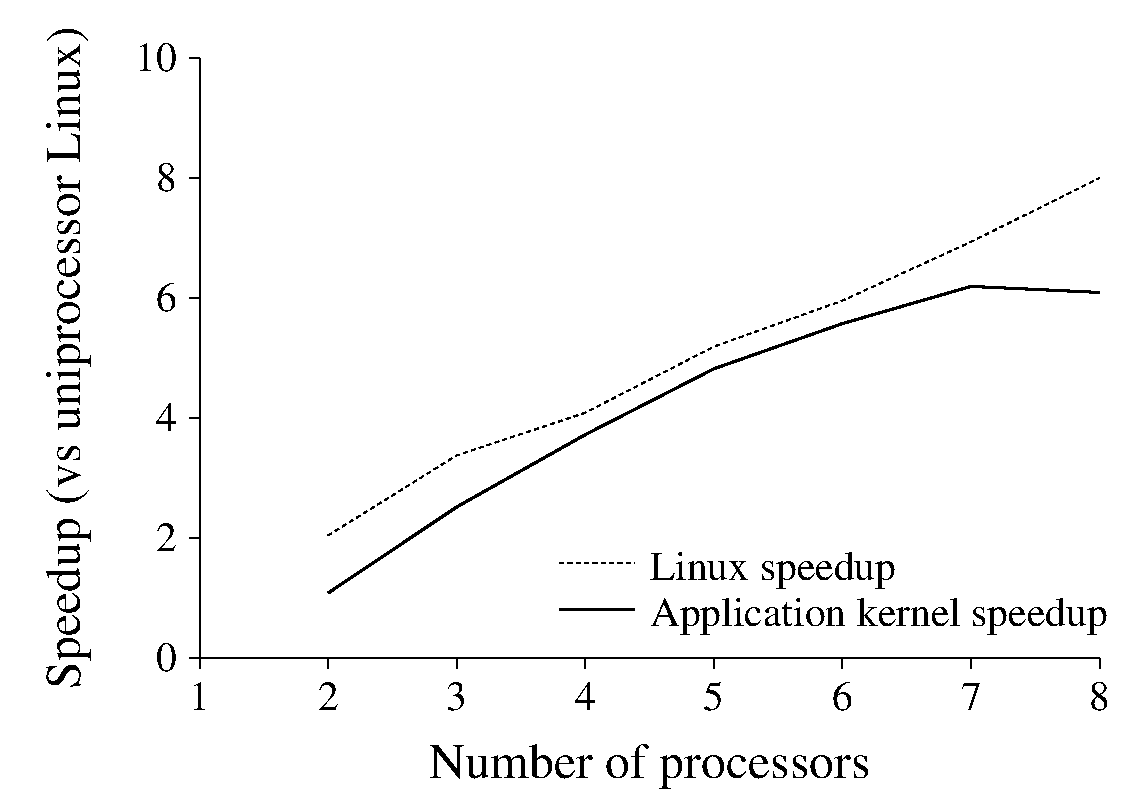
\epsfig{width=0.44\linewidth, file=./data/linux-appkern/RADIX_p8}\hspace{1.0cm} & 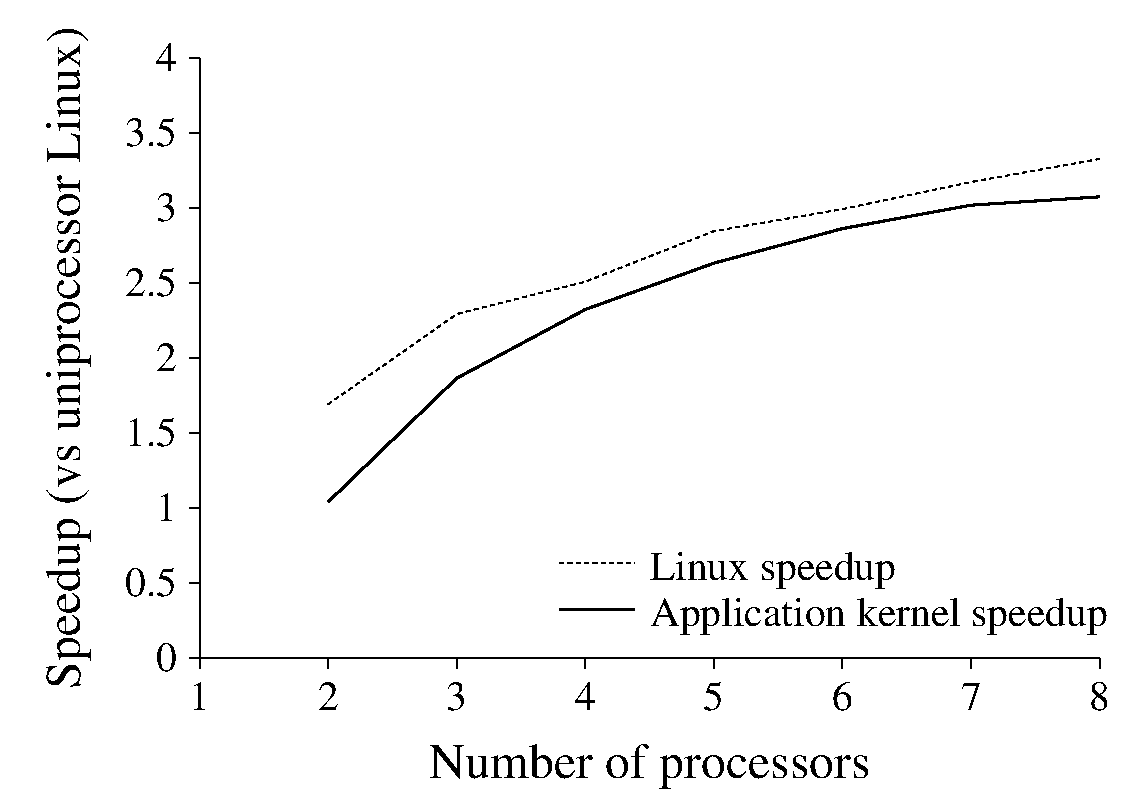
\epsfig{width=0.44\linewidth, file=./data/linux-appkern/FFT_p8}\\
        RADIX & FFT \\
        \vspace{0.1cm}
        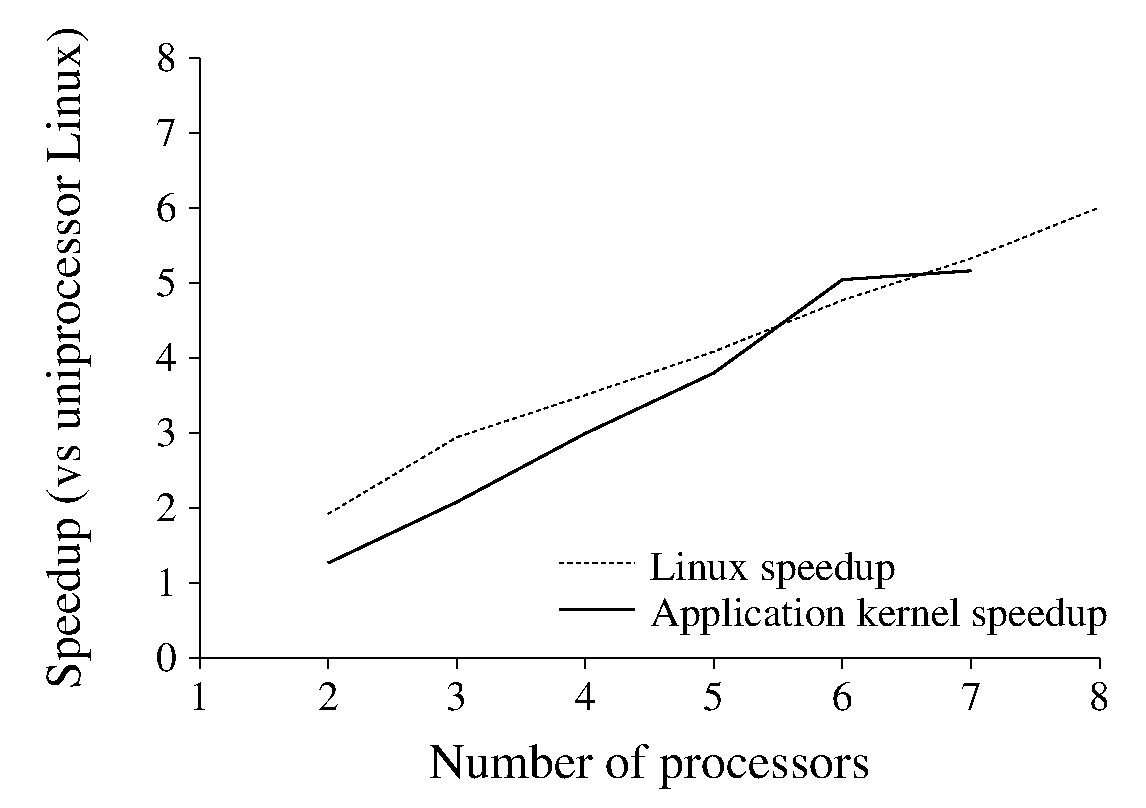
\epsfig{width=0.44\linewidth, file=./data/linux-appkern/lu_non_cont}\hspace{1.0cm} & 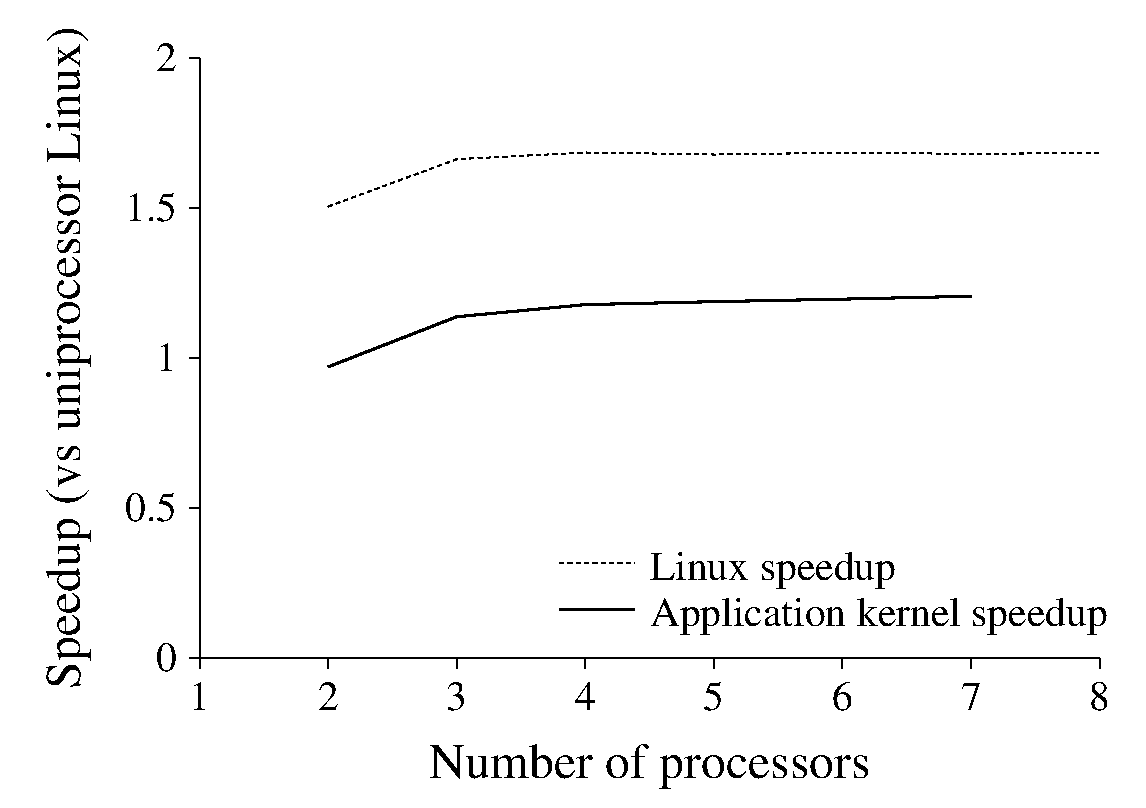
\epsfig{width=0.44\linewidth, file=./data/linux-appkern/multiprogramming}\\
        LU & Multiprogramming \\
      \end{tabular}
    \end{small}
    \end{center}
  \label{fig:parallel}
\end{figure*}

The multiprogramming benchmark, also shown in Table~\ref{tab:parallel} and
Figure~\ref{fig:parallel}, contains a mix of applications which have different
behavior in terms of user/kernel execution. For this benchmark, we see that
running all applications on the application kernel places a high strain on the
bootstrap kernel, which hampers the scalability compared to SMP Linux. For
general multiprogramming situations, it is probably better to divide the
processes so that kernel-bound processes run on the bootstrap processor while
the rest are executed on the application kernel.

\subsection{Implementation Complexity and Size}
The application kernel was ported from the implementation presented
in~\cite{ska2004}, and most of the internals of the kernel are completely
unchanged. Apart from some restructuring and the loadable Linux kernel module,
the only changes to the actual application kernel is some low-level handling
of system calls (i.e., the used trap vector and parameter passing).
One single developer spent seven weeks part-time implementing the application
kernel support for Linux. The previous implementation took about five
weeks to finish, and was also done by a single developer.

The number of physical code lines (not counting empty and comments) in
the application kernel is 3,600. Of these, the Linux driver module takes up
around 250 lines, roughly equally split in initialization and handling of
\texttt{ioctl} calls. Only around 400 lines of the implementation were changed
from our previous implementation. Libraries, a small part of libc and
malloc, list, stack and hash table implementations, account for another 920
lines of code.  The user-level library which contains the bootstrap thread
consists of 260 lines of code. Roughly one third of these are needed for the
handling of \texttt{clone} and \texttt{fork} while around 70 lines are needed
for startup.  The rest is used in the implementation of page fault and system
call handling (excluding \texttt{clone} and \texttt{fork}). The code lines are
summarized in Table~\ref{tab:loc}.

\begin{table}
  \caption{Comment-free lines of code}
  \begin{center}
    \vspace{0.2cm}
    \label{tab:loc}
    \begin{small}
      \begin{tabular}{l|r}
        Category & Lines of code \\
        \hline
        Application kernel & 2,400 \\
        Linux driver & 360 \\
        Libraries  & 920 \\
        Bootstrap thread & 260 \\
      \end{tabular}
    \end{small}
  \end{center}
\end{table}

The source consists of around 360 lines of assembly code and the rest being
C-code. The high proportion of assembly code, almost 10\%, stems from the fact
that a fairly large part of the code deals with startup of the application
processors and low-level interrupt handling. If we disregard the library code
(which is independent of the application kernel), the assembly portion
increases to 17\%.

\label{fix:mccabe}A histogram of the McCabe cyclomatic complexity for the
application kernel (without the library implementation), and the kernel core
and the IA-32-specific parts of Linux 2.4.26, FreeBSD 5.4 and L4/Pistachio
0.4~\cite{l4ka03pistachio} is shown in Figure~\ref{fig:mccabe}. As the figure
indicates, the cyclomatic complexity of the application kernel implementation
is fairly low (a value below 10 is generally regarded as indicative of simple
functions). Compared to the other kernels, we can see that the application
kernel has a larger proportion of functions with low cyclomatic complexity
than especially Linux and FreeBSD.

\begin{figure}
  \centering
    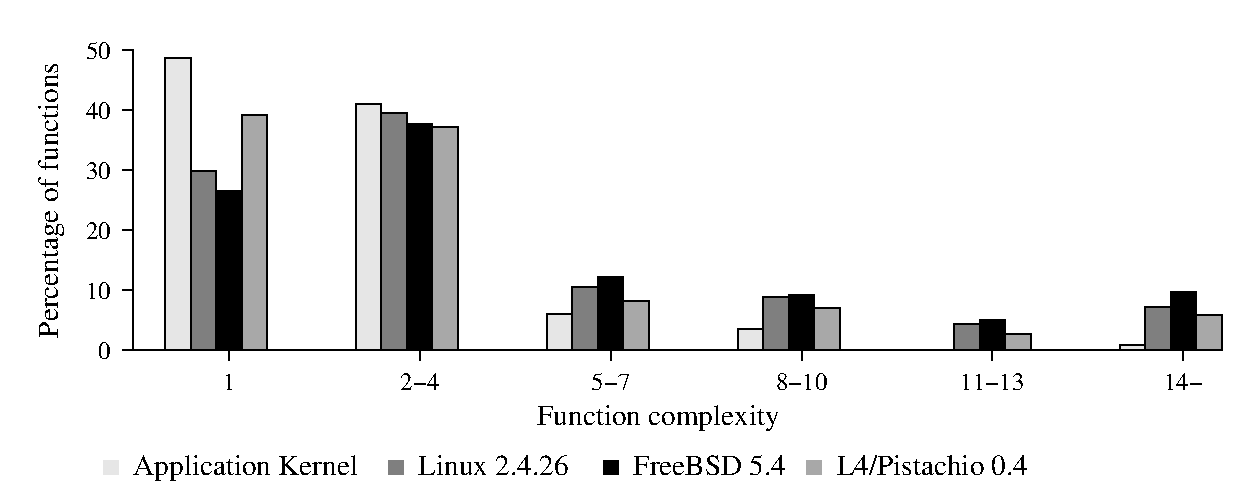
\epsfig{width=1.0\linewidth, file=./data/linux-appkern/mccabe_hist.parsed}
  \caption[Histogram of McCabe cyclomatic complexity]{Histogram of McCabe cyclomatic complexity for the Application
    Kernel, Linux 2.4.26, FreeBSD 5.4 and the L4/Pistachio 0.4 microkernel.}
  \label{fig:mccabe}
\end{figure}

\section{Conclusions and Future Work}
\label{sec:appkern:conclusion}

In this paper we have presented the application kernel, an alternative
approach for adding SMP support to a uniprocessor operating system. Our
approach has lower implementation complexity then traditional approaches,
often without changes to the original uniprocessor kernel, while at the same
time providing scalable performance. In this sense, the application kernel
approach can be seen as a modern revitalization of the master-slave approach.
There are also similarities with approaches used in distributed systems.

We have evaluated a prototype implementation of the application kernel
approach for a uniprocessor Linux kernel, where the results show that our
approach is a viable method to achieve good performance in computationally
intensive applications. We also show that the implementation is quite
straightforward, with a low cyclomatic complexity compared to other operating
system kernels and a small size (around 3,600 lines) requiring only seven
weeks to implement.

There are several advantages with our approach. First, we do not need to
modify the large and complex code of the uniprocessor kernel.  Second, the
development of the uniprocessor kernel can continue as usual with improvements
propagating automatically to the multiprocessor version. Our evaluation also
shows that a large portion of the effort of writing the application kernel can
be reused for other uniprocessor kernels which leads us to believe that our
approach and implementation is fairly generic and reusable for other kernels.

There are a number of optimizations possible for the application kernel
approach. For instance, some threads could run entirely on the bootstrap
kernel, which would mainly be interesting for kernel-bound applications. A
migration scheme similar to that in MOSIX could then be used to
move kernel-bound threads to the bootstrap processor during runtime. Further,
some system calls should be possible to implement directly on the application
kernel, providing the semantics of the system calls are known. For example,
sleeping, yielding the CPU and returning the process ID of the current process
can easily be implemented in the application kernel.

\section*{Acknowledgements}
We would like to thank the anonymous reviewers for their useful feedback. This
work was partly funded by The Knowledge Foundation in Sweden under a research
grant for the project ``Blekinge - Engineering Software Qualities (BESQ)''
(\url{http://www.ipd.bth.se/besq}).

\noindent
The application kernel source code is available as free software licensed
under the GNU GPL at
\url{http://www.ipd.bth.se/ska/application_kernel.html}.


\chapter{Paper~V}
\papertitle{Automatic Low Overhead Program Instrumentation with the LOPI Framework}
  {Simon K�gstr�m, H�kan Grahn, Lars Lundberg}
  {Published in the proceedings of the 9th IEEE Workshop on Interaction
    between Compilers and Computer Architectures, San Francisco, USA, pages
    82--93, February 2005}
\label{cha:paper5}
\label{cha:lopi}
% Add abstract etc?

\section{Introduction}
% This is why we want it.
Program instrumentation is a technique used in many and diverse areas.
Instrumentation is often added to programs in order to investigate performance
aspects of the applications~\cite{paradyn95,etch} as a complement to
statistical profiling such as gprof~\cite{graham83gprof}, Intel
VTune~\cite{wolf99vtune}, or the Digital Continuous Profiling
framework~\cite{anderson97cpw}. Instrumentation is also useful in many
other areas not directly related to performance analysis, for instance call
graph tracing~\cite{steignerwilke2003verstehen}, path
profiling~\cite{ball96efficient}, reversible
debugging~\cite{chen2001reversible}, code coverage analysis, and
security~\cite{miller01pib}.

% They are hard to use
Often, instrumentation is added manually by annotating the source code with
instrumentation points. This task, however, is time-consuming, repetitive and
error-prone, and it is both tied to the high-level language and access to
source code. Over the years, there has therefore been a number of proposals to
alleviate this situation. Today, there exists several libraries, e.g.,
ARM~\cite{armAPI} and PAPI~\cite{london2001papi}, which allows code-reuse for
the instrumentation.  There are also packages that provide graphical
interfaces to select instrumentation-points and several tools for patching
program binaries or relocatable object files~\cite{paradyn95,eel}.

%\emph{What should an instrumentation package fulfil}: Easy to use (no code
%changes, good if application can be patched directly), low overhead, high
%detail, reproducability.
Another problem with program instrumentation is program behavior perturbations
caused by the
instrumentation~\cite{maloney1992instrumentation,moseley2003checking}.
Regardless of how instrumentation is implemented, it always adds extra work
for the program by affecting compiler optimizations (changed register
allocation, reduced inlining possibilities etc.), altering the data reference
patterns, and changing the execution flow.  Taken together, these
perturbations can cause the instrumented program to exhibit a substantially
different behavior than the uninstrumented program.  This problem is
especially severe for performance instrumentation since the instrumented
program should accurately reflect the uninstrumented program, and it is
therefore important to measure and minimize the instrumentation overhead. The
measurement itself can also be a problem, however. Although it is easy to
measure the aggregate overhead of instrumenting a program, observing the
detailed behavior of the instrumentation is harder since any performance
measurement affects the program execution. Taken together, these problems lead
us to we believe that it is important to explore optimizations for
instrumentation, especially for frequently performed operations.
% It is hard to measure instrumentation perturbation

In this paper, we present the LOPI (LOw Perturbation Instrumentation)
framework that provides a generic and easily used framework for instrumenting
programs. In LOPI, we try to optimize for common instrumentation patterns in
order to provide low perturbation on the program behavior. LOPI rewrites
binary ELF-files for GNU/Linux on the IA-32 architecture in order to
instrument an application.  The current implementation instruments function
entry and exit, but the approach is expandable to instrument most points in
the code.

We provide measurements of the instrumentation perturbation using both real
hardware and full-system simulations of seven SPEC CPU2000 benchmarks.  We
compare the LOPI framework to Dyninst\cite{buck00dyninst} and regular
source-based instrumentation.  We find that source-based instrumentation
usually has the lowest instrumentation overhead, on average executing 13\%
more instructions (5\% inlined) for the studied applications, but with more
tedious work for instrumenting the code.  Comparing LOPI and Dyninst we find
that LOPI has lower instruction overhead then Dyninst, on average 36\%
instruction overhead compared to 49\% for Dyninst.  Comparing the total
execution times, we find that source-based instrumentation has 6\% overhead,
LOPI has 22\% overhead, and Dyninst 28\% overhead as compared to an
uninstrumented application.

% In addition, our results show that LOPI generates fewer additional
%cache misses than Dyninst. For example, LOPI generates 57\% more misses in the
%first-level instruction cache, while Dyninst generates 87\% more misses on
%average.

% We have a technique that gives lower instrumentation
% Present some of the main results

The rest of the paper is organized as follows. In Section~\ref{sec:lopi:background}
we provide an overview of program instrumentation, which is followed by an
introduction of the LOPI framework in Section~\ref{sec:lopi:lopi}. In
Section~\ref{sec:lopi:methodology} we present the measurement methodology and in
Section~\ref{sec:lopi:measurements} we provide the measurement results.  Finally,
we discuss related work in Section~\ref{sec:lopi:related_work} and conclude our
findings in Section~\ref{sec:lopi:conclusion}.

\section{Background}
\label{sec:lopi:background}

\subsection{Instrumentation approaches}
Instrumentation packages can be grouped into three broad categories with
different characteristics: \emph{source-based instrumentation}, \emph{binary
  rewriting}, and \emph{memory image rewriting}.  There are some special
cases, for instance instrumentation at the assembly level, but these can
normally be generalized into one of the above (assembly-level instrumentation
is similar to binary rewriting except that it avoids some issues with
relocatable code). Also, some completely different approaches exist.
Valgrind~\cite{valgrind}, for instance, allows instrumentation of unmodified
programs. Valgrind works by running programs in a virtual machine, translating
IA-32 binary code to a intermediate language, applying instrumentation, and
then translated back to IA-32 code again. Valgrind allows instrumenting
unmodified programs, but also imposes a high runtime overhead due to the code
translation. Another approach is to run the application in a simulator, which
gives no perturbation to the actual application, but has issues with accuracy
and speed. Next, we will briefly describe the different approaches.

\begin{enumerate}
\item \textbf{Source-based instrumentation}: Source-based instrumentation
  works by inserting instrumentation calls as statements in the application
  source code. This allows the compiler to optimize the instrumented code, but
  it also inherently produces a different behavior compared to the
  non-instrumented code because of disturbed register allocation, inlining,
  etc. Further, this approach is dependent on the high-level implementation
  language as well as direct access to the source code.

  This category encompasses both libraries for instrumentation, i.e., where
  instrumentation is inserted manually into the source
  code~\cite{london2001papi}, mixed solutions~\cite{garcia2003PET}, and tools
  with source-to-source conversion from a graphical
  interface~\cite{steigner2001cosmos}.

\item \textbf{Binary rewriting}: By patching the executable or the relocatable
  files, the high-level source code of the application can remain untouched.
  This prevents the compiler from optimizing the instrumentation code in the
  context of the application source code, but this should also give a closer
  correspondence to the uninstrumented application. This approach is also
  independent of the high-level language of the application and can in
  principle be used on applications for which the source code is unavailable.

  Many instrumentation packages work this way, for instance ATOM~\cite{atom}
  and EEL~\cite{eel} for UNIX-based systems, Etch~\cite{etch} and
  PatchWrx~\cite{casmira98tcw} for Windows NT systems, and the LOPI
  framework presented here.

\item \textbf{Memory image rewriting} A final approach is to patch the
  application in-core, i.e., after the program has been loaded into memory.
  This approach, used by Dyninst~\cite{buck00dyninst, paradyn95}, allows
  instrumentation to be added to and removed from the program during runtime.
  The characteristics is similar to binary rewriting but memory image
  rewriting allows instrumentation to be dynamically removed when it is no
  longer needed, which can reduce unnecessary overhead.

  Memory image rewriting also adds some other interesting possibilities. Some
  programs, for instance operating system kernels cannot readily be restarted
  in order to have the instrumentation take effect. For these cases, memory
  image rewriting provides the only realistic alternative, and it has also
  been used for instrumentation of the Solaris~\cite{tamches1999kerninst} and
  Linux~\cite{pearce02gdi} kernels.
\end{enumerate}

Each of these methods will cause perturbation to the application. Next we
present an introduction to the various types of perturbation caused by
instrumentation.

\begin{figure*}[t]
  \begin{center}
    \epsfig{width=1.0\linewidth, file=figures/lopi/lopi_overview}
  \end{center}
  \caption[The instrumentation process]{Overview of the instrumentation
    process. The functions and the files to instrument are given on the
    command line.}
  \label{fig:lopi:lipo_overview}
\end{figure*}

\subsection{Instrumentation perturbation}
Instrumentation perturbation is heavily dependent on the type of
instrumentation applied. For performance instrumentation, the instrumentation
might read a set of of hardware performance counters whereas call graph
tracing requires significantly more complex
operations~\cite{steignerwilke2003verstehen}. Some parts are very common
however. At the very basic end, instrumentation always causes more
instructions to be executed, accesses more data in the memory, and can also
cause register spills. Further, there might be kernel invocations, device
access or inter-process communication. The perturbation also varies over
different phases of the program execution:

\begin{itemize}
\item \textbf{Initialization}: Most instrumentation packages have some sort of
  initialization phase. This can include, e.g., the initialization of hardware
  performance counters, creation of data structures, or memory image patching.
  This part can sometimes be very expensive, but is a one-time event.
\item \textbf{Startup-phase}: During the first invocations of the instrumented
  code, the system will run with cold caches and need to bring the code and
  data into the caches.
\item \textbf{Execution}: During the execution of the program, the
  instrumentation adds latency because more instructions are executed,
  increased cache pressure, and (potentially) extra kernel invocations.
\item \textbf{End}: When the program ends, or the instrumentation is removed,
  the instrumentation package usually performs some cleanup operations (for
  instance freeing allocated memory, storing collected data on disk etc.).
  Like the initialization-phase, this is potentially expensive but normally
  has small effects on long-running programs.
\end{itemize}

For the execution phase, there are also some indirect effects on the execution
that can arise from instrumentation. For instance, the addresses of data or
executed instructions might change as a side-effect of instrumentation (this
is especially likely with source instrumentation). The changed addresses can
cause data or code to be aligned differently with respect to cache-lines, and
also in some cases (albeit unusual) change actual program
behavior~\cite{moseley2003checking}. In the LOPI framework, we have tried to
minimize these effects by a number of optimizations, which are described in the
next section.

\section{The LOPI instrumentation framework}
\label{sec:lopi:lopi}
We have implemented an instrumentation package that tries to provide low and
predictable overhead and still provide an easy interface to users.  The
framework uses the binary rewriting approach, although the ideas are
applicable to memory rewriting (such as used by Dyninst) as well. Although we
currently focus on function entry and exit, the approach is possible to
combine with current methods for instrumentation at arbitrary points (still
keeping the optimized entry/exit techniques). We have developed two types of
performance instrumentations for LOPI, one utilizing the PAPI cross-platform
front-end to performance counters~\cite{london2001papi} and one simple
implementation measuring the processor cycle counter with the \texttt{rdtsc}
instruction.

% FIXME: Add some comments on multithreading here

The process of instrumenting a program with the LOPI framework is shown in
Figure~\ref{fig:lopi:lipo_overview}. Using the LOPI framework adds one step in the
compile process - running the LOPI executable after the relocatable files have
been produced. The relocatable ELF-files are then linked with a library
produced by LOPI at runtime, which contains stubs and the user-implemented
instrumentation. Note that selecting the instrumentation points is done
outside the LOPI framework in order to keep the framework general enough to
support different kinds of instrumentation.

\begin{figure*}[htb]
  \begin{center}
    \epsfig{width=1.0\linewidth, file=figures/lopi/non_inst_call}
  \end{center}
  \caption{A non-instrumented function call.}
  \label{fig:lopi:non_inst_call}
\end{figure*}

\begin{figure*}[htb]
  \begin{center}
    \epsfig{width=1.0\linewidth, file=figures/lopi/instrumented_call}
  \end{center}
  \caption[An instrumented function call]{A function call
    instrumented with our approach.}
  \label{fig:lopi:instrumented_call}
\end{figure*}

\begin{figure*}[htb]
  \begin{center}
    \epsfig{width=1.0\linewidth, file=figures/lopi/instrumented_return}
  \end{center}
  \caption[An instrumented function return]{An instrumented function return.}
  \label{fig:lopi:instrumented_return}
\end{figure*}

Before going into details of the operation, we will first briefly
describe the (GCC) calling convention for the IA-32 architecture.
Figure~\ref{fig:lopi:non_inst_call} shows how \emph{caller} calls the
non-instrumented function \emph{callee}.  On IA-32, the
\texttt{call}-instruction pushes the return address to the stack before
switching to the function. On returning with \texttt{ret}, the instruction
pointer is popped from the top of the stack. The IA-32 calling convention
specifies that registers \texttt{\%ebx}, \texttt{\%edi}, \texttt{\%esi}, and
\texttt{\%ebp} are callee-saved, whereas \texttt{\%eax}, \texttt{\%ecx} and
\texttt{\%edx} are caller-saved. Parameters are passed on the stack and the
return value is passed in the \texttt{\%eax} register. The function prologue
shown initializes the function stack frame.

A function entry instrumented with the LOPI framework is shown, somewhat
simplified, in Figure~\ref{fig:lopi:instrumented_call}. When the program execution
reaches an instrumentation point, our library performs a four step operation.
The sequence of events is shown in the figure and described below.

\begin{enumerate}
\item \texttt{enter\_stub} is called (from \emph{callee}) by the overwritten
  function prologue (which was replaced by the instrumentation). The
  \texttt{call}-instruction is immediately followed by an identifier for the
  function (\texttt{func\_nr}). The function identifier defaults to a 8-bit
  value, but if more than 256 functions are instrumented this can be extended
  to a 16- or 32-bit value at instrumentation time (this has not yet been
  implemented, but the extension is simple to make).

\item \texttt{enter\_stub} (shown in Figure~\ref{fig:lopi:instrumented_call}) reads
  the function identifier (which is located at the return address, i.e., in the
  \emph{callee}-prologue). Then, the enter stub calls
  \texttt{instr\_func\_enter}, which is common for all instrumented function
  entries.

\begin{figure}[htb]
  \begin{center}
    \begin{pseudocode}
         \STRUCT{ret\_frame\_t}
          func\_t~~*p\_func \\
          long~~~~~ret\_addr \\
          \COMMENT{For icache/dcache conflict reduction}
          uint8\_t~~padding0[XX] \\
          uint8\_t~~program[16]\\
          uint8\_t~~padding1[XX] \\
          ...
        \ENDSTRUCT
        \\
        ret\_frame\_t ret\_frames[]
        \\
        \\
        \FUNC{instr\_func\_enter}{func\_nr, ret\_addr}
          \COMMENT{Setup return frame}
          ret\_frame = pop\_ret\_frame()\\
          ret\_frame.func = funcs[func\_nr]\\
          ret\_frame.ret\_addr = ret\_addr\\
          *ret\_addr = ret\_frame.program\\
          \\
          \COMMENT{Perform the instrumentation}
          do\_enter\_func(func)
        \ENDFUNC
      \end{pseudocode}
    \end{center}
    \caption{Pseudo code for the \texttt{instr\_func\_enter}-function.}
    \label{fig:lopi:instr_func_entry_code}
\end{figure}

\item The \texttt{instr\_func\_enter}-function, implemented in C (pseudo code
  in Figure~\ref{fig:lopi:instr_func_entry_code}), sets up a return frame to
  instrument the function return. \texttt{inst\_func\_enter} thereafter
  performs the actual instrumentation operation for function entries, which is
  implemented by the user of the instrumentation library and can be inlined.
  Access to the return frames is protected by a spinlock for multithreaded
  programs on SMPs.

\item After returning to the enter stub, the overwritten instructions of the
  function prologue are executed and the control returns to the function
  prologue (after the overwritten instructions).
\end{enumerate}

There are some special cases for instrumenting function entry points, which
suggest separate handling. First, we detect the common function prologue where
the frame pointer (the \texttt{\%ebp} register) is stored and a new stack
frame is setup. This code sequence only varies with a constant, which gives
the size of the new stack frame, and can therefore easily be represented by a
common stub.

\begin{pseudocode}
  pushl~\%ebp~~~~~~~\COMMENT{Save the old frame pointer}
  movl~~\%esp,~\%ebp~\COMMENT{Set the start of the new frame}
  subl~~~\$XX,~\%esp~\COMMENT{Allocate stack space}
\end{pseudocode}

In the seven SPEC CPU2000 benchmarks we used (see
Section~\ref{sec:lopi:methodology}), almost 80\% of the function prologues had this
pattern. This function prologue is represented with a special stub that stores
the stack size \texttt{XX}.  In the rare case that the function prologue is
smaller than 6 bytes (the size of the call-instruction plus the function
identifier) and the first basic block at the same time contains a branch
target within the first 6 bytes, patching the function prologue is unsafe
because the target instruction is overwritten.  LOPI will detect and mark such
areas as unavailable for instrumentation, although this functionality is only
sketched in the prototype implementation.

Function returns are instrumented lazily with the return frames set up in
\texttt{instr\_func\_enter}, i.e., without patching or adding source lines to
the program. The return frame is a data structure with the original return
address (i.e., back to \emph{caller} in this case), which also contains a
machine code stub, copied to the structure at startup. The padding is needed
since the return frame is accessed both as data and executed as code. Without
the padding, the cache block (the stub is only 16 bytes) would ping-pong
between the data and the instruction cache, degrading performance.
The machine code stub acts as a trampoline for the function return
instrumentation. The logic is as follows (refer to
Figure~\ref{fig:lopi:instrumented_return}):

\begin{enumerate}
\item The \emph{callee} function returns with the \texttt{ret} instruction
  (i.e., exactly as without instrumentation). Since the return address was
  overwritten it will return to the return frame stub setup in
  \texttt{instr\_func\_enter}.

\item The return frame stub calls \texttt{instr\_func\_leave}. Since the
  position of the return frame (and thus the return stub) is unknown at
  compile-time, we need to do a register-relative call to
  \texttt{instr\_func\_leave} (not shown in the figure).

\item \texttt{instr\_func\_leave} performs the instrumentation on function
  exit (again specified by the user of the library), deallocates the return
  frame, and returns the original return address (i.e., to \emph{caller} in
  this example). The pseudo code is shown in
  Figure~\ref{fig:lopi:instr_func_leave_code}.
\end{enumerate}

For functions which modify the return address themselves, this optimization is
unsafe, and a revert to a more traditional return instrumentation is needed.
We reduce the perturbation of the instrumented application in a number of ways
both during the program patching and during runtime:

\begin{figure}
  \begin{center}
    \begin{pseudocode}
      \FUNC{instr\_func\_leave}{}
        \COMMENT{This code is contained in the ret\_frame}
        ret\_frame = [return address]-XX \\
        \COMMENT{Perform the instrumentation}
        do\_leave\_func(ret\_frame.func) \\
        \\
        push\_ret\_frame(ret\_frame) \\
        \COMMENT{Found in the ret\_frame}
        \RETURN{[original return address]}
      \ENDFUNC
    \end{pseudocode}
  \end{center}
  \caption{Pseudo code for the \texttt{instr\_func\_leave}-function.}
  \label{fig:lopi:instr_func_leave_code}
\end{figure}

\begin{table*}[thb]
  \begin{center}
    \caption[Benchmark description]{Description of the SPEC CPU2000 benchmarks
      used in this study.}
  \label{tab:lopi:benchmarks}
  \begin{tabular}{|l|l|l|}
       \hline
       \hline
       Benchmark  & Description & Data set size \\
       \hline
       \hline
       164.gzip   & Compression & lgred.log \\
       \hline
       176.gcc    & Compiler & smred.c-iterate.i \\
       \hline
       181.mcf    & Combinatorial optimization & lgred.in \\
       \hline
       183.equake & Simulation of seismic wave propagation & lgred.in \\
       \hline
       197.parser & Grammar analysis & lgred.in \\
       \hline
       256.bzip2   & Compression & lgred.graphic \\
       \hline
       300.twolf   & CAD, Placement and global routing & lgred \\
       \hline
       \hline
  \end{tabular}
  \end{center}
\end{table*}

\begin{enumerate}
\item \textbf{Inlined function identifiers}. The function identifier (shown in
  Figure~\ref{fig:lopi:instrumented_call}) is placed directly in the instrumented
  code in order to avoid the need for calling separate stubs for every
  instrumentation point. The function identifier also allows us to lookup
  meta data for the instrumentation point by using it as a vector index
  instead of performing an expensive hash table lookup.
\item \textbf{Code reuse}. A call-stub is shared for every instrumentation
  point with the same overwritten instructions. Also, the stubs are kept as
  short of possible with most of the logic in the generic enter and exit
  functions.
\item \textbf{Optimize for common cases}. We use a special stub for the common
  stack frame setup as explained in Section~\ref{sec:lopi:lopi}. This helps down the
  i-cache miss rate by reducing the number of instrumentation stubs.

\item \textbf{Register saving}. Our entry stubs does not store any registers
  for the function entries since we do not use any callee-saved registers in
  the stub. The return frame saves the \texttt{\%eax} register since this is
  used for return values on IA-32.
\item \textbf{Data reuse}. The return frames are allocated in a stack-based scheme
  where the most recently used return frame is reused first.
\end{enumerate}

The pollution of the instruction cache is limited by the number of function
call stubs used in the instrumentation and the number of return frames used.
The number of active return frames at a given point of time is equal to the
current nesting depth of the instrumented functions, in most cases a fairly
low number (the worst case occurs with deep recursion).

Taken together, these optimizations significantly reduce the overhead
of instrumentation. Further, since the call-stubs are aggressively reused, we
expect the perturbation to be more predictable since less code is added to the
program. The next section presents measurements comparing our approach to the
Dyninst tool and basic source-based instrumentation.

\section{Measurement methodology}
\label{sec:lopi:methodology}
% Why simics?
For our measurements, we have used both real hardware and the Simics
full-system simulator~\cite{simics}.  The machine we used is a Pentium III
system running Linux, with a 1~GHz processor and 256 MB RAM. We use
the hardware performance counters available on the Pentium III (through the
PAPI~\cite{london2001papi} library) to capture the measures presented in
Table~\ref{tab:lopi:agg_overhead}, e.g., the number of instructions and cache
misses.

\begin{figure*}[htb]
  \begin{center}
    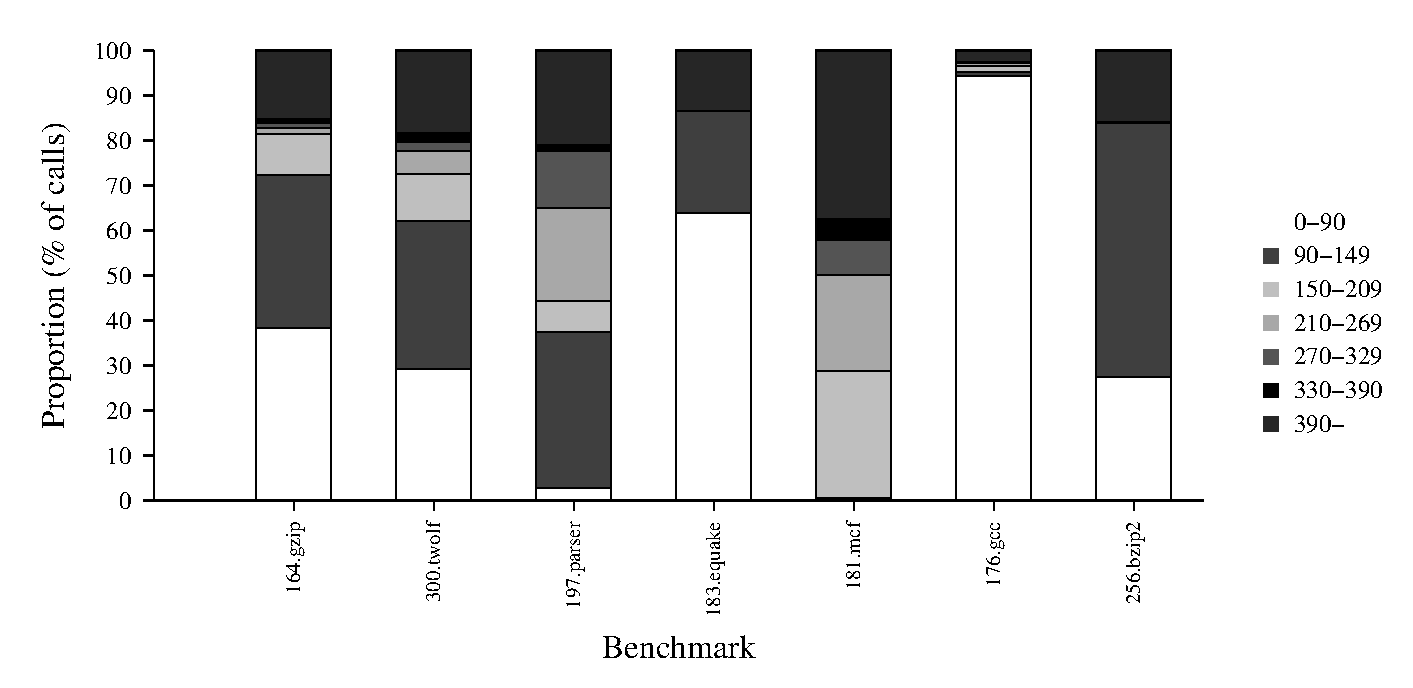
\epsfig{width=1.07\linewidth, file=data/lopi/eps/1_func_avgs_STACKED_reduced}
  \end{center}
  \caption[Cycles per function call]{Cycles per function call on a subset of
    the SPEC CPU2000 benchmarks.}
  \label{fig:lopi:function_averages}
\end{figure*}

As for our simulations, we simulate a complete Pentium III system with caches
running a real operating system for performing the instrumentation
measurements. The simulated system has 16 KB, 4-way set-associative,
first-level data and instruction caches, and a unified 512KB, 8-way
set-associative, second-level cache. Simics allows us to create a complete
non-intrusive measurement of the application execution, both for instrumented
and non-instrumented applications. We can therefore isolate the impact of
instrumentation from the application traces. We use Simics to provide detailed
execution characteristics which were not possible to capture on real hardware,
i.e., the figures in Figure~\ref{fig:lopi:exec_profile}.

%A drawback with using
%Simics is that (at the time of our measurements) it did not provide exact
%instruction timing on IA-32, which means that the cycle count will differ from
%measurements on real hardware.

% How is the simulated tracing done
% 80%..
We ran tests with seven applications from the SPEC CPU2000 benchmarks
(compiled with GCC 2.95.4, optimization level -O3) on a minimal Linux
2.4.22-based system.  A short description of the selected benchmarks is
presented in Table~\ref{tab:lopi:benchmarks}.  All measurements ran with the
MinneSPEC~\cite{minnespec} workloads in order to provide reasonable execution
times in the simulated environment and each of the tests ran to completion.
We chose to instrument the functions that make up 80\% of the total execution
time (as reported by gprof). Unfortunately, with Dyninst we were unable to
instrument three of the applications when running on real hardware due to a
software upgrade.

The simulator was setup to flush the caches when starting the program (i.e.,
at ``main'', after the instrumentation package setup) to avoid situations
where data was brought into the caches before the program execution starts
(for instance because of the instrumentation package startup-phase touching
the functions).  Our accumulated values for real hardware excludes
initialization and cleanup of the instrumentation library, but does not
invalidate the cache contents.

The benchmarks were instrumented with four methods, source-based
instrumentation (split in inlined and non-inlined operation), Dyninst (version
4.0.1 of the Dyninst API, function instrumentation with tracetool), and our
LOPI framework. The source-based instrumentation was added by hand, a tedious
task that required us to add instrumentation points to over 500 places for
the largest benchmark (176.gcc). The 176.gcc benchmark also illustrates the
effectiveness of our stub reuse, requiring only two stubs for 54 instrumented
functions. For all 92 instrumentation points (in all benchmarks), totally 5
different stubs were needed.

% User-level code (np, we dont access the kernel)
To get comparable results, we implemented the same instrumentation for each
package. The instrumentation performs a fairly common instrumentation
operation, reading a 4-byte value at function entry and accumulating it at the
function exit, similar for instance to accumulating a hardware performance
counter (the kernel is not accessed). We exclude the perturbation caused by
the OS kernel in our simulated environment by pausing the measurements on
kernel entry and starting them again on kernel entry (the simulated caches are
also disabled when executed kernel code). This was done to avoid timing
behavior to affect the measurements and also to make the measurements more
OS-independent.


\begin{table*}[t!]
  \begin{center}
  \normalsize
  \caption[SPEC benchmark overhead.]{\emph{Continued on next page.}}
  \vspace{0.2in}
  \label{tab:lopi:agg_overhead}
  \scriptsize
  \begin{tabular}{ll|r|r|rr}
    \cline{3-6}
    && Cycles & Instructions & \multicolumn{2}{|c|}{Branches} \\
    \cline{3-6}
    \multicolumn{2}{l}{Benchmark} &  & &  nr  & miss pred. \\
    \hline
    \hline
    %                Cycl    Insns  Bnr    BmP  
164.gzip & src  & 1.03 & 1.06 & 1.06 & 1.00 \\
 & src (inline) & 1.01 & 1.02 & 1.02 & 1.03 \\
 & LOPI         & 1.17 & 1.16 & 1.13 & 1.74 \\
 & Dyninst      & 1.25 & 1.21 & 1.23 & 1.00 \\
\hline
176.gcc
 & src          & 1.09 & 1.13 & 1.11 & 1.07 \\
 & src (inline) & 1.02 & 1.05 & 1.03 & 0.99 \\
 & LOPI         & 1.37 & 1.42 & 1.30 & 1.51 \\
 & Dyninst      &  n/a &  n/a &  n/a &  n/a \\
\hline
181.mcf
 & src          & 1.17 & 1.46 & 1.38 & 1.00 \\
 & src (inline) & 1.04 & 1.18 & 1.13 & 0.90 \\
 & LOPI         & 1.43 & 2.17 & 1.88 & 2.16 \\
 & Dyninst      & 1.67 & 2.50 & 2.51 & 1.02 \\
\hline
183.equake
 & src          & 1.00 & 1.00 & 1.01 & 1.00 \\
 & src (inline) & 1.00 & 1.00 & 1.00 & 0.99 \\
 & LOPI         & 1.01 & 1.02 & 1.02 & 1.03 \\
 & Dyninst      & 1.01 & 1.02 & 1.03 & 1.00 \\
\hline
197.parser
 & src          & 1.03 & 1.07 & 1.06 & 1.02 \\
 & src (inline) & 1.01 & 1.03 & 1.02 & 1.01 \\
 & LOPI         & 1.11 & 1.19 & 1.15 & 1.36 \\
 & Dyninst      & 1.21 & 1.24 & 1.25 & 1.03 \\
\hline
256.bzip2
 & src          & 1.04 & 1.08 & 1.11 & 0.99 \\
 & src (inline) & 1.02 & 1.04 & 1.04 & 1.00 \\
 & LOPI         & 1.21 & 1.22 & 1.26 & 2.47 \\
 & Dyninst      &  n/a &  n/a &  n/a &  n/a \\
\hline
300.twolf
 & src          & 1.08 & 1.12 & 1.15 & 1.03 \\
 & src (inline) & 1.01 & 1.05 & 1.04 & 1.01 \\
 & LOPI         & 1.25 & 1.33 & 1.33 & 1.34 \\
 & Dyninst      &  n/a &  n/a &  n/a &  n/a \\
\hline
\hline
Average
 & src          & 1.06 & 1.13 & 1.13 & 1.01 \\
 & src (inline) & 1.02 & 1.05 & 1.04 & 0.99 \\
 & LOPI         & 1.22 & 1.36 & 1.30 & 1.66 \\
 & Dyninst      & 1.28 & 1.49 & 1.50 & 1.01 \\

    \hline
    \hline
  \end{tabular}
  \end{center}
\end{table*}

\begin{table*}[t!]
  \begin{center}
  \begin{flushleft}
    Table~\ref{tab:lopi:agg_overhead}: Aggregate overhead for the SPEC
    benchmarks. Dyninst average values are caclulated from the successful
    benchmarks.
  \end{flushleft}
  \vspace{0.2in}
  \scriptsize
  \begin{tabular}{ll|rr|rr|rr}
    \cline{3-8}
    && \multicolumn{2}{|c|}{L1 Dcache}&\multicolumn{2}{|c|}{L1 Icache}&\multicolumn{2}{|c|}{L2 unified}\\
    \cline{3-8}
    \multicolumn{2}{l}{Benchmark} & refs & misses & refs & misses & refs & misses \\
    \hline
    \hline
    %                L1Dr   L1Dm   L1Ir   L1Im   L2Ur   L2Um
164.gzip & src  & 1.10 & 1.01 & 1.02 & 1.02 & 1.01 & 1.02 \\
 & src (inline) & 1.04 & 1.01 & 0.97 & 0.95 & 1.01 & 0.97 \\
 & LOPI         & 1.29 & 1.04 & 1.12 & 1.06 & 1.03 & 1.20 \\
 & Dyninst      & 1.43 & 1.02 & 1.23 & 1.14 & 1.02 & 1.16 \\
\hline
176.gcc
 & src          & 1.16 & 1.06 & 1.11 & 1.03 & 1.03 & 0.97 \\
 & src (inline) & 1.06 & 1.05 & 1.02 & 1.05 & 1.05 & 0.96 \\
 & LOPI         & 1.54 & 1.32 & 1.46 & 1.13 & 1.14 & 1.08 \\
 & Dyninst      &  n/a &  n/a &  n/a &  n/a &  n/a &  n/a \\
\hline
181.mcf
 & src          & 1.61 & 0.99 & 1.18 & 1.06 & 0.99 & 0.99 \\
 & src (inline) & 1.23 & 1.00 & 1.04 & 1.02 & 1.00 & 1.01 \\
 & LOPI         & 2.62 & 1.14 & 1.43 & 1.65 & 1.00 & 0.99 \\
 & Dyninst      & 3.39 & 0.99 & 1.69 & 1.24 & 0.99 & 0.98 \\
\hline
183.equake
 & src          & 1.01 & 1.00 & 1.00 & 1.00 & 1.00 & 1.00 \\
 & src (inline) & 1.01 & 1.00 & 1.00 & 1.31 & 1.02 & 1.00 \\
 & LOPI         & 1.02 & 1.04 & 1.02 & 1.04 & 1.04 & 1.01 \\
 & Dyninst      & 1.03 & 1.04 & 1.02 & 1.00 & 1.03 & 1.01 \\
\hline
197.parser
 & src          & 1.08 & 1.00 & 1.03 & 0.97 & 1.00 & 1.00 \\
 & src (inline) & 1.03 & 1.00 & 1.01 & 1.01 & 1.00 & 1.00 \\
 & LOPI         & 1.25 & 1.02 & 1.11 & 1.66 & 1.02 & 1.01 \\
 & Dyninst      & 1.37 & 1.01 & 1.21 & 1.06 & 1.01 & 0.99 \\
\hline
256.bzip2
 & src          & 1.09 & 1.00 & 1.04 & 1.06 & 1.00 & 1.00 \\
 & src (inline) & 1.04 & 1.00 & 1.01 & 1.01 & 1.00 & 1.00 \\
 & LOPI         & 1.28 & 1.00 & 1.20 & 1.15 & 1.00 & 1.00 \\
 & Dyninst      &  n/a &  n/a &  n/a &  n/a &  n/a &  n/a \\
\hline
300.twolf
 & src          & 1.14 & 1.02 & 1.08 & 1.75 & 1.03 & 0.58 \\
 & src (inline) & 1.06 & 1.01 & 1.01 & 1.28 & 1.02 & 0.97 \\
 & LOPI         & 1.39 & 0.95 & 1.25 & 1.28 & 0.96 & 0.75 \\
 & Dyninst      &  n/a &  n/a &  n/a &  n/a &  n/a &  n/a \\
\hline
\hline
Average
 & src          & 1.17 & 1.01 & 1.07 & 1.13 & 1.01 & 0.94 \\
 & src (inline) & 1.07 & 1.01 & 1.01 & 1.09 & 1.01 & 0.99 \\
 & LOPI         & 1.48 & 1.07 & 1.23 & 1.28 & 1.03 & 1.00 \\
 & Dyninst      & 1.80 & 1.01 & 1.29 & 1.11 & 1.01 & 1.03 \\

    \hline
    \hline
  \end{tabular}
  \end{center}
\end{table*}

\section{Measurement results}
\label{sec:lopi:measurements}

Figure~\ref{fig:lopi:function_averages} shows the average number of instructions
per function for a subset of the SPEC CPU2000 benchmarks. The length includes
that of called functions (even for recursive function calls). From the figure,
we can get a feeling for the cost of instrumenting functions, i.e.,
instrumenting a program with frequent short functions is likely to be more
costly than instrumenting one with longer functions. We observe that for many
applications, e.g., 164.gzip, 176.gcc and 300.twolf, a large proportion of the
functions are shorter than 90 instructions (183.equake also show a large
proportion of short instruction, but almost all work is done in a few
long-running functions). This indicates that keeping the cost of instrumenting
a function as low as possible is very important for these programs.

Table~\ref{tab:lopi:agg_overhead} provides aggregate execution times/overhead and
cache behavior with source instrumentation (both inlined and not inlined),
Dyninst, and the LOPI framework. We see that source instrumentation,
particularly inlined, is the approach with lowest overhead (on average 13\%
more instructions non-inlined and 5\% inlined). This is an expected result
since the source instrumentation can be optimized by the compiler. LOPI and
Dyninst execute 36\% and 49\% more instructions, respectively, than an
uninstrumented application. In terms of execution time, we find that LOPI
generates 22\% longer execution times on average and Dynint 28\% longer
execution times than an uninstrumented application.

\begin{figure*}[t!]
  \centering{183.equake}
  $\begin{array}{cc}
    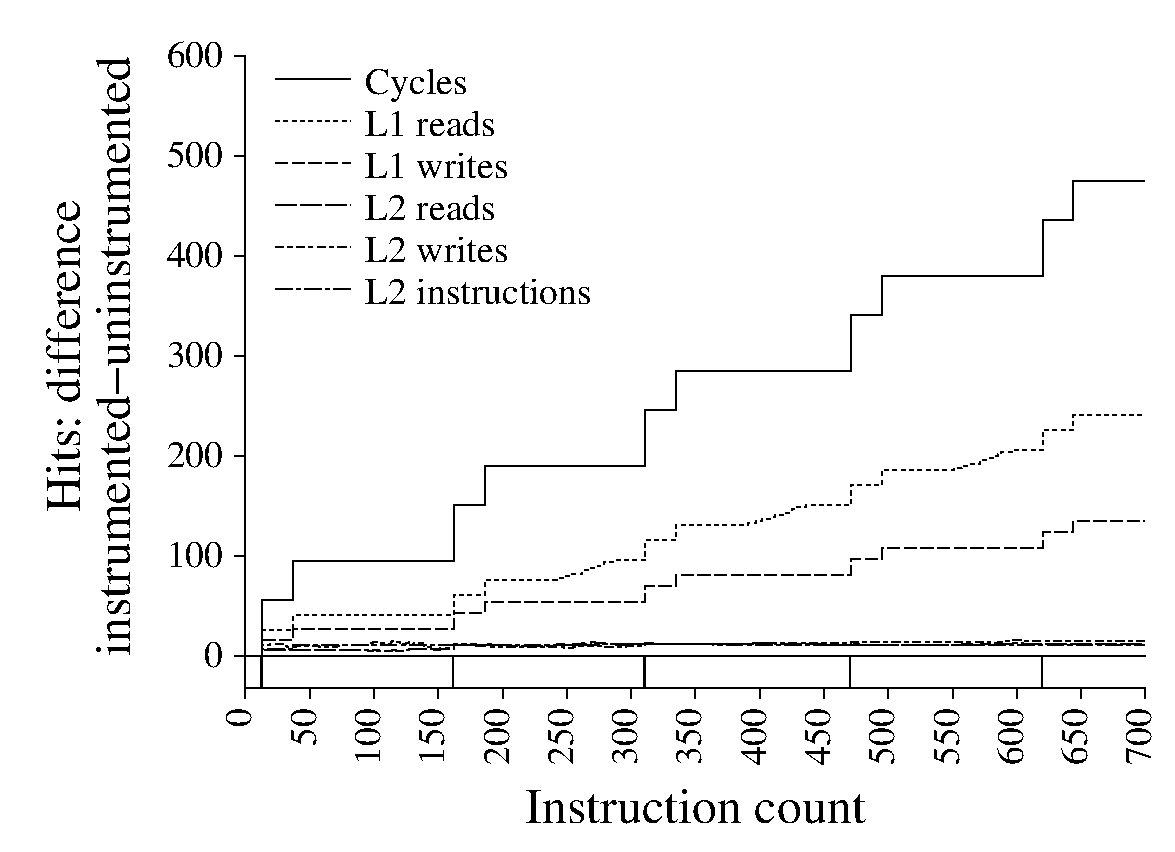
\epsfig{height=0.38\linewidth, file=data/lopi/eps/hits_183.equake_inso_exact} &
    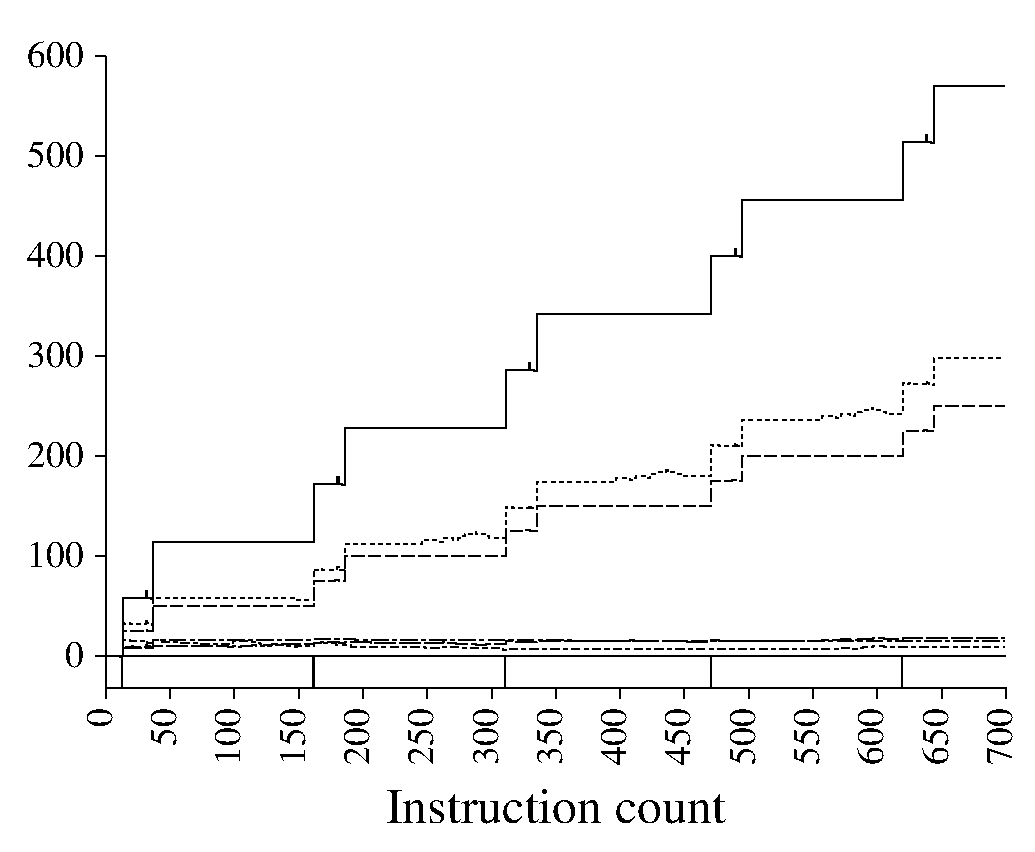
\epsfig{height=0.38\linewidth, file=data/lopi/eps/hits_183.equake_dyninst_exact} \\
    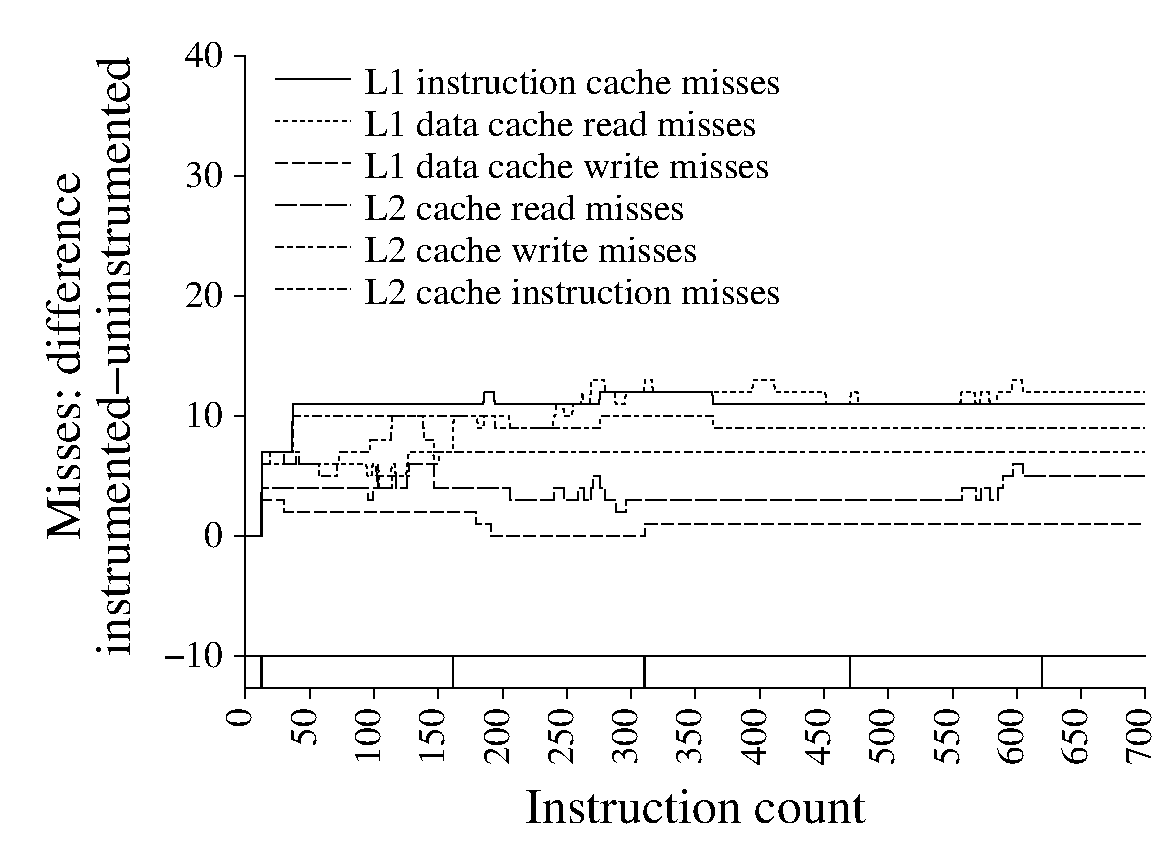
\epsfig{height=0.38\linewidth, file=data/lopi/eps/misses_183.equake_inso_exact} &
    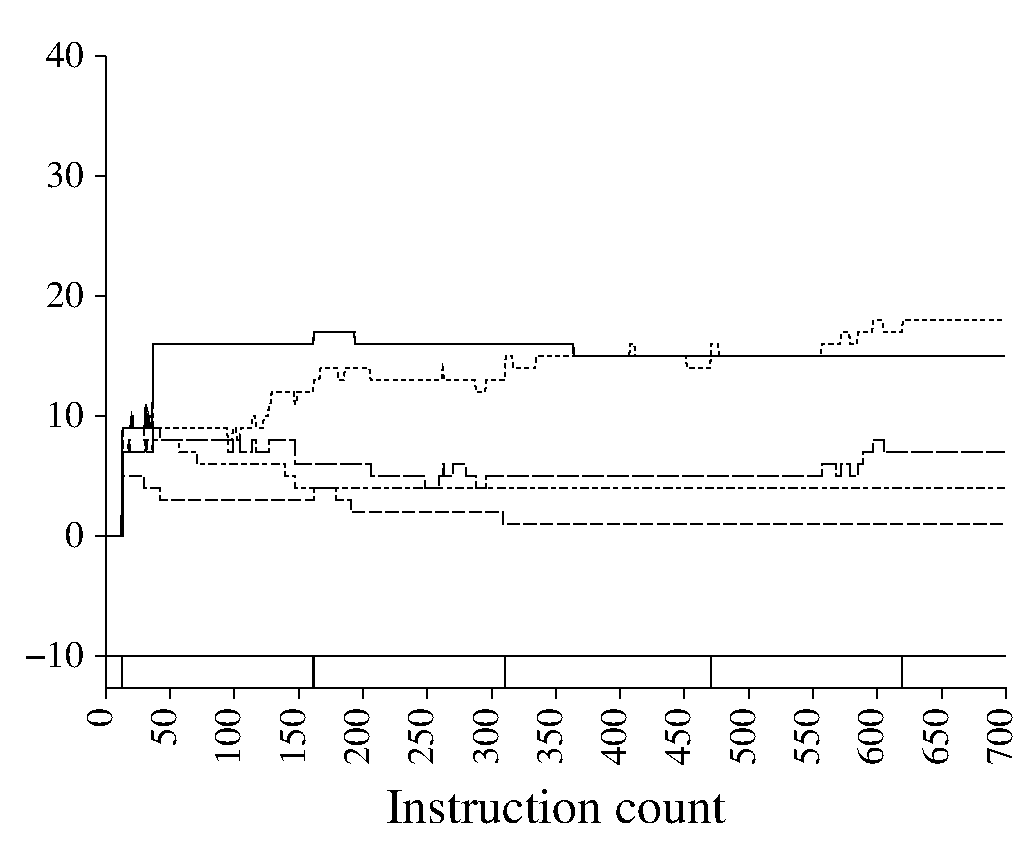
\epsfig{height=0.38\linewidth, file=data/lopi/eps/misses_183.equake_dyninst_exact} \\
  \end{array}$
  \caption[Execution profile for two SPEC benchmarks.]{\emph{Continued on next
    page.}}
  \label{fig:lopi:exec_profile}
\end{figure*}
\begin{figure*}[t!]
  \centering{197.parser}
  $\begin{array}{cc}
    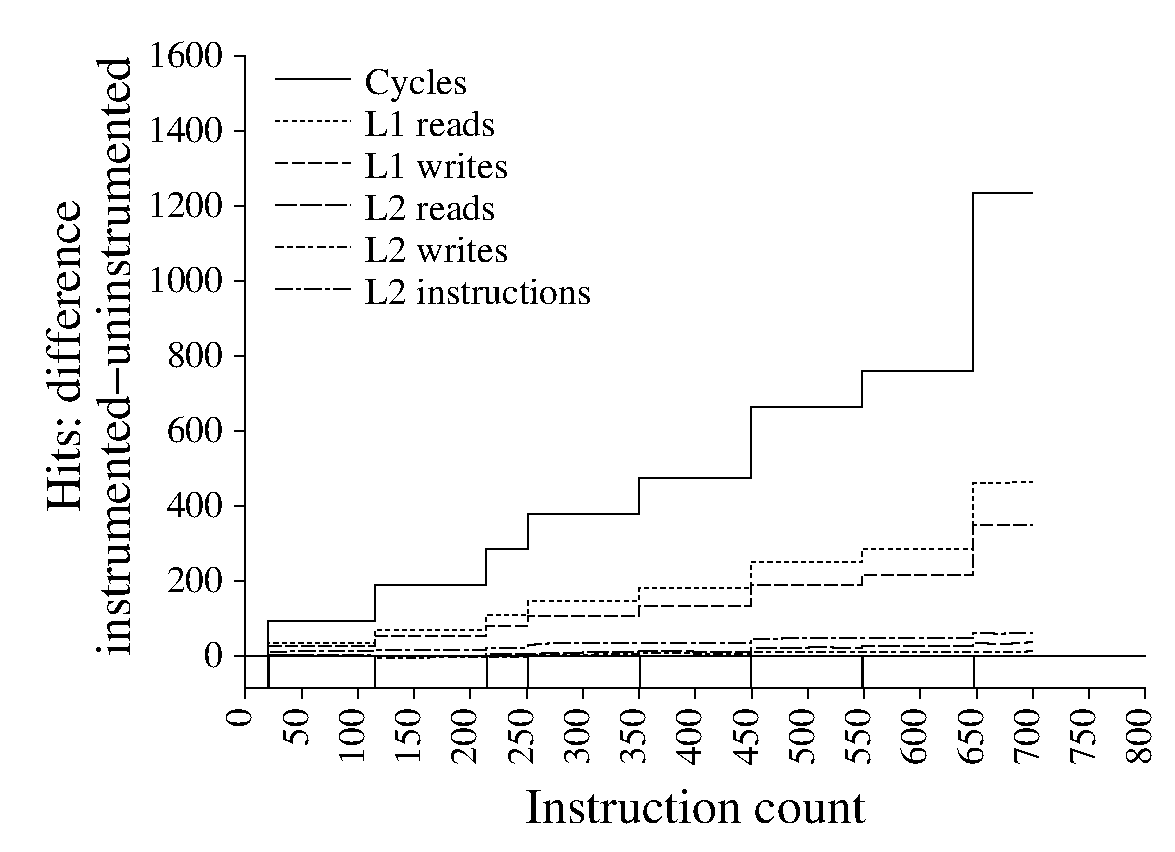
\epsfig{height=0.38\linewidth, file=data/lopi/eps/hits_197.parser_inso_exact} &
    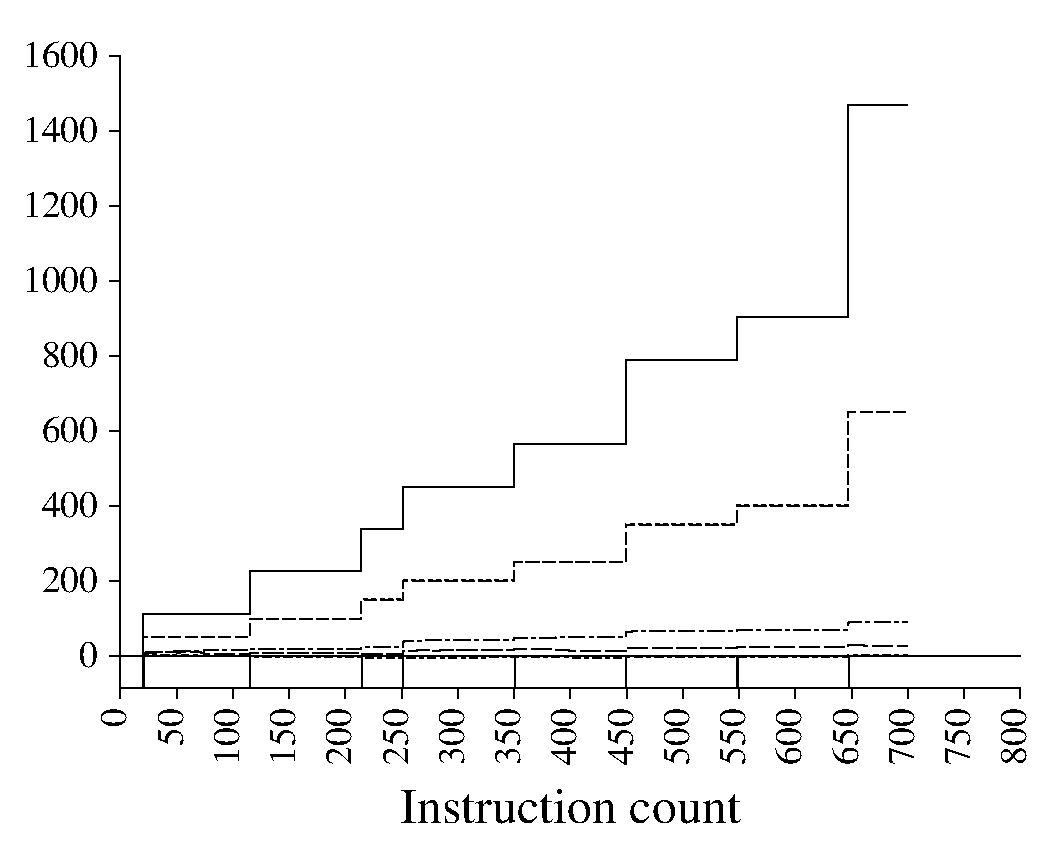
\epsfig{height=0.38\linewidth, file=data/lopi/eps/hits_197.parser_dyninst_exact} \\
    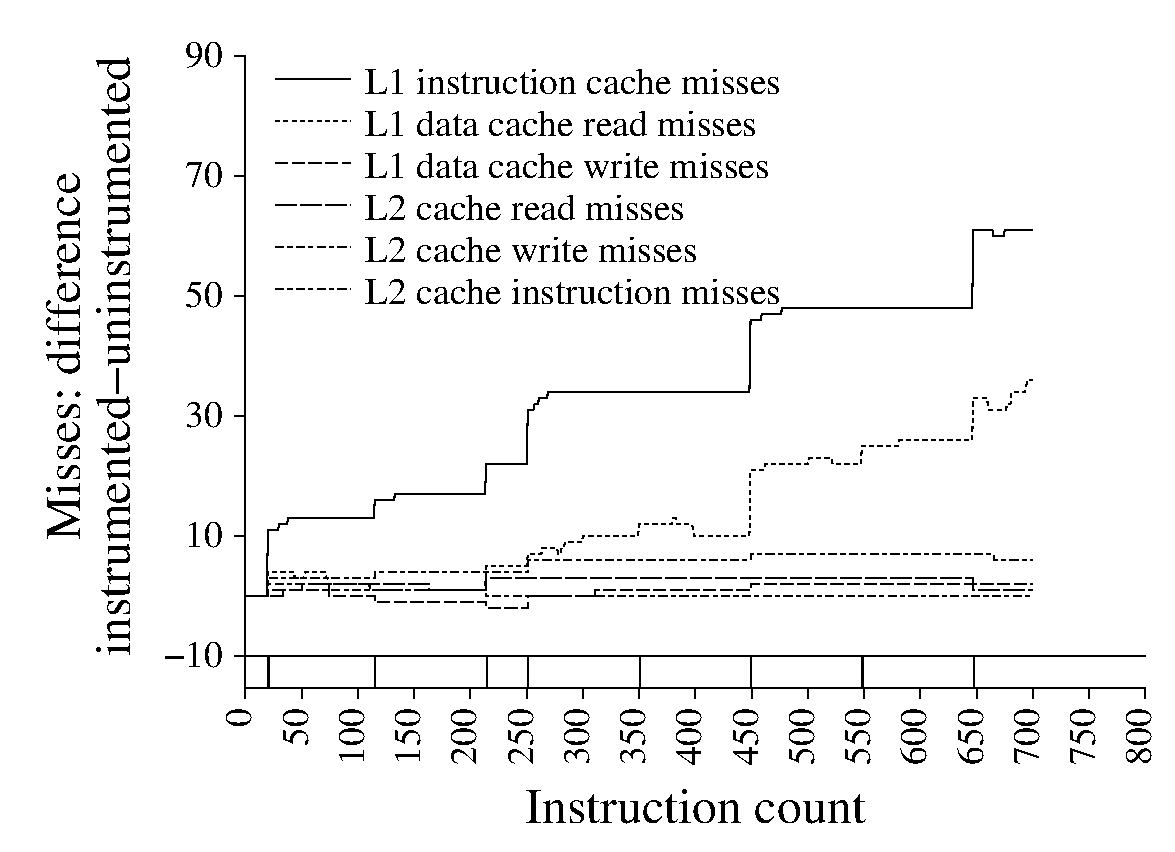
\epsfig{height=0.38\linewidth, file=data/lopi/eps/misses_197.parser_inso_exact} &
    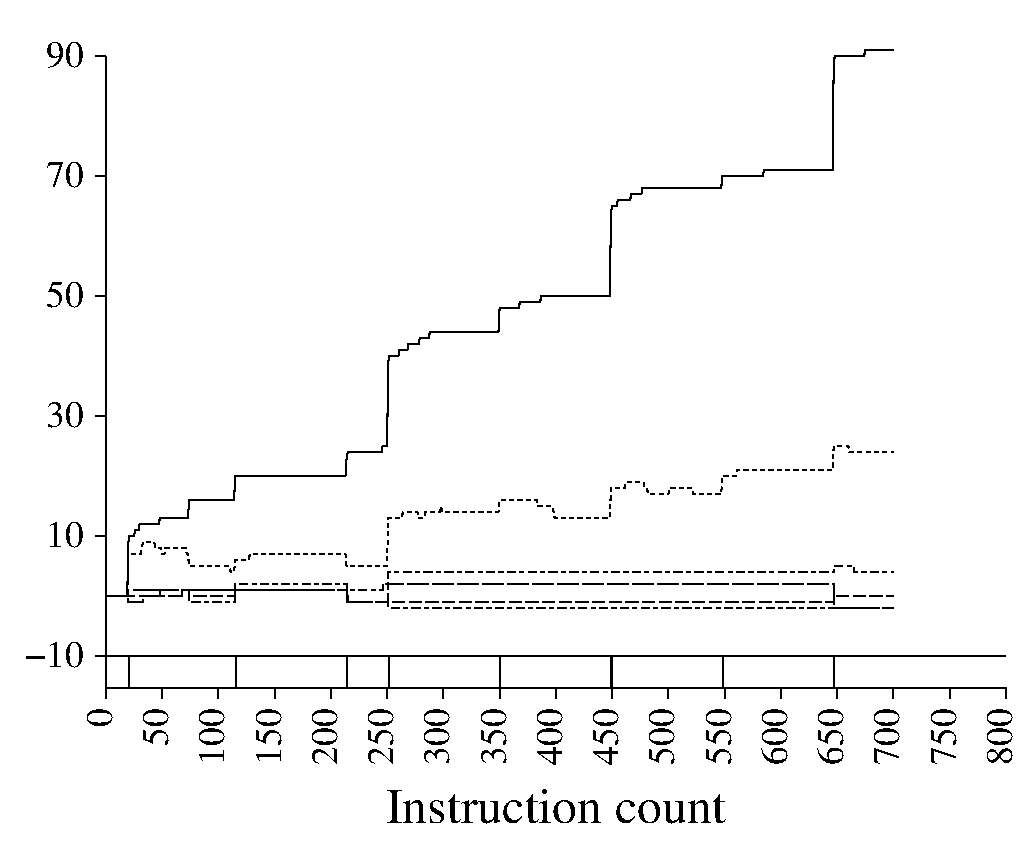
\epsfig{height=0.38\linewidth, file=data/lopi/eps/misses_197.parser_dyninst_exact} \\
  \end{array}$
  \begin{flushleft}
    Figure~\ref{fig:lopi:exec_profile}: Partial execution
    profile for 183.equake and 197.parser. LOPI is shown on the left, Dyninst
    on the right.
  \end{flushleft}
\end{figure*}

Analyzing the cache misses we find that LOPI generates fewer first level cache
accesses on average than Dyninst does, but LOPI has more first-level cache
misses than Dyninst. This indicates a higher locality in the Dyninst code.
However, when we look at the second-level cache accesses we find that the
number of misses is comparable for LOPI and Dyninst.  One reason for the
higher number of data read misses for LOPI is that the return frames (which
are logically code) are allocated as data.

We have identified one performance limitation for LOPI~-- a high number of
miss-predicted branches. The Pentium III employs a branch predictor for
function returns, which work as long as functions are called in the ``normal''~
manner, i.e., through a \texttt{call}/\texttt{ret} pair. Since LOPI overwrites
the return address with an address in the return frame, the return branch
predictor misses its prediction, resulting in a performance loss. This problem
was not visible in the simulated results.

Figure~\ref{fig:lopi:exec_profile} presents a partial execution profile for the
183.equake and 197.parser SPEC benchmarks.  The figure shows the difference
between an instrumented and a non-instrumented run for both LOPI and Dyninst
(note that the graph does not show the absolute values, which start at higher
than zero).  The profiles are constructed from a trace of every instruction in
the shown code snippet (except for the instrumentation code), i.e., every
point in time in the figure corresponds to one instruction in the
non-instrumented code.  Instrumentation points for function entries are shown
as vertical bars below the x-axis.

The 183.equake profile comes from the execution of a nested execution loop,
which calls three short functions \emph{phi0}, \emph{phi1}, and \emph{phi2}
where \emph{phi2} is instrumented. For the 197.parser profile, the
instrumented section shows a section with numerous recursive function calls.
As the Figure shows, the return frames cause some pressure on the caches when
the frames cannot be reused on deeper levels of function nesting (because of
the recursion). This is especially visible for L1 read misses that increase
with each additional instrumented call in Figure~\ref{fig:lopi:exec_profile}.

From the graphs, we can see that the Dyninst instrumentation is more intrusive
than our instrumentation. Our instrumentation is mainly cheaper when
instrumenting the function returns (shown as the second climb in the upper
graphs), which shows that the lazy return instrumentation pays off. We can also
see that the number of cache misses is somewhat higher for Dyninst, although
both instrumentation packages primarily cause cache misses on the first
invocation.
% Comment side effects?


\section{Related work}

\label{sec:lopi:related_work}
In this section we discuss some other tools that are similar to our
instrumentation framework. We start with those that rewrite binary files in
order to instrument an application. Examples of such tools are
PatchWrx~\cite{casmira98tcw}, Etch~\cite{etch}, ATOM~\cite{atom}, and
EEL~\cite{eel}. We thereafter discuss Dyninst~\cite{buck00dyninst, paradyn95},
which rewrites the memory image in order to instrument an application.

PatchWrx, ATOM, and EEL works on RISC processors, where it is easier to
rewrite and patch a binary file since all instructions have the same size. In
order to patch and trace an instruction, you simply replace the traced
instruction with a branch instruction to a code snippet where the replaced
instruction together with the instrumentation code reside. In contrast,
rewriting a binary file for an IA-32-processor is much harder due to variable
instruction length. Etch and LOPI both works for IA-32-binaries, and Dyninst
is available for both RISC and CISC processors.

PatchWrx~\cite{casmira98tcw} is developed for Alpha processors and Windows
NT. PatchWrx utilizes the PALcode on the Alpha processor to capture traces,
and it can patch, i.e., instrument, Windows NT application and system binary
images. PatchWrx replaces all types of branching instructions with
unconditional branches to a patch section where the instrumentation code
reside. PatchWrx can also trace loads and stores by replacing the load or
store instruction with an unconditional branch to the instrumentation code,
where also the replaced load or store resides.

ATOM~\cite{atom} is developed for Alpha processors and works under Tru64 UNIX.
ATOM is a general framework for building a range of program analysis tools,
e.g., block counting, profiling, and cache simulation. ATOM allows a procedure
call to be inserted before and after any procedure, basic block, or
instruction. The user indicates where the instrumentation points are, and
provides analysis routines that are called at the instrumentation points.
ATOM then builds an instrumented version of the application including the
analysis routines.

EEL~\cite{eel} (Executable Editing Library) is a library for building tools to
analyze and modify executable files. It can be used, e.g., for program
profiling and tracing, cache simulation, and program optimization. EEL runs on
SPARC processors under Solaris, and provides a mostly architecture- and
system-independent set of operations to read, analyze and modify code in an
executable file.  The user can provide code snippets that can be inserted at
arbitrary places in the binary code. EEL is capable of sophisticated code
analysis, e.g., control-flow graph analysis and live/dead register analysis.

Etch~\cite{etch} is a general-purpose tool for rewriting Win32 binaries for
IA-32-processors. Etch provides a framework for handling the complexities of
both the Win32 executable format as well as the IA-32 instruction set. Important
issues with the Win32 format that Etch solves are to correctly identify code
and data sections, as well as identification of all dynamically loaded
libraries and modules. Etch can be used, e.g., for tracing all loads and
stores, measuring instruction mixes, and code transformation for performance
improvements.  There is also a graphical user interface provided with Etch.

Dyninst~\cite{buck00dyninst, paradyn95} patches and instruments the application
in-core, i.e., after the program has been loaded into memory.  This approach
allows instrumentation to be added to and removed from the program during
runtime. For example, instrumentation can be added where new hot-spots in the
code are detected during runtime, and instrumentation can be dynamically
removed when it is no longer needed, which can reduce unnecessary overhead.
Memory image rewriting also opens up the possibility to instrument operating
system kernels~\cite{tamches1999kerninst}, which cannot be restarted in order
to have the instrumentation take effect.

Pin~\cite{luk05pin,Pinpoint} is a tool for dynamic instrumentation of Linux
applications available for IA-32e, ARM, Itanium and IA-32e. It provides an API
for inserting function calls to user-defined measurement functions at
arbitrary points in the code. Pin performs the program instrumentation at run
time, using a just-in time compiler to instrument and translate the
application.  As a result, Pin can handle shared libraries, multi-threaded
applications, as well as mixed code and data.
% FIXME: Check similarities between Valgrind and pin

\section{Conclusions}
\label{sec:lopi:conclusion}

Program instrumentation is an important technique in many areas, e.g.,
performance measurements, debugging, and coverage analysis.  To be useful,
instrumentation must be easy to apply and it should perturb the application
execution as little as possible. In this paper we present and evaluate the
LOPI framework, which provides a low-overhead generic solution to program
instrumentation.  The LOPI framework automatically instruments an application
by rewriting the binary file(s) by adding one step in the compilation process.
LOPI gives low overhead by applying techniques to reduce the number of added
instructions to the program and by using a lazy method for instrumenting
function returns.

We provide detailed measurements of the instrumentation perturbation using
hardware and full-system simulations of seven SPEC CPU2000 benchmarks. We
compare the LOPI framework to the state-of-the-art Dyninst package and regular
source-based instrumentation.  The measurements show that source-based
instrumentation has the lowest instruction overhead, on average 13\%, but
requires significantly more tedious work for instrumenting the code.
Comparing LOPI and Dyninst we find that LOPI has lower instruction overhead
than Dyninst, on average 36\% as compared to 49\%, respectively. In terms of
execution time, LOPI increases the execution time by 22\% compared to
uninstrumented operation whereas Dyninst adds 28\%.

% FIXME: Add discussion about code splicing here
We believe that the LOPI framework is a viable and flexible way for automatic
program instrumentation with low perturbation. Future work on LOPI involves
adding support for instrumentation at arbitrary program locations, which would
require copying overwritten instruction into the entry stub and saving live
registers at the instrumentation point. Like Dyninst does, this would require
careful handling of replacing instructions, especially on architectures with
variable-length instructions. Another possibility is to port the framework to
other architectures than IA-32, which could require other optimizations than
those explored here.

\section*{Availability}
\noindent
LOPI is available as free software licensed under the GNU GPL at
\url{http://www.ipd.bth.se/ska/lopi.html}.


\chapter{Paper~VI}
\papertitle{Cibyl - an Environment for Language Diversity on Mobile Devices}
   {Simon K�gstr�m, H�kan Grahn, Lars Lundberg}
   {Published in the proceedings of the third ACM/Usenix International
     conference on Virtual Execution Environments (VEE), San Diego, USA, pages
     13--15, June 2007}
\label{cha:paper6}
\label{cha:cibyl}
\section{Introduction}
The Java 2 Platform, Microedition (J2ME)~\cite{j2me} has become practically
ubiquitous among mobile phones with an estimated installation base of around 1
billion units~\cite{schwartz06j2mecoverage}. J2ME provides a royalty-free
development environment where it is possible to extend the capabilities of
mobile phones and other embedded systems through Java.  J2ME is often the
\emph{only} openly available environment for extending mobile phones, and
developers writing software to J2ME-capable embedded devices are therefore
locked to the Java language. When porting existing software written in
languages such as C or C++ to J2ME devices, the development environment can
require a complete rewrite of the software package. Developers are then faced
with either porting their code to another language, or use automated
tools~\cite{martin02ephedra, buddrus98cappucino, malabarba99mohca, jazillan}
which may generate code which is difficult to modify, require manual fixes and
can sometimes be inefficient. Even when implementing new projects for J2ME,
Java might not always be the preferred language. For example, developer
language experience, personal preferences, availability of existing libraries
or co-development for other targets might favor new implementations in other
languages.

In this paper, we present the Cibyl programming environment which allows
existing code written in C and other languages to be recompiled as-is or with
small modifications into Java bytecode and run on J2ME devices. Performance of
the recompiled code can be close to native Java implementations and with
modest space overhead. In contrast to other approaches~\cite{axiomsol}, Cibyl
supports the full C language, and support for C++ and other languages
require only library extensions. Cibyl is not a compiler, but instead relies
on the GCC~\cite{gcc} compiler to produce a MIPS binary. Cibyl does a static
binary translation of a MIPS executable into Java bytecode, and provides a
runtime library to support execution in the Java environment. Compared to
writing a backend for GCC which directly generates Java bytecode, the Cibyl
approach allows for a lower initial effort and also removes the burden of
long-time maintenance of the backend. Using unmodified standard tools also
means that it automatically benefits from tool improvements.

The main contributions of the paper are the following. First, we show how C
programs can be recompiled into Java bytecode and identify problematic areas.
Second, we show that knowledge about the compiled code and the ABI
(Application Binary Interface) can be utilized to generate more efficient
bytecode.  Third, we illustrate how extensions to the MIPS architecture can be
used to provide efficient calls to native Java methods.

The rest of the paper is structured as follows. Section~\ref{sec:cibyl:technology}
describes the technology used in Cibyl. Section~\ref{sec:cibyl:evaluation} presents
an evaluation of the generated code in terms of performance and size.
Thereafter, Section~\ref{sec:cibyl:related_work} describes related work, and finally
Section~\ref{sec:cibyl:conclusions} presents conclusions and future research.

\section{Technology}
\label{sec:cibyl:technology}
Cibyl targets the MIPS~I~\cite{kane88mips}, only using instructions available
in user-space. Compared to many other architectures, MIPS provides a number of
advantages for efficient binary translation. First, regular loads and stores
are always done on aligned addresses, which simplifies memory handling in
Java.  Second, MIPS uses the general-purpose register set for almost all
operations and does not have implicitly updated flag registers, which allows a
straightforward translation of most arithmetic instructions.  Third, MIPS only
does partial register updates for the seldom used unaligned memory accesses
instructions.

\begin{figure*}[htb]
  \begin{center}
    \includegraphics[width=0.99\linewidth]{figures/cibyl/compilation}
    \caption[Cibyl translation process]{The compilation process. Gray boxes show third-party tools and
      white boxes are implemented in Cibyl.}
    \label{fig:cibyl:compilation}
  \end{center}
\end{figure*}

To achieve good performance of the translated binaries, we place a number of
soft restrictions on the generated code and add extensions to the
architecture. In particular we focus on good performance of 32-bit memory
accesses and operations on signed 32-bit values, which are easier to support
efficiently since Java has no unsigned types. We have also made use of
extensions to the MIPS ISA, which is possible since the generated code targets
a virtual machine and does not need to run on actual hardware.

Cibyl builds on the GNU toolchain~\cite{gcc}, which we use to produce the MIPS
binaries in a translation-friendly format. GCC is used to compile the C
source for the MIPS~I instruction set, which is thereafter linked using GNU
ld. We use GCC and ld options to simplify certain operations.  For example, we
turn off the generation of explicit checks for integer division by zero, which
is not needed in Java bytecode where the instruction throws a divide-by-zero
exception. Further, we always work on static executables and therefore disable the
generation of position-independent code. The data and read-only data sections
from the ELF binary is placed in a file which the runtime system loads into
memory on startup. Cibyl uses five steps to compile C source code into a J2ME
JAR-file, illustrated in Figure~\ref{fig:cibyl:compilation}:

\begin{enumerate}
\item The C source is compiled and linked with GCC using the Cibyl headers and
  libraries.
\item The API to Java/J2ME (defined in a C header-file) and the compiled
  program is passed to another tool that generates a Java source file
  containing wrappers for system call stubs.  The set of system calls used by
  a program is known at compile time by feeding back the compiled program to
  the tool and only needed stubs are generated.
\item The \texttt{cibyl-mips2java} tool recompiles the linked program from
  step 2 into Java assembly.
\item The Jasmin~\cite{jasmin} assembler compiles the Java assembly into a class
  file
\item The regular Java compiler compiles the generated system call wrappers and
  runtime support files
\item Finally, the compiled class-files are preverified and combined by the
  Java archiver to a downloadable JAR file. The preverification step is needed
  for J2ME programs since the verification capabilities of the mobile JVM is
  limited.
\end{enumerate}


\subsection{Memory Access}
\label{sec:cibyl:cibyl:memory}
We use a linker script to link the text segment high up in the memory and the
initialized and uninitialized data starting at address zero. The translated
text segment cannot be addressed, and is therefore not loaded into memory.
Figure~\ref{fig:cibyl:address_space} shows the address space in Cibyl. During
startup, a configurable portion of the Java heap is allocated to the Cibyl
program. The stack pointer is setup to the end of the address space, and the
heap starts after the uninitialized data. The heap manager is a standard
\emph{malloc}/\emph{free} implementation written in C.

\begin{figure*}[thb]
  \begin{center}
    \includegraphics[width=0.80\linewidth]{figures/cibyl/cibyl-address-space}
    \caption[Cibyl address space]{Cibyl address space. The end of the address space depends on the
      available memory}
    \label{fig:cibyl:address_space}
  \end{center}
\end{figure*}

We strive to provide efficient 32-bit memory accesses while accepting a
performance cost for 8- and 16-bit accesses. Memory is therefore represented
as an integer-vector, which means that 32-bit loads and stores can be
performed by indexing this vector. As the mapped data starts at address 0 and
is contiguous from there, the computed address can be used directly as an
index after right-shifting it by 2. Figure~\ref{fig:cibyl:memory_registers}
shows translation of memory accesses.

To further improve the performance of 32-bit memory accesses, we allocate
extra registers to optimize multiple memory accesses where the base address
register stays the same.  The key is that since the base address is constant,
the right-shift performed to translate the address into a Java vector index
need only be done once. The analysis is done on basic blocks, and replaces
registers if there are more than two accesses to a constant address (shown in
the right part of Figure~\ref{fig:cibyl:memory_registers}). With these
optimizations, each 32-bit memory access can be done with between 4 and 8 Java
bytecode instructions.

\begin{figure*}[thb]
  \begin{center}
    \includegraphics[width=0.80\linewidth]{figures/cibyl/memregs}
    \caption[Cibyl memory access]{Cibyl memory accesses. The left part shows normal memory accesses
      and the right part shows memory accesses using the special memory
      registers.}
    \label{fig:cibyl:memory_registers}
  \end{center}
\end{figure*}

8- and 16-bit memory loads and stores also operate on the memory
integer-vector, but require more work. For example, a store byte operation
must first load the 32-bit word from the memory vector, mask out the requested
byte, shift the value to be stored to the correct byte address and perform a
bitwise \emph{or} to update the memory location. Signed loads (with the MIPS
\texttt{lb} and \texttt{lh} instructions) also need sign-extension. 8- and
16-bit accesses generate between 20-42 bytecode instructions, depending on the
sign and size.  To save space, these accesses are performed through functions
in the runtime support.

\subsection{Code Generation}
The MIPS binaries are translated by the \texttt{cibyl-mips2java} tool to Java
bytecode assembly, which is thereafter assembled into bytecode by the Jasmin
assembler~\cite{jasmin}. The tool produces one class, which is split up in one
method per C function for the recompiled code. During parsing, \texttt{nop}
instructions and unused functions are discarded and instructions in delay
slots are appended to the branch instruction.

We use local Java variables to store registers to improve JVM
optimization~\cite{budimlic97optimizing} and produce more compact bytecode.
The MIPS \texttt{hi} and \texttt{lo} registers, which are used to store
results from multiplications and divisions, are stored in static variables
since these must sometimes be performed in the runtime support. Normal
arithmetic instructions require between 2 and 4 bytecode instructions, but we
simplify cases where Java bytecode instructions permit a more efficient
translation (e.g., \texttt{addi} when used to increase a register by a
constant).

% delay slot handling like in NestedVM~\cite{alliet04nestedvm}

We do a number of optimizations on the recompiled code. First, by retaining
the relocation information in the MIPS executable, we are able to produce a
smaller output binary. The relocation information allows discarding of unused
functions (functions which have no entries in the relocation tables), which is
not done by the GNU linker. Second, we use architectural extensions to make
calls to native Java functionality efficient, which is described in more
detail in Section~\ref{sec:cibyl:native_java}. Third, by employing knowledge of the
MIPS ABI~\cite{sco96mipsabi} and the program structure, we are able to
translate problematic instructions more efficiently.

There are four groups of MIPS instructions that are problematic to translate:
instructions for unaligned memory access, instructions dealing with unsigned
values, 8- and 16-bit load/stores, and multiplication and division.  Unaligned
memory access is uncommon in most programs since it is inefficient also on
native hardware. We therefore handle these instructions by invoking methods in
the runtime environment. Operations on unsigned values are also handled in the
runtime where needed, e.g., for multiplications.

Multiplication is problematic because the MIPS \texttt{mult} instruction
generates a 64-bit result split between the special \texttt{hi}/\texttt{lo}
registers. In Java, translating \texttt{mult} means promotion of the argument
to the type \texttt{long}, performing a 64-bit multiplication,
right-shifting the high part of the result into a temporary and then
converting both results back to integers and storing in \texttt{hi} and
\texttt{lo}. The runtime support for division and multiplication require 9-38
bytecode instructions. For the common case of signed operations where only the
low 32-bits are used, we can most of the time perform the operation in the
same way as other arithmetic instructions. We do this by omitting the
computation of the \texttt{hi} value for functions which only read the
\texttt{lo} value. This can be done because the ABI specifies that function
results are never passed in the \texttt{hi} or \texttt{lo} registers.

\begin{figure*}[htb]
  \centering
  \scriptsize
\begin{verbatim}
typedef union {
   float f;  uint32_t i;
} float_union_t;

float __addsf3(float _a, float _b) {      public static int __addsf3_helper(int _a,
  float_union_t a, b, res;                                                  int _b) {
                                            float a = Float.intBitsToFloat(_a);
  a.f = _a; b.f = _b;                       float b = Float.intBitsToFloat(_b);
  res.i = __addsf3_helper(a.i,b.i);
                                            return Float.floatToIntBits(a + b);
  return res.f;                           }
}
\end{verbatim}
  \caption[Cibyl floating point support]{Cibyl floating point support. The left part of the figure shows the
    C runtime support, the right part shows the Java implementation of the
    operation}
  \label{fig:floating_point}
\end{figure*}

A custom peephole optimizer runs on the translated code to remove optimize
some inefficiencies in the generated bytecode. This primarily helps with
removing extra stores to registers (Java local variables), which are needed in
MIPS code but which can be kept on the Java computation stack in Java
bytecode.

\subsection{Floating point support}
Cibyl supports floating point, but does not implement translation of the MIPS
floating point unit instructions. Compared to the general-purpose instruction
set, the floating point instructions are more difficult to translate
efficiently. Many of the floating point instructions have side effects on
status registers, and while this can often can be handled lazily as done in
FX!32~\cite{hookway97fx32}, it complicates the implementation. A further
problem is that double-precision operations use pairs of single-precision
registers, which makes it difficult to store registers in Java local variables
and instead requires expensive conversion.

Cibyl supports floating point operations through a hybrid approach where we
utilize the GCC software floating point support, but implement it using Java
floating point operations, utilizing hardware support where available.
Figure~\ref{fig:floating_point} illustrates how the floating point support
works in Cibyl. When compiling for softfloats, GCC generates calls to runtime
support functions for floating point operations, e.g., \texttt{\_\_addsf3} to
add two \texttt{float}'s. The Cibyl implementation of \texttt{\_\_addsf3} is
shown on the left part of Figure~\ref{fig:floating_point}, and is simply a
call to a Java helper function which is shown on the right part of the figure.
The Java implementation will parse the integer pattern as a floating point
number (usually just a move to a floating point register), perform the
operation and return the resulting integer bit-pattern. This structure
requires only runtime support and no changes to the binary translator.

\subsection{Function calls}
\label{sec:cibyl:function_calls}
MIPS has two instructions for making procedure calls, \texttt{jal} which calls
a statically known target address, and \texttt{jalr} which makes a
register-indirect call. Both these instructions store the return address in
the \texttt{ra} register. Cibyl maps C functions to static Java methods and
makes use of the MIPS ABI~\cite{sco96mipsabi} to provide better performance
and smaller size of the generated code. We disable the GCC optimization of
tail calls so that all calls are either done through \texttt{jal} or
\texttt{jalr} instructions. For statically known call targets, Cibyl will then
generate a normal Java call to a static method.  As an optimization, we only
pass registers which are actually used by the function and likewise only
return values from functions that modify return registers in the ABI.

\begin{figure*}[htb]
  \begin{center}
    \includegraphics[width=0.82\linewidth]{figures/cibyl/cross-method-call}
    \caption{Handling of indirect function calls in Cibyl}
    \label{fig:cibyl:function_calls}
  \end{center}
\end{figure*}

Keeping the register state in local variables and a one-to-one mapping of C
functions to Java methods provides some benefits. Of the 32 general-purpose
MIPS registers, only at most seven are transfer state between functions with
the MIPS ABI. These are the stack pointer \texttt{sp}, the four argument
registers \texttt{a0}--\texttt{a3} and the two registers for return values.
Other registers are either free to use by the target function or must be
preserved. The storing and restoring of the preserved registers in the
function prologue and epilogue can be optimized away since each Java method
has a private local variable scope.

Since Java bytecode does not allow calls to computed targets, we handle the
\texttt{jalr} instruction differently. The register-indirect calls are handled
through passing the address to a generated static method which looks up the
target function address in a lookup table and invokes the corresponding
function. While MIPS branch instructions with statically known addresses have
corresponding Java bytecode instructions, register-indirect branches (used by
GCC for example to optimize switch-statements) pose the same problem as the
\texttt{jalr} instruction. We also solve this problem in the same way, by a
method-local lookup table with possible branch targets in the function. The
binary translator use the relocation information and scans the data segment
for possible branch targets within the function.

Figure~\ref{fig:cibyl:function_calls} illustrates how indirect function calls
work in Cibyl. The code involves two functions, \texttt{main} and
\texttt{printf} where \texttt{main} calls \texttt{printf} through the
register-indirect \texttt{jalr} instruction. The indirection is handled via
the special \texttt{globaltab} method for indirect calls.

\subsection{Calls to Native Java Methods}
\label{sec:cibyl:native_java}
Using extensions to the MIPS architecture, Cibyl allows for efficient
invocation of system calls. In most operating systems, system calls are
invoked through a register-indexed table and uses fixed registers for arguments.
This approach is suboptimal for two reasons.  First, the compiler cannot
freely schedule registers around the system calls. Second, the invocation is
done through a lookup-table, which takes space in the executable and is slower
than calling statically known addresses. This effect is aggravated in Java
since indirect function calls are not allowed.

We have implemented an efficient scheme to allow native Java functionality to
be invoked with close to zero overhead.  We achieve this by using special
instruction encodings for passing system call arguments and invoking Java
methods, which is possible since we are not bound by the restrictions imposed
by the pure MIPS instruction set. Technically, the implementation uses the
ability of GCC inline assembly to emit register numbers into the generated
code.

Figure~\ref{fig:cibyl:syscalls} show the extended MIPS instructions generated
for a sequence of instructions which use native Java functionality.  Only the
return value is fixed to a register (\texttt{v0}), otherwise the compiler is
able to schedule registers freely. The \texttt{get\_image} method call uses a
constant argument, which is assigned to a temporary register. Since the
registers can be chosen freely, the return value of the first method call (in
\texttt{v0}) is directly used as an argument to the second call
(\texttt{new\_sprite}). The system call invocations are translated into calls
of static Java methods in the generated system call wrappers.

\begin{figure*}[htb]
  \begin{center}
    \footnotesize
\begin{verbatim}
la                 t0, string_address     # image = get_image("/test.png")
syscall_argument   t0
syscall_invoke     35 (get_image)
syscall_argument   v0                     # p->sprite = new_sprite(image);
syscall_invoke     20 (new_sprite)
sw                 v0,12(a0)
\end{verbatim}
  \end{center}
  \caption{System call handling in Cibyl}
  \label{fig:cibyl:syscalls}
\end{figure*}

\subsection{Runtime Support}
To support integration with native Java, Cibyl allows passing Java objects to
and from C code via integer handles. The runtime environment keeps a registry
with mappings between Java objects and handles. Objects are always accessed
through the registry.

The C API to access native Java classes is semi-generated, with only the C
function prototype being added manually. The C API is structured so that the
Java class name and method name can be extracted from the name of the
prototype and the Cibyl tools generate accesses to Java objects through the
object registry. There are a few cases where the automatic generation of
system call wrappers doesn't work, e.g., when passing Java arrays or Java
implementations of ANSI C functionality. For these, the Cibyl tools also
support inserting manual implementations of the system call wrappers.

We also implemented a subset of the ANSI C environment with file operations,
heap management, most string operations and floating point functions for
trigonometry etc. Most of this is implemented in plain C, with helper
functions in Java. This is provided as a \texttt{libc.a} library file, but
since unused functions are pruned it does not add more to the binary size than
needed.

\section{Evaluation}
\label{sec:cibyl:evaluation}
The Cibyl tools are written in Python, with support libraries for the compiled
programs written in C, and the runtime environment in Java. Since we have
utilized standard tools whenever possible (e.g., to read and parse ELF files
and compile Java assembly to bytecode), the Cibyl tools themselves are fairly
small. The tools totally comprise around 3200 lines of code including
comments, of which 2600 lines implements the binary translator and the rest
implements the generation of system call wrappers and C headers for the system
calls.

The runtime support consists of 357 lines of Java code (including comments)
and less than 100 lines of C and assembly code (which sets up the environment
and calls global constructors). Most of the runtime code implements support
for byte and short-sized memory access and the object registry. In addition,
the ANSI C environment is currently 1297 lines of C code 368 lines of Java and
the soft-float implementation consists of 357 lines of C code and 372 lines of
Java.

We have so far ported a number of applications to Cibyl, including several
games. For some of these, we have ported the applications to the J2ME C API,
and the porting effort then varies depending on how well the API maps to the
J2ME API. For others, we have instead left the applications completely
untouched and instead implemented the API in Java as a system call set or in
C, using the J2ME API. In most cases, the porting process has been
straightforward, mostly consisting of adapting the build system to Cibyl and
reimplementing the API-dependent parts for graphics, sound and keyboard input.

The largest Cibyl application we know of is RoadMap~\cite{shabtai07roadmap}, a
GPS navigation software which was previously available for UNIX and PocketPC
platforms. RoadMap uses the Cibyl syscall facilities quite extensively, since
the bluetooth GPS support uses an external Java library, and also employs a
lot of floating point operations. The RoadMap implementation consists of
around 40000 lines of C code and 1300 lines of Java and was completely
implemented by an external developer.

\subsection{Benchmarks}
To see the performance and code size impact compared to native Java we have
implemented a number of benchmarks both in Java and in C. The benchmarks are
implementations of the Game of Life and the A* algorithms. Both benchmarks are
implemented in a Cibyl-friendly way, i.e., using 32-bit values for data
accessed in the critical path. We measure the time it takes to run the actual
algorithm, disregarding startup time. The benchmarks were executed on a 600MHz
Intel Pentium M processor running Debian GNU/Linux. The time is the average of
10 runs.

\begin{table*}[thb]
  \centering
  \caption[Class size for Cibyl and native Java]{The size of compiled classes for Cibyl and native Java, in bytes. The
    MIPS size is the size of the code segment only. Cibyl
    size is split in three categories: the program itself, system call wrappers and the C runtime.}
  \small
  \begin{tabular}{lrr|r|r}
  & & Cibyl bytes \\
  Benchmark  &  Lines of code & (program/syscalls/  & Java bytes & MIPS bytes \\
  & & C runtime)\\
  \hline
  Life       & 115            &  7882 / 3806 / 5394           & 1853       & 5204 \\
  A*         & 879            & 13205 / 3619 / 5394           & 21897      & 6836 \\
  \hline
  ADPCM      & 788            & 11029 / 4486 / 5394           &            & 5572 \\
  PEGWIT     & 7175           & 83858 / 5313 / 5394           &            & 54004 \\
\end{tabular}
\label{tab:size}
\end{table*}

We also ran two of the benchmarks from the Mediabench benchmark
suite~\cite{lee97mediabench}, ADPCM and PEGWIT. ADPCM is a speech compression
benchmark and PEGWIT performs public key encryption and authentication. We
limited the selection to these two since many of the benchmarks in the suite
uses floating point operations, which is currently stabilizing in Cibyl. These
benchmarks compare the native C implementation to the recompiled Cibyl version
and we measure only the execution of the actual algorithm (startup time is
disregarded).

The Game of Life benchmark primarily stresses the memory system with loops of
matrix updates. The Java implementation is a straight port from the C
implementation, using static methods and static variables for global C
variables. We ran the benchmark for 1000 iterations on a 100x100 field.  The
logic and structure for both A* implementations is the same, but the Java
implementation uses multiple classes in the way a native implementation would.
The graph search visits 8494 nodes. The A* benchmark stresses function calls,
memory allocation and dereferencing of pointers and references.

\begin{table*}[htb]
  \centering
  \caption[A* and game of life benchmarks]{Performance results for the A* and game of life benchmarks.}
  \begin{tabular}{lrr|r}
                & Cibyl     & Native Java &            \\
    JVM (Life)  & (seconds) & (seconds)   & Slowdown   \\
    \hline
    Gij         & 25.6131   & 28.5493     & 0.90       \\
    SableVM     & 20.0237   & 18.9271     & 1.06       \\
    Kaffe       &  2.3426   &  2.3020     & 1.02       \\
    Sun JDK     &  1.1712   &  1.3431     & 0.87       \\
    \hline
    \hline
         & Cibyl     & Native Java &        \\
JVM (A*) & (seconds) & (seconds) & Slowdown \\
\hline
Gij      & 1.2268    & 0.6238    & 1.97     \\
SableVM  & 0.9560    & 0.5320    & 1.80     \\
Kaffe    & 0.1089    & 1.0649    & 0.10     \\
Sun JDK  & 0.1390    & 0.1002    & 1.39
  \end{tabular}
  \label{tab:performance}
\end{table*}

We have executed the benchmarks with the Sun JDK 1.5.0~\cite{sunjdk}, the
Kaffe JVM~\cite{kaffe}, the SableVM~\cite{gagon03sablevm} interpreter and the
GNU Java bytecode interpreter (gij)~\cite{gcj}. Gij and SableVM are bytecode
interpreters, and therefore similar to the K Virtual Machine~\cite{sun00kvm}
common in low-end and older J2ME devices.  Kaffe uses a fairly simple
Just-in-Time compiler, and is similar to the more recent CLDC HotSpot virtual
machine~\cite{sun05cldchotspot}. The Sun JDK has the most advanced virtual
machine, which will not be available in J2ME devices in the near future. The C
code was compiled with GCC 4.1.2 and optimizes for size with the \texttt{-Os}
switch. Cibyl optimization was turned on, and the Cibyl peephole optimizer was
used to post-process the Java bytecode assembly file.

\subsection{Code Size}
Table~\ref{tab:size} shows the size of the benchmarks for both Cibyl and
native Java. The size of the compiled Cibyl programs can be split in three
parts: the size of the recompiled program itself, the size of the generated
Java wrappers including support classes and the size of the runtime
environment. The runtime environment size is constant for all programs,
whereas the size of the system call wrappers will depend on the number of
system calls referenced by the program. The C library support consumes a
significant part of the code for smaller programs, e.g., the \texttt{printf}
implementation alone consumes 2.5KB in the compiled Cibyl class.

For the A* and game of life benchmarks, we can see that the size of the actual
program is within a factor of two of the Java implementation (and for the A*
benchmark lower than the Java implementation). Compared to the MIPS code, the
size overhead is between 2 and 4 (including the runtime support) for all the
benchmarks. For larger programs, we expect the size overhead compared to Java
will be small.

\subsection{Performance}
Table~\ref{tab:performance} shows the performance results for the A* and game
of life benchmarks.  The first thing that can be noted is the large
performance difference between the JVMs, with a 10-30 times performance
difference within the same language in the most extreme cases. Secondly, we
can see that the performance of Cibyl is within a factor of 2 of the native
Java implementation, and in one case clearly outperforms Java.

For the game of life benchmark, GCC was able to optimize the main part of the
code very well and this leads to less overhead for Cibyl, which is within 27\%
of the native Java implementation. A number of interesting properties are
shown in the A* benchmark. For all JVMs except Kaffe, this benchmark shows
worse results for Cibyl. As with game of life, the two JIT compilers fares
better on Cibyl than the pure interpreters.  Interesting to note is the
extremely good results for Kaffe, which is the fastest result on Cibyl and
almost 10 times faster than Java on the same virtual machine, much because of
the bad results of the Java implementation.

We believe this is caused by the differences in the generated bytecode. The
Java version uses invocations of virtual methods and accesses object fields,
whereas Cibyl uses static methods similar to C code. The Kaffe JVM clearly has
difficulties with invoking virtual methods and interfaces in the Java
implementation, while it optimizes well for the simpler bytecode (static
methods) which Cibyl generates.

\begin{table*}[htb]
  \centering
  \caption[Mediabench benchmark results]{Performance results in seconds for the mediabench benchmarks. The Cibyl
    results were obtained with the Sun JVM.}
  \small
  \begin{tabular}{lrrr|rr}
              & Cibyl     & Cibyl no file ops & Native \\
    Benchmark & (seconds) & (seconds)         & (seconds)  & Slowdown & Slowdown no \\
              &           &                   &            &          & file ops. \\
    \hline
    ADPCM     & 0.821     & N/A               & 0.031      & 26.0     & N/A \\
    PEGWIT    & 1.307     & 0.288             & 0.051      & 25.62    & 5.64\\
  \end{tabular}
  \label{tab:mediabench_performance}
\end{table*}

When comparing recompiled Cibyl code with native C code, there is a large
slowdown as shown in Table~\ref{tab:mediabench_performance}. However, this is
mostly because of the current inefficient implementation file operations. For
ADPCM, input read with \texttt{fread} is the culprit and for PEGWIT, producing
the output with \texttt{fwrite} causes most of the degradation. By making
\texttt{fwrite} a no-op, PEGWIT finishes in less than 0.3 seconds, which
suggests that improving the performance of file operations should be a future
priority.

\section{Related Work}
\label{sec:cibyl:related_work}
NestedVM~\cite{alliet04nestedvm} also performs a binary translation of MIPS
binaries to Java bytecode and therefore has many similarities with Cibyl.
However, NestedVM has different goals than Cibyl. The main focus of NestedVM
is to recompile and run insecure native binaries in a secure VM. In contrast,
Cibyl offers an alternative environment on Java-based platforms. NestedVM has
a UNIX-compatibility layer to support recompilation and execution of existing
UNIX tools, and consequently requires a larger runtime environment.

Technically, NestedVM and Cibyl are also different. To support sparse memory,
NestedVM uses a matrix memory representation whereas Cibyl uses a vector. For
the embedded applications Cibyl target, the improved performance of the vector
representation is more important than the ability to support large memories
effectively. NestedVM also uses class-variables as register representation
whereas Cibyl uses local variables, which gives more efficient and compact
bytecode. The use of architectural extensions also separates Cibyl from
NestedVM, and Cibyl uses a hybrid software floating point implementation while
NestedVM implements the MIPS FPU instructions.

There are also a few compilers which generate Java bytecode directly.
Axiomatic solutions~\cite{axiomsol} has a compiler for a subset of C which
generates Java bytecode, and the University of Queensland Binary Translator
project has developed a Java bytecode backend for GCC~\cite{cifuentes00UAB}.
Compared to the Axiomatic solutions compiler, Cibyl provides full support for
the C language can leverage the GCC optimization framework. The Java bytecode
backend is not part of GCC and therefore requires a significant effort to
track mainline development. In contrast, maintenance of Cibyl is independent
of GCC and benefits automatically from GCC updates and Cibyl also provides a
complete development environment for J2ME devices.

% Binary translation, dynamic/static, Fx!32 etc
The area of binary translation can roughly be separated into two areas: static
and dynamic binary translators, with Cibyl being a static binary translator. A
cited problem with static translators is separating code from
data~\cite{altman00welcome} but being a development environment, Cibyl does
not have these problems. By retaining relocation and symbol information from
the compiler and using static linking, Cibyl cleanly separates code from data
and can prune unused functions and executing data or rewriting code is not
possible in Java. Dynamic binary translators, performing the translation
during runtime, avoid problems with static binary translation, but typically
targets other problems than Cibyl such as translating unmodified binaries from
one architecture to another~\cite{hookway97fx32}, performing otherwise
difficult optimizations~\cite{bala00dynamo} or implementing debug and
inspection support~\cite{valgrind}. Since Cibyl targets memory-constrained
embedded systems, the large runtime support system needed for a dynamic
translator would be a disadvantage.

% Dynamic Binary Translation and Optimization

\section{Conclusions}
\label{sec:cibyl:conclusions}
In this paper, we have presented the Cibyl binary translation environment. We
have described how extensions to the MIPS architecture and use of the ABI can
help bring the performance close to that of native Java implementations. We
have further described how Java functionality can be integrated into C
programs in the Cibyl environment efficiently and with small effort. The
approach taken by Cibyl should be comparable in performance to a dedicated
compiler backend for Java bytecode, with much less effort.  We believe that
Cibyl can fill an important niche for porting of existing programs in C and
other languages to the J2ME platform, but also for development of new projects
where Java might not be the ideal language. We also expect that the small size
of the Cibyl tools make it easy to maintain in the long run. Since we use
unmodified standard tools, Cibyl benefits from improvements and new tool
versions without the need to continuously track development.

There are multiple possible directions for future research on Cibyl. First, to
reduce the overhead of function calls, functions which are called in a chain
(determined through profiling) can be colocated to one Java method with a
common entry point. Second, to further improve performance and reduce size, we
are planning an implementation of register value tracking. Third, to better
support debugging, we are investigating an implementation of GDB support for
Cibyl. Fourth, runtime libraries for C++ and other languages would further
increase the applicability of Cibyl.


\section*{Acknowledgements and Availability}
This work was partly funded by The Knowledge Foundation in Sweden under a
research grant for the project ``Blekinge - Engineering Software Qualities
(BESQ)'' (\url{http://www.bth.se/~besq}). Cibyl is free software under the GNU
GPL and can be downloaded from \url{http://cibyl.googlecode.com}.

%%% Local Variables:
%%% mode: latex
%%% TeX-master: t
%%% End:


\chapter{Paper~VII}
\papertitle{Optimizations in the Cibyl binary translator for {J2ME} devices}
   {Simon K�gstr�m, H�kan Grahn, Lars Lundberg}
   {Published at the 12th Workshop on Interaction between Compilers and
     Computer Architectures, Salt Lake City, USA, February 2008}
\label{cha:paper7}
\label{cha:cibyl-performance}
\section{Introduction}
A large majority of the mobile phones sold today come with support for the
Java 2 Platform, Micro Edition (J2ME)~\cite{j2me}, and the installation base
can be measured in billions of units~\cite{schwartz06j2mecoverage}. J2ME is a
royalty-free Java development environment for mobile phones, and is often the
only available method of extending the software installed on the phone. This
poses a severe problem when porting C or C++ applications to J2ME devices,
which can often require a complete rewrite in Java of the software, possibly
assisted by automated tools~\cite{martin02ephedra, buddrus98cappucino,
  malabarba99mohca, jazillan}.

Cibyl is a binary translator which targets this problem. Cibyl translates MIPS
binaries into Java bytecode, and provides means to integrate with native J2ME
classes. Cibyl therefore allows C and C++ programs to be ported to run on J2ME
phones. When designing Cibyl, our goals have been to produce compact
translated code with performance close to native Java code for common cases.
The general design of Cibyl has been described in an earlier
paper~\cite{kagstrom07cibyl}, and this paper focuses on optimizations made
to reduce the size and improve the performance of the translated binaries.

The main contributions of this paper are the following. We first describe the
set of optimizations we make and how these improve size and performance. We
then perform a benchmark on an application ported with Cibyl to illustrate the
optimizations in a real-world setting. Finally, we compare Cibyl against
native Java and another binary translator, NestedVM~\cite{alliet04nestedvm} in
a micro benchmark (an implementation of the A* algorithm) to study performance
characteristics in detail. The performance results show that Cibyl is
significantly faster than NestedVM and close to native Java performance on the
cases we target.

The rest of the paper is structured as follows. In Section~\ref{sec:cp:cibyl}
we introduce the Cibyl binary translator. The main part of the paper then
follows in Section~\ref{sec:cp:optimizations} where we describe the
optimizations performed by Cibyl and Section~\ref{sec:cp:evaluation} where we
evaluate our optimizations. Section~\ref{sec:cp:related_work} describes
related work and finally we conclude and present future directions in
Section~\ref{sec:cp:conclusions}.

\section{Cibyl}
\label{sec:cp:cibyl}
\begin{figure*}[t]
  \begin{center}
    \includegraphics[width=0.96\linewidth]{figures/cibyl-performance/compilation}
    \caption[Cibyl translation process]{Translation process in Cibyl. Gray boxes show unmodified
      third-party tools.}
    \label{fig:cp:compilation}
  \end{center}
\end{figure*}

Cibyl uses the GCC~\cite{gcc} compiler to produce a MIPS~I~\cite{kane88mips}
binary, which is thereafter translated into Java bytecode by the Cibyl tools.
Figure~\ref{fig:cp:compilation} shows the translation process with Cibyl,
where we use a set of tools to translate the MIPS binary. Apart from the
binary translator, which outputs Java bytecode assembly to
Jasmin~\cite{jasmin}, we also have a stub code generator to produce stubs for
calls into native Java code. When translating, Cibyl uses Java local variables
to represent MIPS registers, which contributes to producing efficient and
compact code compared to using class member variables or static class
variables. The MIPS instruction set is well suited for binary translation, and
most arithmetic instructions can be directly translated to a sequence of
loading source registers (local variables) on the Java operand stack,
performing the operation and storing into the destination register.

We use a Java integer array to represent memory as seen by the MIPS binary.
This means that 32-bit memory accesses are performed efficiently by simply
indexing the memory array with the address divided by four, but also that 8-
and 16-bit accesses need an extra step of masking and shifting the value in
memory to get the correct result. Since a common pattern is to use the same
base register repeatedly with different offsets, we pre-calculate the array
index and use special memory access registers for these cases. To reduce space, we
also perform the more expensive 8- and 16-bit accesses through functions in
the runtime support instead of generating bytecode directly. Similarly,
expensive arithmetic operations such as unsigned multiplications are also
implemented in the runtime layer. Since 32-bit access is easiest to support
efficiently, Cibyl focuses on performance for this case.

Cibyl uses a 1-1 mapping between C functions and generated Java methods, which
brings a number of benefits. First, this mapping enables the J2ME profiler to
produce meaningful output for Cibyl programs. Second, if the program causes an
exception, the call chain emitted by the JVM will be human readable. The 1-1
mapping also enables some optimizations, which will be discussed later.  We
handle register-indirect function calls specially since Java bytecode does not
support function pointers. To support function pointers, we generate a special
``call table'' method that switches on the function address and calls the
corresponding method indirectly.

Compared to the integer instruction set, the MIPS floating point instruction
set is more difficult to translate~\cite{kagstrom07cibyl}. Floating point is
therefore supported by a hybrid approach where we use the GCC soft-float
support, but implement the runtime support functions using native Java floats.
This solution provides a tradeoff between implementation complexity and
performance, with a very simple implementation but less performance than an
implementation of the MIPS FPU instruction set.

\section{Optimizations}
\label{sec:cp:optimizations}
We perform a number of optimizations in Cibyl apart from the general code
generation optimizations described above to improve performance and reduce the
size of the generated Java class files.

\subsection{32-bit multiplications/divisions}
The MIPS instruction for multiplication always produce a 64-bit result, split
in the \texttt{hi}/\texttt{lo} register pair. We translate this to Java
bytecode by casting the source registers to 64-bit longs, perform the
multiplication, split the resulting value and place it in
\texttt{hi}/\texttt{lo}. As expected, this generates many instructions in Java
bytecode, and is also fairly inefficient and we perform it in the runtime
support to save space.

Often, however, only the low 32 bits of the value is actually used and in
these cases we perform a 32-bit multiplication which can be done natively in
Java bytecode. This is safe since the \texttt{lo}/\texttt{hi} registers are
not communicated across functions in the MIPS ABI, so if the \texttt{hi}
register is unused we simply skip producing it. This optimization saves both
space and improves performance of multiplications. Divisions are handled
similarly.

\subsection{Size reduction}
To reduce size, functions which are unused are pruned during translation, and
relocation information in the binary is used to determine which functions are
safe to remove. Similarly, the table of indirect calls contains only the
functions which are called register-indirect, also determined by relocations
and reconstructing values from instructions with relocations.

The 1-1 mapping between C functions and Java also methods allows for size
reductions together with the MIPS ABI~\cite{sco96mipsabi}. On function calls,
we pass only the stack pointer and the argument registers used by the called
function, which reduces the overhead for short functions. Another optimization
the ABI allows is to skip stores and loads in the function prologue and
epilogue to the MIPS callee-saved registers \texttt{s0}...\texttt{s8}, which
are handled automatically as the register representation uses Java local
variables.

%We use execution profiles to arrange the output into multiple classes where we
%co-locate methods based on execution count to co-locate ``hot'' methods in the
%%same class. A special case is methods which are never executed in the profile,
%and are placed in separate classes. Although this optimization often increases
%the JAR size, placing unused methods into separate classes saves device memory
%since the JVM typically loads classes on demand.

\begin{figure*}[thb]
  \begin{center}
    \includegraphics[width=0.99\linewidth]{figures/cibyl-performance/colocated}
    \caption{Handling of co-located functions in Cibyl}
    \label{fig:cp:colocated}
  \end{center}
\end{figure*}

\subsection{Inlining of builtin functionality}
We perform selective inlining of certain functions in the runtime support,
mostly for the floating point support. This optimization is implemented by
matching function call names to a set of Python classes that implements these
builtins. These then generate the corresponding functionality through
emitting bytecode instructions directly, replacing the function call.

This allows us to reduce the overhead of floating point operations
significantly, at the cost of a slightly larger translated file. We use this
functionality for other purposes as well, e.g., to throw and catch Java
exceptions from C code.

\subsection{Function co-location}
One large source of overhead is method calls, i.e., translated C function
calls. Since Cibyl uses local variables for the register representation, it
needs to pass up to 7 arguments for the method to call, and method call
overhead grows with the number of arguments. This overhead is especially
noticeable with short functions which are frequently called.

As a way around this problem, we allow multiple C functions to be co-located
into one Java method. Calling between functions in a single Java method can
then be done using regular \texttt{goto}'s avoiding the method call overhead.
The implementation is illustrated in Figure~\ref{fig:cp:colocated}, which
shows a call chain \textbf{fn1}, \textbf{fn2}, \textbf{fn3}:

\begin{enumerate}
\item Co-located methods are called with an index specifying the function to
  call, then the method prologue does a switch on this index and calls the
  function. The MIPS \texttt{ra} register is set to a special value to signify
  that the function was called from outside the method.
\item Calls to external methods are handled as elsewhere, with argument
  registers (Java local variables) passed.
\item On calls to functions within the method, a direct \texttt{goto} is used.
  Passing argument registers are not needed, but we store a generated index
  for the return address in the \texttt{ra} register (local variable).
\item On returning, we switch on the \texttt{ra} register and jump back to
  where the local call was made or out of the co-located method.
\end{enumerate}

There are a few differences compared to normal methods. First of all we need
to save the \texttt{ra} register since it's now used for the function
returns. Second, we allocate the used MIPS \texttt{s}-registers to different
Java local variables for each function in the co-located method, which allows
us to avoid storing store/restore these registers in the function as with
normal methods.

\subsection{Peephole optimizer}
Cibyl also includes a peephole optimizer to improve common translation
patterns. For example, since the size of MIPS instructions is fixed at 4
bytes, constant assignments to registers is split in a
\texttt{lui}/\texttt{addiu} pair to assign the upper and lower half of the
register. These assignments are fairly common and are coalesced into one
assignment by the peephole optimizer. Similarly, storing of intermediate
results for computations in registers can often be avoided and kept on the
Java operand stack.

\section{Performance evaluation}
\label{sec:cp:evaluation}
We have evaluated Cibyl performance in two benchmarks, FreeMap and A*.
FreeMap~\cite{shabtai07roadmap} is a GPS street navigation application
originally written for X-windows but later ported to other platforms such as
WindowsCE. It has been ported to the J2ME platform using Cibyl by an external
developer, and consists of over 40000 lines of C code and 1600 lines of Java
code. FreeMap uses a mixture of integer and floating point operations, and
displaying the map is the most computationally intensive operation.

We run FreeMap in the Sun J2ME emulator and set it up to perform a map
rotation operation during one minute and count the number of iterations of the
main loop during this time. Startup and shutdown time is ignored. We compare a
non-optimized Cibyl version with an optimized one, where the optimizations
enabled are inlining of builtins, optimization of 32-bit multiplications and
divisions and co-location of functions dealing with redrawing.

The A* benchmark consists of two implementations of the A* algorithm, one in C
and one in Java, which are based on the same source. The Java implementation
is not a port, but implemented Java-style using multiple classes. Both
implementations stress memory management, dereferencing pointers/references
and short function calls. The graph search visits 35004 nodes during the
execution.

\begin{figure}[bth]
  \begin{center}
    \includegraphics[width=0.58\linewidth]{data/cibyl-performance/freemap}
    \caption[FreeMap benchmark results]{FreeMap benchmark results. The baseline shows results without
      optimizations enabled.}
    \label{fig:cp:freemap}
  \end{center}
\end{figure}

We setup the A* implementation to use different data types for the main data
structure (the nodes in the graph). The types are 32-bit \texttt{int}, 16-bit
\texttt{short}, 32-bit \texttt{float} and the 64-bit \texttt{double}. We run
the benchmark in Cibyl both without and with optimizations, in NestedVM and in
Java on the Sun JDK 1.5.0~\cite{sunjdk} JVM, the Kaffe JVM~\cite{kaffe}, the
SableVM~\cite{gagon03sablevm} interpreter and the GNU Java bytecode
interpreter (gij)~\cite{gcj}. The Cibyl optimizations we use is inlining of
builtins, memory registers, multiplication and division optimization, and function
co-location. We co-locate the functions in the hottest call chain, which is
the actual A* algorithm, looking up nodes, iterating over nodes and computing
distance heuristics.

All benchmarks are executed on a Pentium~M processor at 600 MHz with Debian
GNU/Linux. The A* benchmarks are compiled with GCC 3.3.6 (using the NestedVM
compiler), using the default options for NestedVM and Cibyl, optimizing at
level -O3 in the NestedVM case and -Os, size, for Cibyl. The FreeMap
benchmark is compiled with GCC 4.1.2, optimizing for size.

\subsection{Results}
For FreeMap, shown in Figure~\ref{fig:cp:freemap}, we see that enabling the
optimizations improves the performance with almost 15\% over the non-optimized
version. This improvement is visible in the emulator update frequency.  The
majority of the improvement comes from function co-location and the use of
builtins. The size of the FreeMap classes is 592KB of which 457KB are
Cibyl-generated classes.

% No opt:          3497
% Only O:          3648
% all:             4046
% builtins and O:  3961
% coloc only:      3981
\begin{figure*}[t]
  \begin{center}
    Integer

    \includegraphics[width=0.45\linewidth]{data/cibyl-performance/int-sun}~\includegraphics[width=0.45\linewidth]{data/cibyl-performance/int-kaffe}\\

    Short

    \includegraphics[width=0.45\linewidth]{data/cibyl-performance/short-sun}~\includegraphics[width=0.45\linewidth]{data/cibyl-performance/short-kaffe}\\

    Float

    \includegraphics[width=0.45\linewidth]{data/cibyl-performance/float-sun}~\includegraphics[width=0.45\linewidth]{data/cibyl-performance/float-kaffe}\\

    Double

    \includegraphics[width=0.45\linewidth]{data/cibyl-performance/double-sun}~\includegraphics[width=0.45\linewidth]{data/cibyl-performance/double-kaffe}\\
    \caption[A* benchmark results]{Results of the A* benchmark for the integer,
    short, float and double data types \emph{continued on the next page}}
    \label{fig:cp:astar}
  \end{center}
\end{figure*}

\begin{figure*}[t]
  \begin{center}
    Integer

    \includegraphics[width=0.45\linewidth]{data/cibyl-performance/int-sablevm}~\includegraphics[width=0.45\linewidth]{data/cibyl-performance/int-gij}\\

    Short

    \includegraphics[width=0.45\linewidth]{data/cibyl-performance/short-sablevm}~\includegraphics[width=0.45\linewidth]{data/cibyl-performance/short-gij}\\

    Float

    \includegraphics[width=0.45\linewidth]{data/cibyl-performance/float-sablevm}~\includegraphics[width=0.45\linewidth]{data/cibyl-performance/float-gij}\\

    Double

    \includegraphics[width=0.45\linewidth]{data/cibyl-performance/double-sablevm}~\includegraphics[width=0.45\linewidth]{data/cibyl-performance/double-gij}\\
  \begin{flushleft}
    Figure~\ref{fig:cp:astar}: Results of the A* benchmark for the integer,
    short, float and double data types
  \end{flushleft}
  \end{center}
\end{figure*}

In the A* benchmark, presented in Figure~\ref{fig:cp:astar}, we can see that
Cibyl performs very well in the integer-case, being on par with Java on the
Sun JVM and significantly faster than NestedVM on all tested JVMs. This is
expected since our optimizations target the of 32-bit data case, and the
optimizations improve results with between 10-40\% depending on JVM.  Cibyl is
faster than NestedVM also in the unoptimized case, which is most likely caused
by the higher use of Java local variables in Cibyl (which are more efficient
to access than class members). NestedVM also references memory in a two-level
scheme to support sparse address spaces~\cite{alliet04nestedvm}, which
contributes a bit to the overhead.
\FloatBarrier

For the other cases, there is a more mixed picture. As expected, both Cibyl
and NestedVM are far behind Java in these cases since the translated code
cannot work directly with 16-bit or 64-bit values and less efficiently with
floating point values. With shorts, Cibyl performs better than NestedVM on the
Sun JVM and SableVM and marginally worse on Kaffe and Gij. The slowdown
compared to the integer benchmark is caused by additional memory latency, and
the relative slowdown compared to NestedVM can be explained by the calls into
the runtime for 16-bit memory accesses.

The floating point part, both Cibyl and NestedVM frequently need to store
floats in integer variables or memory (through the method
\texttt{Float.\-floatBitsToInt}), which decrease the performance a lot compared
to native Java. For the Sun JVM, Cibyl has performance comparable to NestedVM,
but is behind on the other JVMs, which is caused by soft-float overhead.
However, we can see that the builtin optimization substantially improves
performance with 30-40\%. The double case is not optimized by the builtin
approach, and show only small improvements from the optimization.

An outlier is native Java on the Kaffe JVM, which shows much worse results
than on the other JVMs throughout all the tests. On the other hand, Kaffe
gives good results with Cibyl and NestedVM, which use a simpler program
structure based on calls of static methods.

The size of the classes including runtime support in A* benchmark is 37KB for
the optimized Cibyl version, 240KB for NestedVM and 61KB for native Java.
Cibyl loads static data (the \texttt{.data} and \texttt{.rodata} ELF sections)
from a file, and with that included in the class size as done in NestedVM and
native Java, the Cibyl size is 75KB. The size advantage compared to NestedVM
is caused by the larger NestedVM runtime, and the more aggressive use of Java
local variables in Cibyl which decreases the size compared to class members.

\FloatBarrier
\section{Related work}
\label{sec:cp:related_work}
NestedVM~\cite{alliet04nestedvm} has many similarities with Cibyl. NestedVM is
also a binary translator that translates MIPS binaries into Java bytecode, but
NestedVM targets security - being able to run insecure binaries in a secure VM
- while Cibyl targets portability to J2ME devices. This is reflected in some
of the design decisions, where NestedVM uses a two-level scheme for memory
accesses (but which can be disabled) to detect accesses of uninitialized
memory, and an optional UNIX compatibility layer to support translation of
existing UNIX tools. Cibyl on the other hand focuses on generation of compact
code and good performance for the common and easily supported case of 32-bit
memory accesses. Cibyl also uses Java local variables for the register
representation throughout, whereas NestedVM uses local variables only for
caching the normal class variable register representation.

There is also a set of compilers which can generate Java bytecode directly.
Axiomatic solutions~\cite{axiomsol} has a compiler for a subset of C which
generates Java bytecode. Cibyl supports the C language fully, and with runtime
support any language which GCC can compile. The University of Queensland
Binary Translator project has a Java bytecode backend for
GCC~\cite{cifuentes00UAB}. This backend is not part of mainline GCC, and
tracking mainline development can require a significant effort. In contrast,
Cibyl is independent of GCC and able to any GCC version which can generate
MIPS binaries.

\section{Conclusions and future work}
\label{sec:cp:conclusions}
In this paper, we have presented the optimization framework for the Cibyl
binary translator and benchmarked it against NestedVM and native Java. We show
how function co-location, inlining of the soft-float implementation and use of
the MIPS ABI contributes to improve the performance of code translated with
Cibyl. Our benchmarks illustrates how these optimizations can improve
performance of real-world Cibyl applications and how binary translation is
affected by data types. We also compare Cibyl to the NestedVM binary
translator and native Java and show that performance in the case we target is
significantly better than NestedVM and close to performance of native Java.

Future directions to improve performance includes implementing the MIPS FPU
instruction set, which is an area where NestedVM has an advantage. We are also
planning an implementation of register type and value tracking, which can
reduce size and improve performance by avoiding arithmetic operations with
constant values and by reducing conversions between floats and integer
representations of floating point values.

\section*{Acknowledgements and Availability}
This work was partly funded by The Knowledge Foundation in Sweden under a
research grant for the project ``Blekinge - Engineering Software Qualities
(BESQ)'' (\url{http://www.bth.se/~besq}). Cibyl is free software under the GNU
GPL and can be downloaded from \url{http://cibyl.googlecode.com}.


\bibliography{bib}

\end{document}

%%% Local Variables: 
%%% mode: latex
%%% TeX-master: t
%%% End: 
